% Options for packages loaded elsewhere
\PassOptionsToPackage{unicode}{hyperref}
\PassOptionsToPackage{hyphens}{url}
\PassOptionsToPackage{dvipsnames,svgnames,x11names}{xcolor}
%
\documentclass[
  12pt,
  a4paper,
]{scrreprt}

\usepackage{amsmath,amssymb}
\usepackage{iftex}
\ifPDFTeX
  \usepackage[T1]{fontenc}
  \usepackage[utf8]{inputenc}
  \usepackage{textcomp} % provide euro and other symbols
\else % if luatex or xetex
  \usepackage{unicode-math}
  \defaultfontfeatures{Scale=MatchLowercase}
  \defaultfontfeatures[\rmfamily]{Ligatures=TeX,Scale=1}
\fi
\usepackage{lmodern}
\ifPDFTeX\else  
    % xetex/luatex font selection
\fi
% Use upquote if available, for straight quotes in verbatim environments
\IfFileExists{upquote.sty}{\usepackage{upquote}}{}
\IfFileExists{microtype.sty}{% use microtype if available
  \usepackage[]{microtype}
  \UseMicrotypeSet[protrusion]{basicmath} % disable protrusion for tt fonts
}{}
\usepackage{xcolor}
\usepackage[left=3cm,,right=2cm,,top=3cm,,bottom=2cm]{geometry}
\setlength{\emergencystretch}{3em} % prevent overfull lines
\setcounter{secnumdepth}{5}

\usepackage{color}
\usepackage{fancyvrb}
\newcommand{\VerbBar}{|}
\newcommand{\VERB}{\Verb[commandchars=\\\{\}]}
\DefineVerbatimEnvironment{Highlighting}{Verbatim}{commandchars=\\\{\}}
% Add ',fontsize=\small' for more characters per line
\newenvironment{Shaded}{}{}
\newcommand{\AlertTok}[1]{\textcolor[rgb]{1.00,0.33,0.33}{\textbf{#1}}}
\newcommand{\AnnotationTok}[1]{\textcolor[rgb]{0.42,0.45,0.49}{#1}}
\newcommand{\AttributeTok}[1]{\textcolor[rgb]{0.84,0.23,0.29}{#1}}
\newcommand{\BaseNTok}[1]{\textcolor[rgb]{0.00,0.36,0.77}{#1}}
\newcommand{\BuiltInTok}[1]{\textcolor[rgb]{0.84,0.23,0.29}{#1}}
\newcommand{\CharTok}[1]{\textcolor[rgb]{0.01,0.18,0.38}{#1}}
\newcommand{\CommentTok}[1]{\textcolor[rgb]{0.42,0.45,0.49}{#1}}
\newcommand{\CommentVarTok}[1]{\textcolor[rgb]{0.42,0.45,0.49}{#1}}
\newcommand{\ConstantTok}[1]{\textcolor[rgb]{0.00,0.36,0.77}{#1}}
\newcommand{\ControlFlowTok}[1]{\textcolor[rgb]{0.84,0.23,0.29}{#1}}
\newcommand{\DataTypeTok}[1]{\textcolor[rgb]{0.84,0.23,0.29}{#1}}
\newcommand{\DecValTok}[1]{\textcolor[rgb]{0.00,0.36,0.77}{#1}}
\newcommand{\DocumentationTok}[1]{\textcolor[rgb]{0.42,0.45,0.49}{#1}}
\newcommand{\ErrorTok}[1]{\textcolor[rgb]{1.00,0.33,0.33}{\underline{#1}}}
\newcommand{\ExtensionTok}[1]{\textcolor[rgb]{0.84,0.23,0.29}{\textbf{#1}}}
\newcommand{\FloatTok}[1]{\textcolor[rgb]{0.00,0.36,0.77}{#1}}
\newcommand{\FunctionTok}[1]{\textcolor[rgb]{0.44,0.26,0.76}{#1}}
\newcommand{\ImportTok}[1]{\textcolor[rgb]{0.01,0.18,0.38}{#1}}
\newcommand{\InformationTok}[1]{\textcolor[rgb]{0.42,0.45,0.49}{#1}}
\newcommand{\KeywordTok}[1]{\textcolor[rgb]{0.84,0.23,0.29}{#1}}
\newcommand{\NormalTok}[1]{\textcolor[rgb]{0.14,0.16,0.18}{#1}}
\newcommand{\OperatorTok}[1]{\textcolor[rgb]{0.14,0.16,0.18}{#1}}
\newcommand{\OtherTok}[1]{\textcolor[rgb]{0.44,0.26,0.76}{#1}}
\newcommand{\PreprocessorTok}[1]{\textcolor[rgb]{0.84,0.23,0.29}{#1}}
\newcommand{\RegionMarkerTok}[1]{\textcolor[rgb]{0.42,0.45,0.49}{#1}}
\newcommand{\SpecialCharTok}[1]{\textcolor[rgb]{0.00,0.36,0.77}{#1}}
\newcommand{\SpecialStringTok}[1]{\textcolor[rgb]{0.01,0.18,0.38}{#1}}
\newcommand{\StringTok}[1]{\textcolor[rgb]{0.01,0.18,0.38}{#1}}
\newcommand{\VariableTok}[1]{\textcolor[rgb]{0.89,0.38,0.04}{#1}}
\newcommand{\VerbatimStringTok}[1]{\textcolor[rgb]{0.01,0.18,0.38}{#1}}
\newcommand{\WarningTok}[1]{\textcolor[rgb]{1.00,0.33,0.33}{#1}}

\providecommand{\tightlist}{%
  \setlength{\itemsep}{0pt}\setlength{\parskip}{0pt}}\usepackage{longtable,booktabs,array}
\usepackage{calc} % for calculating minipage widths
% Correct order of tables after \paragraph or \subparagraph
\usepackage{etoolbox}
\makeatletter
\patchcmd\longtable{\par}{\if@noskipsec\mbox{}\fi\par}{}{}
\makeatother
% Allow footnotes in longtable head/foot
\IfFileExists{footnotehyper.sty}{\usepackage{footnotehyper}}{\usepackage{footnote}}
\makesavenoteenv{longtable}
\usepackage{graphicx}
\makeatletter
\def\maxwidth{\ifdim\Gin@nat@width>\linewidth\linewidth\else\Gin@nat@width\fi}
\def\maxheight{\ifdim\Gin@nat@height>\textheight\textheight\else\Gin@nat@height\fi}
\makeatother
% Scale images if necessary, so that they will not overflow the page
% margins by default, and it is still possible to overwrite the defaults
% using explicit options in \includegraphics[width, height, ...]{}
\setkeys{Gin}{width=\maxwidth,height=\maxheight,keepaspectratio}
% Set default figure placement to htbp
\makeatletter
\def\fps@figure{htbp}
\makeatother
% definitions for citeproc citations
\NewDocumentCommand\citeproctext{}{}
\NewDocumentCommand\citeproc{mm}{%
  \begingroup\def\citeproctext{#2}\cite{#1}\endgroup}
\makeatletter
 % allow citations to break across lines
 \let\@cite@ofmt\@firstofone
 % avoid brackets around text for \cite:
 \def\@biblabel#1{}
 \def\@cite#1#2{{#1\if@tempswa , #2\fi}}
\makeatother
\newlength{\cslhangindent}
\setlength{\cslhangindent}{1.5em}
\newlength{\csllabelwidth}
\setlength{\csllabelwidth}{3em}
\newenvironment{CSLReferences}[2] % #1 hanging-indent, #2 entry-spacing
 {\begin{list}{}{%
  \setlength{\itemindent}{0pt}
  \setlength{\leftmargin}{0pt}
  \setlength{\parsep}{0pt}
  % turn on hanging indent if param 1 is 1
  \ifodd #1
   \setlength{\leftmargin}{\cslhangindent}
   \setlength{\itemindent}{-1\cslhangindent}
  \fi
  % set entry spacing
  \setlength{\itemsep}{#2\baselineskip}}}
 {\end{list}}
\usepackage{calc}
\newcommand{\CSLBlock}[1]{\hfill\break\parbox[t]{\linewidth}{\strut\ignorespaces#1\strut}}
\newcommand{\CSLLeftMargin}[1]{\parbox[t]{\csllabelwidth}{\strut#1\strut}}
\newcommand{\CSLRightInline}[1]{\parbox[t]{\linewidth - \csllabelwidth}{\strut#1\strut}}
\newcommand{\CSLIndent}[1]{\hspace{\cslhangindent}#1}

\usepackage[explicit]{titlesec}
\usepackage{setspace}
\usepackage{caption}
\usepackage[hang,flushmargin]{footmisc}
\usepackage{etoolbox}
\usepackage[shortlabels]{enumitem}
\usepackage{booktabs}
\usepackage{ragged2e}
\usepackage{pdflscape}
\usepackage{fancyhdr}

\newcommand{\blandscape}{\begin{landscape}}
\newcommand{\elandscape}{\end{landscape}}
\renewcommand{\footnotesize}{\scriptsize}
\renewcommand{\footnoterule}{\noindent\rule{5cm}{0.4pt}\vspace{0.2cm}}
\setlength{\footnotesep}{0.5em}

\setlength{\parskip}{0.0em}
\AtBeginEnvironment{quote}{\setstretch{1.0}}

\titleformat{\section}{\normalfont\large\bfseries}{}{0pt}{\thesection\quad#1}[]
\titleformat{\subsection}{\normalfont\normalsize\bfseries}{}{0pt}{\thesubsection\quad#1}[]
\titleformat{\subsubsection}{\normalfont\normalsize\itshape}{}{0pt}{#1}[]
\titleformat{\paragraph}[runin]{\normalfont\normalsize\bfseries}{}{0pt}{#1}[]
\titleformat{\subparagraph}[runin]{\normalfont\normalsize\itshape}{}{0pt}{#1}[]

\titlespacing*{\section}{0pt}{20pt}{10pt}
\titlespacing*{\subsection}{0pt}{15pt}{10pt}
\titlespacing*{\subsubsection}{0pt}{10pt}{10pt}
\titlespacing*{\paragraph}{0pt}{10pt}{10pt}
\titlespacing*{\subparagraph}{0pt}{10pt}{10pt}
\makeatletter
\@ifpackageloaded{float}{}{\usepackage{float}}
\floatstyle{plain}
\@ifundefined{c@chapter}{\newfloat{algo}{h}{loalgo}}{\newfloat{algo}{h}{loalgo}[chapter]}
\floatname{algo}{Algoritmo}
\newcommand*\listofalgos{\listof{algo}{List of Algoritmos}}
\makeatother
\makeatletter
\@ifpackageloaded{caption}{}{\usepackage{caption}}
\AtBeginDocument{%
\ifdefined\contentsname
  \renewcommand*\contentsname{Índice}
\else
  \newcommand\contentsname{Índice}
\fi
\ifdefined\listfigurename
  \renewcommand*\listfigurename{Lista de Figuras}
\else
  \newcommand\listfigurename{Lista de Figuras}
\fi
\ifdefined\listtablename
  \renewcommand*\listtablename{Lista de Tabelas}
\else
  \newcommand\listtablename{Lista de Tabelas}
\fi
\ifdefined\figurename
  \renewcommand*\figurename{Figura}
\else
  \newcommand\figurename{Figura}
\fi
\ifdefined\tablename
  \renewcommand*\tablename{Tabela}
\else
  \newcommand\tablename{Tabela}
\fi
}
\@ifpackageloaded{float}{}{\usepackage{float}}
\floatstyle{ruled}
\@ifundefined{c@chapter}{\newfloat{codelisting}{h}{lop}}{\newfloat{codelisting}{h}{lop}[chapter]}
\floatname{codelisting}{Listagem}
\newcommand*\listoflistings{\listof{codelisting}{Lista de Listagens}}
\makeatother
\makeatletter
\makeatother
\makeatletter
\@ifpackageloaded{caption}{}{\usepackage{caption}}
\@ifpackageloaded{subcaption}{}{\usepackage{subcaption}}
\makeatother
\makeatletter
\@ifpackageloaded{tcolorbox}{}{\usepackage[skins,breakable]{tcolorbox}}
\makeatother
\makeatletter
\@ifundefined{shadecolor}{\definecolor{shadecolor}{rgb}{.97, .97, .97}}{}
\makeatother
\makeatletter
\@ifundefined{codebgcolor}{\definecolor{codebgcolor}{HTML}{F0F2F4}}{}
\makeatother
\makeatletter
\ifdefined\Shaded\renewenvironment{Shaded}{\begin{tcolorbox}[breakable, frame hidden, colback={codebgcolor}, boxrule=0pt, enhanced, sharp corners]}{\end{tcolorbox}}\fi
\makeatother
\makeatletter
\@ifpackageloaded{algorithm}{}{\usepackage{algorithm}}
\makeatother
\makeatletter
\@ifpackageloaded{algpseudocode}{}{\usepackage{algpseudocode}}
\makeatother
\makeatletter
\@ifpackageloaded{caption}{}{\usepackage{caption}}
\makeatother
\ifLuaTeX
\usepackage[bidi=basic]{babel}
\else
\usepackage[bidi=default]{babel}
\fi
\babelprovide[main,import]{brazilian}
% get rid of language-specific shorthands (see #6817):
\let\LanguageShortHands\languageshorthands
\def\languageshorthands#1{}
\ifLuaTeX
  \usepackage{selnolig}  % disable illegal ligatures
\fi
\usepackage{bookmark}

\IfFileExists{xurl.sty}{\usepackage{xurl}}{} % add URL line breaks if available
\urlstyle{same} % disable monospaced font for URLs
\hypersetup{
  pdftitle={(Escolher no final)},
  pdfauthor={Gabriel de Jesus Pereira},
  pdflang={pt-br},
  colorlinks=true,
  linkcolor={blue},
  filecolor={Maroon},
  citecolor={Blue},
  urlcolor={Blue},
  pdfcreator={LaTeX via pandoc}}

\title{(Escolher no final)}
\author{Gabriel de Jesus Pereira}
\date{janeiro, 2025}

\begin{document}
\cleardoublepage
\thispagestyle{empty}
{\centering
\noindent\rule{\textwidth}{0.5pt}

\vspace{2ex}

{\Large\bfseries Universidade Federal da Paraíba \par}
\vspace{1ex}
{\Large\bfseries Centro de Ciências Exatas e da Natureza \par}
\vspace{1ex}
{\Large\bfseries Departamento de Estatística \par}

\vfill

{\large\bfseries (Escolher no final) \par}

\vfill

{\large Gabriel de Jesus Pereira \par}
\vfill
{\normalsize janeiro, 2025 \par}


\noindent\rule{\textwidth}{0.5pt}

\newpage
\thispagestyle{empty}

{\normalsize\bfseries Gabriel de Jesus Pereira \par}

\vfill

{\large\bfseries (Escolher no final) \par}

\vfill

\hfill \parbox{8cm}{\normalsize{Trabalho de conclusão de curso apresentado ao Curso de Bacharelado em Estatística, do Departamento de Estatística, do Centro de Ciências Exatas e da Natureza, da Universidade Federal da Paraíba, como requisito para obtenção do título de Bacharel em Estatística.}}

\vfill

{\normalsize Orientador: Prof. Dr. Pedro Rafael Diniz Marinho}

\vfill

{\normalsize\bfseries João Pessoa \par}
{\normalsize\bfseries janeiro, 2025 \par}

}
\numberwithin{algorithm}{chapter}
\algrenewcommand{\algorithmiccomment}[1]{\hskip3em$\rightarrow$ #1}

\floatname{algorithm}{Algoritmo}

\renewcommand*\contentsname{\centering Sumário \thispagestyle{empty}}
{
\hypersetup{linkcolor=}
\setcounter{tocdepth}{2}
\tableofcontents
}
\pagenumbering{arabic}
\pagestyle{fancy}

\fancyhf{}
\fancyhead[RO, LE]{\thepage}
\fancyhead[LO]{\leftmark}
\fancyhead[RE]{\thepage}

\fancypagestyle{plain}{
  \pagestyle{fancy}
  \fancyhf{}
  \fancyhead[RO, LE]{\thepage}
  \fancyhead[RE]{\thepage}
}

\thispagestyle{empty}

\newpage

\bgroup
\hypersetup{linkcolor = black}

\cleardoublepage
\renewcommand{\listfigurename}{\centering{Lista de Figuras}}
\listoffigures
\thispagestyle{empty}

\cleardoublepage
\renewcommand{\listtablename}{\centering{Lista de Tabelas}}
\listoftables
\thispagestyle{empty}

\cleardoublepage
\renewcommand{\listalgorithmname}{\centering{Lista de Algoritmos}}
\listofalgorithms
\thispagestyle{empty}

\egroup

\chapter*{\centering Agradecimentos}
\thispagestyle{empty}

\chapter*{\centering Resumo}
\thispagestyle{empty}

~~~A história do Brasil, assim como a de muitos outros países, foi
marcada por uma predominância rural durante grande parte de sua
trajetória, com apenas 31\% da população vivendo em áreas urbanas em
1940. Contudo, esse cenário mudou rapidamente e, em 1970, mais da metade
da população já residia em cidades (WAGNER; WARD, 1980). O processo de
urbanização acelerado e desordenado resultou no crescimento
desorganizado das grandes metrópoles, agravando problemas urbanos como o
déficit habitacional. Com o aumento das áreas urbanizadas, a demanda por
habitação tornou-se cada vez maior, levando à criação de medidas para
mitigar esse déficit. Nesse contexto, a Lei nº 4.380, de 21 de agosto de
1964, instituiu pela primeira vez no país um mecanismo de crédito
habitacional, sendo fundamental para articular a oferta e a demanda de
recursos destinados ao setor habitacional. Essa legislação resultou na
criação do Sistema Financeiro de Habitação (SFH), que trouxe inovações
como a correção monetária, o Banco Nacional da Habitação (BNH) e as
Sociedades de Crédito Imobiliário (SCI). Apesar dos avanços do SFH, o
aumento da inflação na década de 1980 impactou seu funcionamento,
agravado por medidas governamentais para conter a inflação. Como
evolução desse sistema, foi criado o Sistema de Financiamento
Imobiliário (SFI), que não substituiu o SFH, mas introduziu um modelo
moderno de financiamento habitacional, fundamentado na securitização de
créditos imobiliários, maior segurança jurídica dos contratos e captação
de recursos diretamente no mercado por meio de operações realizadas por
entidades autorizadas. A dinâmica do tempo e a modernização do mercado
imobiliário trouxe impacto significativo para diversas cidades
brasileiras, incluindo João Pessoa, capital da Paraíba, que se tornou um
dos destinos mais procurados para viver e visitar. A cidade destacou-se
como uma das capitais com maior valorização acumulada de imóveis
residenciais nos últimos 12 meses, até novembro de 2024, apresentando
uma variação de 16,13\%. O crescimento do mercado imobiliário em João
Pessoa tem gerado novas demandas, incluindo a necessidade de métodos
mais precisos para precificação de imóveis. Dessa forma, este trabalho
teve como objetivo desenvolver uma modelagem estatística para
precificação de valores imobiliários na cidade de João Pessoa,
utilizando dados coletados por meio de raspagem de sites especializados.
Além da modelagem, buscou-se também analisar o impacto das variáveis
utilizadas na estimativa dos preços dos imóveis, empregando técnicas de
aprendizagem de máquina como base metodológica. O modelo final foi
construído utilizando o algoritmo Stacking e apresentou resultados
satisfatórios, com um \(R^2\) de 87,19\%, erro percentual absoluto médio
(MAPE) de 1,357\% e raiz do erro quadrático médio (RMSE) de 0,28473. A
análise das variáveis revelou que a área do imóvel foi o fator mais
determinante na precificação, seguida pela quantidade de vagas de
garagem, valor médio de aluguel do bairro, coordenadas geográficas,
número de quartos e banheiros, e área média de aluguel do bairro. Por
fim, foi desenvolvida uma aplicação prática para facilitar a
precificação e a análise de imóveis em João Pessoa, contribuindo para
maior precisão no processo de avaliação imobiliária.

\begin{flushleft}
\textbf{Palavras-chave}: Aprendizagem de máquina, mercado imobiliário, modelagem estatística, João Pessoa
\end{flushleft}

\chapter{Introdução}\label{introduuxe7uxe3o}

\section{Introdução}\label{introduuxe7uxe3o-1}

~~~Assim como em todos os países, a maior parte da história do Brasil
foi marcada por uma predominância rural. Em 1940, apenas 31\% da
população vivia em áreas urbanas. No entanto, esse número cresceu
rapidamente, ultrapassando 50\% em 1970 (WAGNER; WARD, 1980). Essa
tendência se manteve nas décadas seguintes, até que, em 2014, 85,1\% da
população brasileira já residia em regiões urbanas.

\vspace{12pt}

No Brasil, o processo de urbanização ocorreu de forma tardia e
desordenada, quando comparado com os países pioneiros da Revolução
Industrial, que tiveram todo um planejamento para suportar a grande
transição demográfica que a população estava passando naquele momento.
Um dos principais fatores que impulsionaram essa rápida urbanização, no
Brasil, foram os chamados fatores de repulsão, característicos de nações
em desenvolvimento. Esses fatores estão ligados às precárias condições
de vida no meio rural, decorrentes da estrutura fundiária concentrada,
dos baixos salários, desemprego e mecanização do campo. Como
consequência, ocorreu o êxodo rural\footnote{Processo de transferência
  em larga escala da população do campo para as cidades.}, que resultou
no crescimento desordenado das grandes metrópoles e no agravamento de
problemas urbanos, como déficit habitacional, precariedade nos serviços
públicos e aumento das desigualdades sociais.

\vspace{12pt}

O êxodo rural no Brasil foi um processo gradual, mas ocorreu de forma
acelerada quando comparado a outros países, atingindo seu auge entre
1960 e 1980. No entanto, foi durante o governo de Getúlio Vargas, na
década de 1930, com o início do processo de industrialização, que
surgiram as condições específicas para o aumento do êxodo rural, mas
ainda era bastante limitado. Na década de 1950, o processo de
urbanização se intensificou com a industrialização impulsionada pelo
governo de Juscelino Kubitschek. Kubitschek implementou o Plano de
Metas, que tinha como principal objetivo modernizar e desenvolver a
infraestrutura do país. O Plano de Metas incluia investimentos estatais
em setores estratégicos como agricultura, saúde, educação, energia,
transporte, mineração e construção civil. Além dessas estratégias, o
plano também previa a transferência da capital federal do Rio de Janeiro
para Brasília, visando promover a ocupação e o desenvolvimento do
interior do país.

\vspace{12pt}

Com os incentivos gerados pelo processo de industrialização e
urbanização no Brasil, a demanda por habitação aumentou
significativamente. Nesse cenário, surgiu a necessidade de se
estabelecer, ainda que tardiamente, um sistema imobiliário no país. A
criação desse sistema foi iniciada pela Lei nº 4.380, de 21 de agosto de
1964, que instituiu o Sistema Financeiro de Habitação (SFH). O sistema
propiciou diversas inovações, como a correção monetária, a criação do
Banco Nacional da Habitação (BNH) e as Sociedades de Crédito Imobiliário
(SCI). Além disso, a legislação estabeleceu, pela primeira vez, um
mecanismo de crédito habitacional capaz de articular a oferta e a
demanda de recursos necessários para a realização de investimentos
habitacionais.

\vspace{12pt}

O BNH tinha como objetivo oferecer incentivos ao mercado imobiliário,
promovendo a poupança no país, além de atrair o mercado privado e
regulamentar as condições de financiamento do Sistema Financeiro da
Habitação (SFH), como garantias, prazos e taxas praticadas no sistema
(ASSUMPÇÃO FILHO, 2011). As SCIs, subordinadas ao BNH, atuavam como
agentes financeiros e eram restritas a operar exclusivamente no
financiamento para construção, venda ou aquisição de bens destinados à
habitação. Nesse período, foi criado o Fundo de Garantia do Tempo de
Serviço (FGTS), uma forma de poupança compulsória que, junto à caderneta
de poupança, tornou-se a principal fonte de financiamento habitacional
no Brasil. As captações voluntárias realizadas por meio das cadernetas
de poupança compõem o Sistema Brasileiro de Poupança e Empréstimo
(SBPE), que reúne as instituições responsáveis pela captação de recursos
livres, como as Sociedades de Crédito Imobiliário e as Associações de
Poupança e Empréstimo.

\vspace{12pt}

A partir da década de 80 com o aumento da inflação no país, o SFH começa
a ser afetado, principalmente com as ações tomadas pelos governos para
combater a inflação. Em 1985, o reajuste das prestações foi de 112\% e a
inflação acumulada já alcançava os 246\%, porcentual aplicado na
correção dos saldos devedores (ABECIP, 2007a). Acuado pela inflação, os
governos passados deram início a uma série de planos heterodoxos.

\vspace{12pt}

O Plano Cruzado, implementado em 1986, converteu o valor das prestações
pela média dos 12 meses anteriores e, em seguida, congelou os reajustes
pelos 12 meses seguintes. Essa medida atingiu a totalidade dos contratos
e resultou em uma redução de cerca de 40\% no valor das prestações. No
entanto, a longo prazo, essa política afetou os contratos e os deixou
mais caros. Nos anos seguintes, novas medidas foram implementadas. Em
1987 e 1989, as prestações foram congeladas temporariamente pelo Plano
Bresser e pelo Plano Verão, respectivamente.

\vspace{12pt}

No Governo Collor, a medida mais prejudicial ao SFH foi o Plano Collor
I, de 1990, que bloqueou todos os ativos financeiros e 60\% do saldo das
cadernetas de poupança, a principal fonte de arrecadação para o setor. O
saldo da poupança na época correspondia a US\$ 30 bilhões. Dos 40\%
restantes, cerca de metate foi retirado pelos depositantes, uma vez que
a população ficou sem dinheiro disponível para arcar com despesas
correntes (ABECIP, 2015). Como consequência, o saldo das cadernetas de
poupança foi drasticamente reduzido, atingindo aproximadamente US\$ 7 a
US\$ 8 bilhões. Essa medida agravou intensamente a situação das
instituições financeiras, que, de repente, ficaram sem passivo e ficaram
com o ativo integral.

\vspace{12pt}

De acordo com a ABECIP (2007b), durante o período de auge do SFH, entre
1978 e 1982, o investimento habitacional por habitante manteve-se em
torno de R\$ 500. Contudo, com as políticas econômicas adotadas pelos
governos para combater a inflação, o investimento em habitação recuou e
retornou ao patamar de R\$ 300. Com a criação do Plano Real, em 1994,
observou-se uma pequena recuperação, embora ele permanecesse abaixo dos
R\$ 500 no auge.

\vspace{12pt}

Como consequência da crise econômica que marcou o período entre 1980 e
1990, o arrocho salarial, a queda do poder aquisitivo, as altas taxas de
juros e a inflação contribuíram significativamente para o aumento da
inadimplência no SFH. Em 1994, a taxa de inadimplência estava próxima de
9\%, enquanto em 2005 já havia se aproximado de 30\% (COSTA FARIAS,
2010). Diante desse cenário, surgiram novos esforços e iniciativas para
contornar a crise e reformular o modelo de financiamento habitacional no
Brasil.

\vspace{12pt}

Após a experiência acumulada com o SFH, a principal medida para
reformular o modelo de financiamento habitacional no Brasil foi a
criação do Sistema de Financiamento Imobiliário (SFI), que não
significou o fim do SFH. O SFI foi instituído em 1997, pela Lei nº
9.514, como um complemento ao SFH.

\vspace{12pt}

Os principais fundamentos do SFI são a securitização dos créditos
imobiliários e a maior segurança jurídica dos contratos. Diferentemente
do SFH, o novo sistema capta recursos diretamente no mercado por meio de
operações realizadas por entidades autorizadas, como caixas econômicas,
bancos comerciais, bancos de investimento, bancos com carteira de
crédito imobiliário, sociedades de crédito imobiliário, associações de
poupança e empréstimo e companhias hipotecárias. Essas entidades podem
aplicar os recursos utilizando instrumentos financeiros introduzidos com
o SFI, tais como o Certificado de Recebíveis Imobiliários (CRI), a Letra
de Crédito Imobiliário (LCI) e a Cédula de Crédito Imobiliário (CCI). A
segurança jurídica dos contratos passou a ser garantida pela introdução
da alienação fiduciária, um mecanismo que trouxe maior confiança e
eficiência ao processo de financiamento imobiliário. Assim, o SFI
representa a efetiva modernização do mercado imobiliário no País.

\vspace{12pt}

O mercado imobiliário tem demonstrado grande potencial em diversas
capitais brasileiras, com destaque para João Pessoa, capital da Paraíba,
que se tornou um dos destinos mais procurados para se viver devido à sua
elevada qualidade de vida. João Pessoa foi fundada no atual bairro do
Varadouro, às margens do Rio Sanhauá, por Martim Leitão e colonos vindos
de Pernambuco, no dia 4 de novembro de 1585. Ao longo de sua história, a
cidade recebeu três nomes antes de adotar sua nomenclatura atual, Nossa
Senhora das Neves (1585), Frederickstadt (1634-1654) e Parahyba, nome
que permaneceu até 1930. Em julho desse ano, a cidade foi renomeada como
João Pessoa, em homenagem ao governador do estado da época. Durante o
período colonial, a cidade era dividida em Cidade Alta e Cidade Baixa,
interligadas por ladeiras (CAMPOS, 2014).

\vspace{12pt}

Atualmente, a cidade é detentora de um território de 211.475 \(km^2\) e
possui uma população de 833.932 habitantes, de acordo com o censo do
IBGE 2022. Segundo o FIPE -- FUNDAÇÃO INSTITUTO DE PESQUISAS ECONÔMICAS
(2024), João Pessoa apresentou a maior valorização acumulada nos imóveis
residenciais nos últimos 12 meses, até novembro de 2024, com uma
variação de 16,13\%. No mesmo período, considerando apenas o ano de
2024, a valorização acumulada foi de 15,15\%, com o valor médio do metro
quadrado residencial atingindo R\$ 6.867 no mês de novembro.

\vspace{12pt}

O crescimento do mercado imobiliário de João Pessoa trás consigo
inúmeras necessidades de melhor precificação de imóveis. Avaliar
corretamente o valor de um imóvel é crucial para uma série de
finalidades, como a negociação justa entre compradores e vendedores e a
determinação de valores tributários, como, por exemplo, o Imposto de
Transmissão de Bens Imóveis (ITBI). Assim, a determinação do valor de um
imóvel continua sendo um desafio, muitas vezes dependente de avaliações
subjetivas ou métodos tradicionais que nem sempre refletem a
complexidade dos fatores envolvidos.

\vspace{12pt}

Diante do cenário e dos desafios apresentados, este trabalho tem como
objetivo analisar e modelar os valores de diversos tipos de imóveis na
cidade de João Pessoa. Além disso, por meio do estudo e dos dados
utilizados em seu desenvolvimento, busca-se identificar os principais
fatores que influenciam os preços dos imóveis e criar modelos preditivos
capazes de auxiliar no processo de avaliação imobiliária, com potencial
aplicação em atividades como o cálculo do ITBI. Além disso, o trabalho
propõe analisar e descrever diferentes algoritmos de aprendizado de
máquina, explorando suas características e desempenho no contexto
proposto. Por fim, será desenvolvida uma aplicação computacional com
múltiplas finalidades, visando servir como ferramenta para avaliação de
imóveis e outros usos relacionados ao mercado imobiliário.

\section{Objetivos}\label{objetivos}

\subsection{Objetivo Geral}\label{objetivo-geral}

Realizar uma análise e modelagem do valor de imóveis na cidade de João
Pessoa, Paraíba, utilizando ferramentas computacionais e técnicas de
aprendizagem de máquina, com o intuito de compreender os fatores que
influenciam esses valores e propor modelos preditivos eficientes.

\subsection{Objetivos Específicos}\label{objetivos-especuxedficos}

\begin{itemize}
\item
  Definir um modelo para a predição de imóveis da cidade de João Pessoa
  para ajudar na tomada de decisão de avaliação de imóveis.
\item
  Desenvolver uma aplicação prática e interativa que permita a entrada
  de características dos imóveis e forneça estimativas de seus valores
  com base nos modelos construídos.
\item
  Criar visualizações e relatórios que facilitem a interpretação dos
  resultados e apoiem a tomada de decisões no mercado imobiliário.
\end{itemize}

\section{Organização do Trabalho}\label{organizauxe7uxe3o-do-trabalho}

Além deste capítulo de introdução, em que é apresentado os problemas que
serão abordados no trabalho e toda discussão envolvida, este trabalho
também é composto por 6 outros capítulos. Os outros capítulos estão
organizados da seguinte forma:

\begin{itemize}
\item
  \textbf{Capítulo 2}: No capítulo 2 serão apresentadas todas as
  ferramentas computacionais utilizadas, linguagens de programação,
  bibliotecas e sobre o processo para a coleta dos dados através da
  técnica de raspagem de dados.
\item
  \textbf{Capítulo 3}: Aqui é apresentada toda a descrição teórica de
  cada um dos modelos e algoritmos utilizados.
\item
  \textbf{Capítulo 4}: O capítulo 4 apresenta todo o processo para
  obtenção dos dados e a descrição da variável dos dados. Além disso,
  são apresentados também as etapas para a construção do modelo, as
  transformações realizadas nas variáveis, o processo para encontrar os
  hiperparâmetros ótimos dos modelos através de validação cruzada e
  técnicas de otimização. Por fim, para descrever as técnicas para
  análise de como os predições se comportam, são apresentadas e
  descritas as técnicas de Individual Conditional Expectation, Local
  Interpretable model-agnostic explanations e SHapley Additive
  exPlanations.
\item
  \textbf{Capítulo 5}: No capítulo 5 são apresentados os resultados da
  análise exploratória, a tunagem dos modelos, os efeitos e importância
  das variáveis na predição.
\item
  \textbf{Capítulo 6}: O capítulo 6 apresenta a conclusão do trabalho a
  partir da discussão dos resultados obtidos durante seu
  desenvolvimento.
\item
  \textbf{Capítulo 7}: Por fim, o capítulo 7 apresenta a aplicação final
  desenvolvida e discute as suas funcionalidades e utilidade prática.
\end{itemize}

\newpage

\chapter{Recursos Computacionais}\label{recursos-computacionais}

\section{Linguagem R}\label{linguagem-r}

~~~R (R CORE TEAM, 2024) é uma linguagem de programação voltada para
computação científica e visualização de dados. Seu desenvolvimento foi
iniciado pelos professores Ross Ihaka e Robert Gentleman, que a criaram
com o objetivo de ser uma linguagem para ensinar introdução à
estatística na Universidade de Auckland. A primeira versão do R foi
lançada em 1993, e em 1997 ele se tornou oficialmente parte do Projeto
GNU.

\vspace{12pt}

A linguagem R é fortemente inspirada no paradigma de programação
funcional, o que a torna poderosa para manipulação e análise de dados.
Em R, as funções são de primeira classe, ou seja, podem ser passadas
como argumentos para outras funções, retornadas como resultados e
atribuídas a variáveis. Isso permite a criação de códigos mais modulares
e reutilizáveis, além de facilitar a implementação de pipelines de
transformação de dados.

\vspace{12pt}

O R oferece funções como apply, lapply, sapply, além de pacotes como
purrr e furrr, que são voltados para programação funcional. Esses
recursos permitem a aplicação de funções em estruturas de dados de
maneira concisa e eficiente, simplificando o processamento e a
transformação de grandes conjuntos de dados. Embora o R seja fortemente
inspirado pelo paradigma funcional, o R também oferece suporte à
programação orientada a objetos, com sistemas como S3, S4 e R6.

\vspace{12pt}

Neste trabalho, a linguagem R foi utilizada para a raspagem de dados de
imóveis e para a geocodificação dos endereços desses imóveis. O R possui
um vasto ecossistema de pacotes focados na coleta de dados da web. Para
a raspagem, foram utilizados os pacotes xml2 (WICKHAM; HESTER; OOMS,
2023), rvest (WICKHAM, 2024) e httr (WICKHAM, 2023) para fazer as
requisições HTTP, além do Selenium (THORPE, 2024), que permitiu
interagir com conteúdos dinâmicos das páginas. A obtenção das
coordenadas dos imóveis foi realizada através da geocodificação de seus
endereços, utilizando a biblioteca tidygeocoder (CAMBON \emph{et al.},
2021).

\section{Linguagem Python}\label{linguagem-python}

~~~Python (VAN ROSSUM; DRAKE JR, 1995) é uma linguagem de programação
criada por Guido Van Rossum. Guido começou a desenvolver o Python no
final dos anos 80 como uma sucessora da linguagem ABC, e a primeira
versão foi lançada oficialmente em 1991. Python é uma linguagem de alto
nível, de propósito geral, que enfatiza a simplicidade e a legibilidade
do código.

\vspace{12pt}

Neste trabalho, Python foi utilizado principalmente para modelagem e
coleta de dados de sites de imóveis. Para a modelagem, utilizou-se a
biblioteca scikit-learn (PEDREGOSA \emph{et al.}, 2011), que oferece uma
grande quantidade de ferramentas estatísticas e de aprendizado de
máquina. A otimização dos hiperparâmetros dos modelos foi realizada com
a biblioteca Optuna, que dispõe de diversos métodos de otimização,
incluindo métodos avançados de otimização bayesiana. Para a coleta de
dados de imóveis, foi empregada a biblioteca Scrapy (KOUZIS-LOUKAS,
2016), um framework open-source em Python voltado para web scraping, que
permite extrair dados de páginas da web de forma automatizada. Com o
Scrapy, é possível criar ``crawlers'' ou ``spiders'' que navegam em
sites, coletando e organizando informações específicas de maneira
eficiente. Além do Scrapy, foi utilizado também a biblioteca Playwright,
com o objetivo de interagir com o conteúdo dinâmico presente na página.

\vspace{12pt}

Além disso, Python foi utilizado para a criação de todos os gráficos e
para a manipulação das bases de dados. Para visualização, foram usadas
as bibliotecas Matplotlib (HUNTER, 2007) e Seaborn (WASKOM, 2021),
enquanto a manipulação e organização das bases de dados foi feira com a
biblioteca Pandas (MCKINNEY, 2010; TEAM, 2020), amplamente utilizada em
Python para limpeza, análise e organização de dados, além de suportar
operações estatísticas.

\section{Quarto}\label{quarto}

~~~Quarto (ALLAIRE; DERVIEUX, 2024) é uma plataforma de publicação
científica desenvolvida pela empresa Posit com o objetivo de criar
documentos de alta qualidade a partir de arquivos que combinam texto e
código. É uma evolução do R Markdown, sendo compatível com várias
linguagens de programação, como R, Python, Julia e outros, o que o torna
bastante versátil para a análise de dados e geração de relatórios
interativos. Com o Quarto, é possível produzir relatórios, artigos,
livros, apresentações e sites. Ele é amplamente utilizado na comunidade
R e oferece suporte para Markdown e \LaTeX, facilitando a inclusão de
fórmulas matemáticas, gráficos, tabelas e outros elementos visuais, que
são renderizados em formatos como HTML, PDF e MS Word.

\vspace{12pt}

O Quarto foi utilizado para a produção de todo o texto deste trabalho,
atendendo aos requisitos das normas ABNT. Com sua flexibilidade e
suporte para formatação customizável, Quarto permitiu integrar texto,
código e visualizações de forma reprodutível e organizada, facilitando a
geração de documentos acadêmicos de alta qualidade.

\section{Web Scraping}\label{web-scraping}

~~~Web scraping, ou raspagem de dados, é uma técnica utilizada para
extrair informações de sites na internet, salvando-as em arquivos ou
sistemas de banco de dados para realizar análise, construção de
aplicações ou ter acesso a informações de difícil disponibilização.
Geralmente a raspagem de dados é realizada utilizando o Hypertext
Transfer Protocol (HTTP) ou a partir da simulação do comportamento de um
usuário de navegador. O HTTP é o protocolo responsável por fazer toda a
comunicação cliente-servidor contida na internet com base na definição
de oito métodos de requisição: GET, HEAD, POST, PUT, DELETE, TRACE,
OPTIONS e CONNECT. Cada método indica a ação a ser realizada no recurso
especificado.

\begin{itemize}
\item
  GET: O método GET serve para requisitar uma representação do recurso
  especificado. Ou seja, ele serve para visualizar dados de um site.
\item
  HEAD: O HEAD é bastante semelhante o GET, mas ele retorna apenas
  metadados sobre um recurso no servidor, sem que o recurso seja
  retornado. Ele retorna todos os cabeçalhos associados a um recurso em
  uma determinada URL.
\item
  POST: O método POST envia dados para serem processados para o recurso
  especificado. Esses dados podem ser, por exemplo, dados de um
  formulário HTML.
\item
  PUT: O PUT é bastante semelhante ao POST, ele envia os dados de forma
  semelhante. No entanto, caso seja necessário atualizar um usuário
  diversas vezes, o método PUT vai sobrescrever os dados e ficará apenas
  um único registro atualizado. Para o método POST, serão criados
  diversos registros para cada requisição realizada.
\item
  DELETE: Exclui o recurso.
\item
  TRACE: O método TRACE HTTP é usado para diagnóstico, depuração e
  solução de problemas. Ele simplesmente retorna um rastreamento de
  diagnóstico que registra dados do ciclo de forma que o cliente possa
  saber o que os servidores intermediários estão mudando em sua
  requisição.
\item
  OPTIONS: O método OPTIONS retorna uma lista de quais métodos HTTP são
  suportados e permitidos pelo servidor.
\item
  CONNECT: O CONNECT é usado para criar uma conexão com um recurso do
  lado do servidor. O alvo mais comum do método HTTP CONNECT é um
  servidor proxy, que um cliente deve acessar para sair da rede local.
\end{itemize}

Toda raspagem inicia com a composição de uma requisição HTTP para
adquirir recursos de um site. Geralmente, essa requisição é formatada
numa consulta GET ou em uma mensagem HTTP contendo uma consulta POST.
Quando a requisição é recebida e processado com sucesso, o recurso
requisitado é salvo site e enviado de volta em diversos formatos de
arquivos como, HTML, XML, JSON ou dados multímidia. Após o download do
conteúdo do site, o processo de extração continua com a reformatação e
organização dos dados de forma estruturada.

\vspace{12pt}

A extração de informações de um arquivo HTML é geralmente feita com
módulos como BeautifulSoup (RICHARDSON, 2007), em Python, ou rvest, em
R. No entanto, muitas vezes é necessário interagir com conteúdos
dinâmicos da página para carregar todas as informações disponíveis. Para
esses casos, são utilizadas bibliotecas como Playwright ou Selenium, que
permitem lidar com autenticação, cookies e redirecionamentos, simulando
a navegação em um navegador como Google Chrome, Firefox, ou outros.
Essas bibliotecas fazem requisições HTTP enquanto reproduzem a
experiência de um usuário real, com o objetivo de automatizar processos
de busca e interação com a página.

\vspace{12pt}

A raspagem de dados possui diversas utilidades, como monitoramento de
variações de preços, análise de produtos, acompanhamento de condições
tempo, análise da oscilação de preços de ativos do mercado financeiro ao
longo do tempo ou coleta de postagens em redes sociais para investigação
de opinião pública. Neste trabalho, a raspagem de dados foi utilizada
para coletar informações sobre imóveis na cidade de João Pessoa, capital
da Paraíba.

\newpage

\chapter{Algoritmos de Aprendizado de
Máquina}\label{algoritmos-de-aprendizado-de-muxe1quina}

~~~Neste capítulo, serão descritos os algoritmos de aprendizado de
máquina utilizados neste trabalho. Alguns dos métodos utilizados podem
fazer uso de diversos algoritmos ou modelos estatísticos. No entanto, o
foco principal e o mais utilizado foram as árvores de decisão,
especialmente em sua forma particular, as árvores de regressão. Assim,
os algoritmos descritos são métodos baseados em árvores.

\vspace{12pt}

Os métodos baseados em árvore envolvem a estratificação ou segmentação
do espaço dos preditores\footnote{O espaço dos preditores é o conjunto
  de todos os valores possíveis para as variáveis independentes
  \(\mathbf{x}\)} em várias regiões simples. Dessa forma, todos os
algoritmos utilizados neste trabalho partem dessa ideia. Portanto, o
primeiro a ser explicado será o de árvores de decisão, pois fundamenta
todos os outros algoritmos. Depois das árvores de decisão, serão
explicados os métodos ensemble e, por fim, diferentes variações do
método de gradient boosting.

\section{Árvores de decisão}\label{uxe1rvores-de-decisuxe3o}

~~~Árvores de decisão podem ser utilizadas tanto para regressão quanto
para classificação. Elas servem de base para os modelos baseados em
árvores empregados neste trabalho, focando particularmente nas árvores
de regressão\footnote{Uma árvore de regressão é um caso específico da
  árvore de decisão, mas para regressão.}. O processo de construção de
uma árvore se baseia no particionamento recursivo do espaço dos
preditores, onde cada particionamento é chamado de nó e o resultado
final é chamado de folha ou nó terminal. Em cada nó, é definida uma
condição e, caso essa condição seja satisfeita, o resultado será uma das
folhas desse nó. Caso contrário, o processo segue para o próximo nó e
verifica a próxima condição, podendo gerar uma folha ou outro nó. Veja
um exemplo na Figura~\ref{fig-arvore}.

\begin{figure}

\centering{

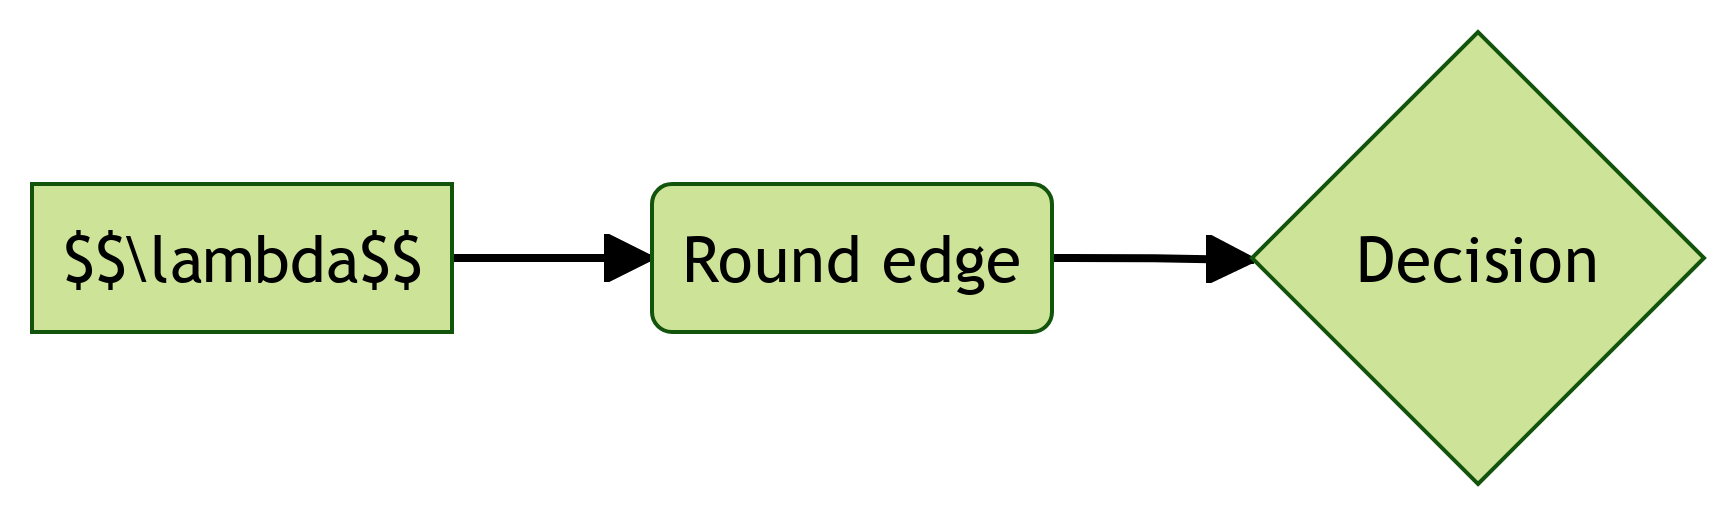
\includegraphics[width=5.5in,height=3.4in]{TCC_files/figure-latex/mermaid-figure-1.png}

}

\caption{\label{fig-arvore}Exemplo de estrutura de árvore de regressão.
A árvore tem cinco folhas e quatro nós internos.}

\end{figure}%

\vspace{12pt}

O espaço dos preditores é dividido em \(J\) regiões distintas e
disjuntas denotadas por \(R_1, R_2, \dots, R_J\). Essas regiões são
construídas em formato de caixa de forma a minimizar a soma dos
quadrados dos resíduos. Dessa forma, pode-se modelar a variável resposta
como uma constante \(c_j\) em cada região \(R_j\)

\[
f\left(x\right) = \sum^J_{j=1}c_j I\left(x \in R_j \right)
\]

O estimador para a constante \(c_j\) é encontrado pelo método de mínimos
quadrados. Assim, deve-se minimizar
\(\sum_{x_i \in R_j} \left[y_i - f\left(x_i\right)\right]^2\). No
entanto, perceba que \(f\left(x_i\right)\) está sendo avaliado somente
em um ponto específico \(x_i\), o que reduzirá \(f\left(x_i\right)\)
para uma constante \(c_j\). É fácil de se chegar ao resultado se for
observada a definição da função indicadora \(I\left(x \in R_j\right)\)

\[
I_{R_j}(x_i) =
\begin{cases}
    1,& \text{se } x_i \in R_j \\
    0,& \text{se } x_i \notin R_j
\end{cases}
\]

Como as regiões são disjuntas, \(x_i\) não pode estar simultaneamente em
duas regiões. Assim, para um ponto específico \(x_i\), apenas um dos
casos da função indicadora será diferente de 0. Portanto,
\(f\left(x_i\right) = c_j\). Agora, derivando
\(\sum_{x_i \in R_j}\left(yi - c_j\right)^2\) em relação a \(c_j\)

\begin{equation}\phantomsection\label{eq-partialdev}{
\frac{\partial}{\partial{c_j}}\sum_{x_i \in R_j} \left(y_i - c_j\right)^2 = -2\sum_{x_i \in R_j} \left(y_i - c_j\right)
}\end{equation} e igualando Equação~\ref{eq-partialdev} a 0, tem-se a
seguinte igualdade

\[
\sum_{x_i \in R_j} \left(y_i - \hat{c}_j\right) = 0
\] que se abrirmos o somatório e dividirmos pelo número total de pontos
\(N_j\) na região \(R_j\), teremos que o estimador de \(c_j\) será
simplesmente a média dos \(y_i\) na região \(R_j\):

\begin{equation}\phantomsection\label{eq-estimacjdev}{
\sum_{x_i \in R_j} y_i - \hat{c}_j N_j = 0 \Rightarrow \hat{c}_j = \frac{1}{N_{j}}\sum_{x_i \in R_j} y_i
}\end{equation}

\vspace{12pt}

No entanto, JAMES \emph{et al.} (2013) caracteriza como inviável
considerar todas as possíveis partições do espaço das variáveis em \(J\)
caixas devido ao alto custo computacional. Dessa forma, a abordagem a
ser adotada é uma divisão binária recursiva. O processo começa no topo
da árvore de regressão, o ponto em que contém todas as observações, e
continua sucessivamente dividindo o espaço dos preditores. As divisões
são indicadas como dois novos ramos na árvore, como pode ser visto na
Figura~\ref{fig-arvore}.

\vspace{12pt}

Para executar a divisão binária recursiva, deve-se primeiramente
selecionar a variável independente \(X_j\) e o ponto de corte \(s\) tal
que a divisão do espaço dos preditores conduza a maior redução possível
na soma dos quadrados dos resíduos. Dessa forma, definimos dois
semi-planos

\[
R_{1}\left(j, s\right) = \{X | X_j \leq s\} \text{ e } R_{2}\left(j, s\right) = \{X | X_j > s\}
\] e procuramos a divisão da variável \(j\) e o ponto de corte \(s\) que
resolve a equação

\[
\min_{j, s}\left[\min_{c_1} \sum_{x_i \in R_1\left(j, s\right)} \left(y_i - c_{1}\right)^2 + \min_{c_2} \sum_{x_i \in R_2\left(j, s\right)} \left(y_i - c_{2}\right)^2\right]
\] em que \(c_1\) e \(c_2\) é a média da variável dependente para as
observações de treinamento nas regiões \(R_1\left(j, s\right)\) e
\(R_2\left(j, s\right)\), respectivamente. Assim, encontrando a melhor
divisão, os dados são particionados nas duas regiões resultantes e o
processo de divisão é repetido em todas as outras regiões.

\vspace{12pt}

O tamanho da árvore pode ser considerado um hiperparâmetro para regular
a complexidade do modelo, pois uma árvore muito grande pode causar
sobreajuste aos dados de treinamento, capturando não apenas os padrões
relevantes, mas também o ruído. Como resultado, o modelo pode apresentar
bom desempenho nos dados de treinamento, mas falhar ao lidar com novos
dados devido à sua incapacidade de generalização. Por outro lado, uma
árvore muito pequena pode não captar padrões, relações e estruturas
importantes presentes nos dados. Dessa forma, a estratégia adotada para
selecionar o tamanho da árvore consiste em crescer uma grande árvore
\(T_0\), interrompendo o processo de divisão apenas ao atingir um
tamanho mínimo de nós. Posteriormente, a árvore \(T_0\) é podada
utilizando o critério de custo complexidade, que será definido a seguir.

\vspace{12pt}

Para o processo de poda da árvore, definimos uma árvore qualquer \(T\)
que pode ser obtida através do processo da poda de \(T_0\), de modo que
\(T \subset T_0\). Assim, sendo \(N_j\) a quantidade de pontos na região
\(R_j\), seja

\[
Q_j\left(T\right) = \frac{1}{N_j} \sum_{x_i \in R_j}\left(y_i - \hat{c}_j\right)^2
\] uma medida de impureza do nó pelo erro quadrático médio. Assim,
define-se o critério de custo complexidade

\[
C_{\alpha}\left(T\right) = \sum_{m = 1}^{|T|}N_jQ_j\left(T\right) + \alpha |T|
\] onde \(|T|\) denota a quantidade total de folhas, e \(\alpha \geq 0\)
é um hiperparâmetro que equilibra o tamanho da árvore e a adequação aos
dados. A ideia é encontrar, para cada \(\alpha\), a árvore
\(T_{\alpha} \subset T_0\) que minimiza \(C_{\alpha}\left(T\right)\).
Valores grandes de \(\alpha\) resultam em árvores menores, enquanto
valores menores resultam em árvores maiores, e \(\alpha = 0\) resulta na
própria árvore \(T_0\). A busca por \(T_{\alpha}\) envolve colapsar
sucessivamente o nó interno que provoca o menor aumento em
\(\sum_j N_j Q_j\left(T\right)\), continuando o processo até produzir
uma árvore com um único nó. Esse processo gera uma sequência de
subárvores, na qual existe uma única subárvore menor que, para cada
\(\alpha\), minimiza \(C_{\alpha}\left(T\right)\).

\vspace{12pt}

A estimação de \(\alpha\) é realizada por validação cruzada com cinco ou
dez folds, sendo \(\hat \alpha\) escolhido para minimizar a soma dos
quadrados dos resíduos durante o processo de validação cruzada. Assim, a
árvore final será \(T_{\hat \alpha}\). O
 Algoritmo~\ref{algo-buildtree}  exemplifica o processo de crescimento
de uma árvore de regressão:

\begin{algo}

\centering{

\begin{algorithm}[H]
\caption{Algoritmo para crescer uma árvore de regressão}
\begin{algorithmic}
\State \textbf{1.} Use a divisão binária recursiva para crescer uma árvore grande $T_0$ nos dados de treinamento, parando apenas quando cada folha tiver menos do que um número mínimo de observações.

\vspace{3.7pt}

\State \textbf{2.} Aplique o critério custo de complexidade à árvore grande \( T_0 \) para obter uma sequência de melhores subárvores \( T_\alpha \), em função de \( \alpha \).

\vspace{3.7pt}

\State \textbf{3.} Use validação cruzada $K\text{-fold}$ para escolher \( \alpha \). Isto é, divida as observações de treinamento em $K$ folds. Para cada \( k = 1, \ldots, K \):
    \State \hspace{1em} (a) Repita os Passos 1 e 2 em todos os folds, exceto no $k\text{-ésimo}$ fold dos dados de
    \State \hspace{1em} treinamento.
    \State \hspace{1em} (b) Avalie o erro quadrático médio de previsão nos dados no $k\text{-ésimo}$ fold deixado
    \State \hspace{1em} de fora, em função de \( \alpha \). Faça a média dos resultados para cada valor de \( \alpha \) e
    \State \hspace{1em} escolha \( \alpha \) que minimize o erro médio.

\vspace{3.7pt}

\State \textbf{4.} Retorne a subárvore \( T_{\hat{\alpha}} \) do Passo 2 que corresponde ao valor estimado de \( \alpha \).
\end{algorithmic}
\end{algorithm}

}

\caption{\label{algo-buildtree}Fonte: JAMES \emph{et al.} (2013, p.
337).}

\end{algo}%

\vspace{12pt}

No caso de uma árvore de decisão para classificação, a principal
diferença está no critério de divisão dos nós e na poda da árvore. Para
a classificação, a previsão em um nó \(j\), correspondente a uma região
\(R_j\) com \(N_j\) observações, será simplesmente a classe majoritária.
Assim, tem-se

\[
\hat{p}_{jk} = \frac{1}{N_j}\sum_{x_i \in R_j} I\left(y_i = k\right)
\] como a proporção de observações da classe \(k\) no nó \(j\). Dessa
forma, as observações no nó \(j\) são classificadas na classe
\(k\left(j\right) = \arg \max_{k} \hat{p}_{jk}\), que é a moda no nó
\(j\).

\vspace{12pt}

Para a divisão dos nós no caso da regressão, foi utilizado o erro
quadrático médio como medida de impureza. Para a classificação, algumas
medidas comuns para \(Q_j\left(T\right)\) são o erro de classificação, o
índice de Gini ou a entropia cruzada.

\section{Métodos Ensemble}\label{muxe9todos-ensemble}

~~~As árvores de decisão são conhecidas por sua alta interpretabilidade,
mas geralmente apresentam um desempenho preditivo inferior em comparação
com outros modelos e algoritmos. No entanto, é possível superar essa
limitação construindo um modelo preditivo que combina a força de uma
coleção de estimadores base, um processo conhecido como aprendizado em
conjunto (Ensemble Learning). De acordo com HASTIE \emph{et al.} (2009),
o aprendizado em conjunto pode ser dividido em duas etapas principais: a
primeira etapa consiste em desenvolver uma população de algoritmos de
aprendizado base a partir dos dados de treinamento, e a segunda etapa
envolve a combinação desses algoritmos para formar um estimador
agregado. Portanto, nesta seção, serão definidos os métodos de
aprendizado em conjunto utilizados neste trabalho.

\subsection{Bagging}\label{bagging}

~~~O algoritmo de Bootstrap Aggregation, ou Bagging, foi introduzido por
BREIMAN (1996). Sua ideia principal é gerar um estimador agregado a
partir de múltiplas versões de um preditor, que são criadas por meio de
amostras bootstrap do conjunto de treinamento, utilizadas como novos
conjuntos de treinamento. O Bagging pode ser empregado para melhorar a
estabilidade e a precisão de modelos ou algoritmos de aprendizado de
máquina, além de reduzir a variância e evitar o sobreajuste. Por
exemplo, o Bagging pode ser utilizado para melhorar o desempenho da
árvore de regressão descrita anteriormente.

\vspace{12pt}

BREIMAN (1996) define formalmente o algoritmo de Bagging, que utiliza um
conjunto de treinamento \(\mathcal{L}\). A partir desse conjunto, são
geradas amostras bootstrap \(\mathcal{L}^{(B)}\) com \(B\) réplicas,
formando uma coleção de modelos \(\{f(x, \mathcal{L}^{(B)})\}\), onde
\(f\) representa um modelo estatístico ou algoritmo treinado nas
amostras bootstrap para prever ou classificar uma variável dependente
\(y\) com base em variáveis independentes \(\mathbf{x}\). Se a variável
dependente \(y\) for numérica, a predição é obtida pela média das
previsões dos modelos:

\[
f_{B}\left(x\right) = \frac{1}{B} \sum_{b = 1}^B f \left(x, \mathcal{L}^{\left(B\right)}\right)
\] onde \(f_{B}\) representa a predição agregada. No caso em que \(y\)
prediz uma classe, utiliza-se a votação majoritária. Ou seja, se
estivermos classificando em classes \(j \in {1, \dots, J}\), então
\(N_j = \#\{B; f(x, \mathcal{L}^{(b)}) = j\}\) representa o número de
vezes que a classe \(j\) foi predita pelos estimadores. Assim,

\[
f_{B}\left(x\right) = \arg \max_{j} N_j
\] isto é, o \(j\) para o qual \(N_j\) é máximo

\vspace{12pt}

Embora a técnica de Bagging possa melhorar o desempenho de uma árvore de
regressão ou de classificação, isso geralmente vem ao custo de menor
interpretabilidade. Quando o Bagging é aplicado a uma árvore de
regressão, construímos \(B\) árvores de regressão usando \(B\) réplicas
de amostras bootstrap e tomamos a média das predições resultantes (JAMES
\emph{et al.}, 2013). Nesse processo, as árvores de regressão crescem
até seu máximo, sem passar pelo processo de poda, resultando em cada
árvore individual com alta variância e baixo viés. No entanto, ao
agregar as predições das \(B\) árvores, a variância é reduzida.

\vspace{12pt}

Para mitigar a falta de interpretabilidade do método Bagging aplicado a
árvores de regressão, pode-se usar a medida de impureza baseada no erro
quadrático médio, definida anteriormente, como uma métrica de
importância das variáveis independentes. Um valor elevado na redução
total média do erro quadrático médio, calculado com base nas divisões
realizadas por um determinado preditor em todas as \(B\) árvores, indica
que o preditor é importante.

\vspace{12pt}

As árvores construídas pelo algoritmo de árvore de decisão se beneficiam
da proposta de agregação do Bagging, mas esse benefício é limitado
devido à correlação positiva existente entre as árvores. Se as árvores
forem variáveis aleatórias independentes e identicamente distribuídas,
cada uma com variância \(\sigma^2\), a variância da média das previsões
das \(B\) árvores será \(\frac{1}{B} \sigma^2\). No entanto, se as
árvores forem apenas identicamente distribuídas, mas não necessariamente
independentes, e apresentarem uma correlação positiva \(\rho\), a
esperança da média das \(B\) árvores será a mesma que a esperança de uma
árvore individual. Portanto, o viés do agregado das árvores é o mesmo
das árvores individuais, e a melhoria é alcançada apenas pela redução da
variância. A variância da média das previsões será dada por:

\begin{equation}\phantomsection\label{eq-cor}{
\rho \sigma^2 + \frac{1 - \rho}{B}\sigma^2
}\end{equation}

Isso significa que, à medida que o número de árvores \(B\) aumenta, o
segundo termo da soma se torna menos significativo. Portanto, os
benefícios da agregação proporcionados pelo algoritmo de Bagging são
limitados pela correlação entre as árvores (HASTIE \emph{et al.}, 2009).
Mesmo com o aumento do número de árvores no Bagging, a correlação entre
elas impede que as previsões individuais sejam completamente
independentes, resultando em menor diminuição da variância da média das
previsões do que seria esperado se as árvores fossem totalmente
independentes. Uma maneira de melhorar o algoritmo de Bagging é por meio
do Random Forest, que será descrito a seguir.

\subsection{Random Forest}\label{random-forest}

\begin{algo}

\centering{

\begin{algorithm}[H]
\caption{Algoritmo de uma Random Forest para regressão ou classificação}
\begin{algorithmic}
\State \hspace{1em} \textbf{1.} Para b = 1 até B:

\vspace{0.8em}

    \State \hspace{2em} (a) Construa amostras bootstrap $\mathbf{\mathcal{L}}^*$ de tamanho \( N \) dos dados de
    \State \hspace{2em} \vspace{0.1em} treinamento.

    \State \hspace{2em} (b) Faça crescer uma árvore de floresta aleatória \( T_b \) para os dados bootstrap,
    \State \hspace{2em} repetindo recursivamente os seguintes passos para cada folha da árvore, até que
    \State \hspace{2em} \vspace{0.5em} o tamanho mínimo do nó \( n_{min} \) seja atingido.
    \State \hspace{4em} \vspace{0.1em} i. Selecione \( m \) variáveis aleatoriamente entre as \( p \) variáveis.
    \State \hspace{4em} \vspace{0.1em} ii. Escolha a melhor variável entre as \( m \).
    \State \hspace{4em} \vspace{0.1em} iii. Divida o nó em dois subnós.

\vspace{0.8em}

\State \hspace{1em} \textbf{2.} Por fim, o conjunto de árvores \( \{T_b\}^{B}_1\) é construído.

\vspace{1em}

\State \hspace{0.7em} No caso da regressão, para fazer uma predição em um novo ponto \( x \), temos a seguinte função:


$$
\hat{f}^{B}_{rf}\left(x\right) = \frac{1}{B}\sum^{B}_{b = 1} T_{b}\left(x\right)
$$

\vspace{1em}

\State \hspace{0.7em} Para a classificação é utilizado o voto majoritário. Assim, seja $\hat{C}_{b}\left(x\right)$ a previsão da classe da árvore de floresta aleatória $b$. Então,

$$
\hat{C}^{B}_{rf}\left(x\right) = \arg \max_c \sum^{B}_{b = 1}I\left(\hat{C}_b\left(x\right) = c\right)
$$

\State onde $c$ representa as classes possíveis.

\end{algorithmic}
\end{algorithm}

}

\caption{\label{algo-rf}Fonte: HASTIE \emph{et al.} (2009, p. 588).}

\end{algo}%

~~~O algoritmo Random Forest é uma técnica derivada do método de
Bagging, mas com modificações específicas na construção das árvores. O
objetivo é melhorar a redução da variância ao diminuir a correlação
entre as árvores, sem aumentar significativamente a variabilidade. Isso
é alcançado durante o processo de crescimento das árvores por meio da
seleção aleatória de variáveis independentes.

\vspace{12pt}

No algoritmo Random Forest, ao construir uma árvore a partir de amostras
bootstrap, selecionam-se aleatoriamente \(m \leq p\) das \(p\) variáveis
independentes como candidatas para a divisão, antes de cada ramificação
(com \(m = p\) no caso do Bagging). Dessa forma, diferente do Bagging,
aqui não se considera todas as \(p\) variáveis independentes para
realizar a divisão e minimizar a impureza, mas apenas \(m\) dessas \(p\)
variáveis. A escolha aleatória de apenas \(m\) covariáveis como
candidatas para a divisão ajuda a solucionar um dos principais problemas
do algoritmo de Bagging, que tende a gerar árvores de decisão
semelhantes, resultando em previsões altamente correlacionadas. O Random
Forest busca diminuir esse problema ao criar oportunidades para que
diferentes preditores sejam considerados. Em média, uma fração
\((p -m)/ p\) das divisões nem sequer incluirá o preditor mais forte
como candidato, permitindo que outros preditores tenham a chance de
serem selecionados (JAMES \emph{et al.}, 2013). Esse mecanismo reduz a
correlação entre as árvores, o que, por sua vez, diminui a variabilidade
das predições produzidas pelas árvores.

\vspace{12pt}

A quantidade de variáveis independentes \(m\) selecionadas
aleatoriamente é um hiperparâmetro que pode ser estimado por meio de
validação cruzada. Valores comuns para \(m\) são
\(m=\sqrt{p}\)\hspace{0pt} com tamanho mínimo do nó igual a um para
classificação, e \(m=p/3\)\hspace{0pt} com tamanho mínimo do nó igual a
cinco para regressão (HASTIE \emph{et al.}, 2009). Quando o número de
variáveis é grande, mas poucas são realmente relevantes, o algoritmo
Random Forest pode ter um desempenho inferior com valores pequenos de
\(m\), pois isso reduz as chances de selecionar as variáveis mais
importantes. No entanto, usar um valor pequeno de \(m\) pode ser
vantajoso quando há muitos preditores correlacionados. Além disso, assim
como no Bagging, a Random Forest não sofre de sobreajuste com o aumento
da quantidade de árvores \(B\). Portanto, é suficiente usar um \(B\)
grande o bastante para que a taxa de erro se estabilize (JAMES \emph{et
al.}, 2013).

\subsection{Boosting Trees}\label{boosting-trees}

~~~O Boosting, assim como o Bagging, é um método destinado a melhorar o
desempenho de modelos ou algoritmos. No entanto, neste trabalho, o
Boosting foi aplicado apenas às árvores de regressão. Portanto, a
explicação do Boosting será restrito ao caso de Boosting Trees
( Algoritmo~\ref{algo-boos} ).

\vspace{12pt}

\begin{algo}

\centering{

\begin{algorithm}[H]
\caption{Método Boosting aplicado a árvores de regressão}
\begin{algorithmic}
\State \hspace{1em} \textbf{1.} Defina $\hat{f}\left(x\right) = 0 \text{ e } r_i = y_i$ para todos os $i$ no conjunto de treinamento

\vspace{0.8em}

\State \hspace{1em} \vspace{0.8em} \textbf{2.} Para $b = 1, 2, \dots, B$, repita:

  \State \hspace{2em} (a) Ajuste uma árvore $\hat{f}^b$ com $d$ divisões para os dados de
  \State \hspace{2em} \vspace{0.1em} treinamento $\left(X, r\right)$.

  \State \hspace{2em} (b) Atualize $\hat{f}$ adicionando uma versão com o hiperparâmetro $\lambda$ de taxa de
  \State \hspace{2em} aprendizado:

$$
\hat{f}\left(x\right) \gets \hat{f}\left(x\right) + \lambda \hat{f}^b\left(x\right)
$$

  \vspace{0.1em}

  \State \hspace{2em} (c) Atualize os resíduos,

$$
r_i \gets r_i - \lambda \hat{f}^b\left(x_{i}\right)
$$

\vspace{1em}

\State \hspace{1em} \textbf{3.} Retorne o modelo de boosting,

$$
\hat{f}\left(x\right) = \sum_{b = 1}^B \lambda \hat{f}^b\left(x\right)
$$


\end{algorithmic}
\end{algorithm}

}

\caption{\label{algo-boos}Fonte: JAMES \emph{et al.} (2013, p. 349).}

\end{algo}%

No algoritmo de Bagging, cada árvore é construída e ajustada utilizando
amostras bootstrap, e ao final, um estimador agregado
\(\varphi_B\)\hspace{0pt} é formado a partir das \(B\) árvores. O
Boosting Trees funciona de maneira semelhante, mas sem o uso de amostras
bootstrap. A ideia principal é corrigir os erros das árvores anteriores,
ajustando as novas árvores aos resíduos das anteriores, visando melhorar
suas previsões. Assim, as árvores são construídas de forma sequencial,
incorporando as informações das árvores anteriores.

\vspace{12pt}

No caso da regressão, o Boosting combina um grande número de árvores de
decisão \(\hat{f}^1, \dots, \hat{f}^B\). A primeira árvore é construída
utilizando o conjunto de dados original, e seus resíduos são calculados.
Com a primeira árvore ajustada, a segunda árvore é ajustada aos da
árvore anterior resíduos e, em seguida, é adicionada ao estimador para
atualizar os resíduos. Dessa forma, os resíduos servem como informação
crucial para construir novas árvores e corrigir os erros das árvores
anteriores. Como cada nova árvore depende das árvores já construídas,
árvores menores são suficientes (JAMES \emph{et al.}, 2013).

\vspace{12pt}

O processo de aprendizado no método de Boosting é lenta, o que acaba
gerando melhores resultados. Esse processo de aprendizado pode ser
controlado por um hiperparâmetro \(\lambda\) chamado de shrinkage, ou
taxa de aprendizado, permitindo que mais árvores, com formas diferentes,
corrijam os erros das árvores passadas. No entanto, um valor muito
pequeno para \(\lambda\) requer uma quantidade muito maior \(B\) de
árvores e, diferente do Bagging e Random Forest, o Boosting pode sofrer
de sobreajuste se a quantidade de árvores é muito grande. Além disso, a
quantidade de divisões \(d\) em cada árvore, que controla a complexidade
do boosting, pode ser considerado também um hiperparâmetro. Para
\(d = 1\) é ajustado um modelo aditivo, já que cada termo involve apenas
uma variável. JAMES \emph{et al.} (2013) define \(d\) como a
profundidade de interação que controla a ondem de interação do modelo
boosting, já que \(d\) divisões podem envolver no máximo \(d\)
variáveis.

\subsection{Stacked generalization}\label{stacked-generalization}

~~~A Stacked Generalization, ou Stacking, é um método de ensemble que
consiste em treinar um modelo gerado a partir da combinação da predição
de vários outros modelos, visando melhorar a precisão das predições.
Esse método pode ser aplicado a qualquer modelo estatístico ou algoritmo
de aprendizado de máquina. A ideia principal é atribuir pesos às
predições, de modo a dar maior importância aos modelos que produzem
melhores resultados, ao mesmo tempo em que se evita atribuir altos pesos
a modelos com alta complexidade.

\vspace{12pt}

Matematicamente, o Stacking define predições
\(\hat{f}_m^{-i}\left(x\right)\) em x, utilizando o modelo \(m\),
aplicado ao conjunto de treinamento com a \(i\text{-ésima}\) observação
removida (HASTIE \emph{et al.}, 2009). Assim, os peso são estimados de
forma a minimizar o erro de predição combinado, dado pela seguinte
expressão:

\[
\hat{w}^{st} = \arg \min_{w} \sum^{N}_{i = 1} \left[y_i - \sum^{M}_{m = 1} w_m f^{-i}_m\left(x_i\right)\right]^2
\] A previsão final dos modelos empilhados é
\(\sum_{m} \hat{w}_m^{st} \hat{f}_m\left(x\right)\). Assim, em vez de
escolher um único modelo, o método de Stacking combina os modelos
utilizando pesos estimados, o que melhora a performance preditiva, mas
pode comprometer a interpretabilidade.

\subsection{Gradient Boosting}\label{gradient-boosting}

~~~O algoritmo de Gradient Boosting é semelhante ao de Boosting, mas com
diferenças mínimas. Ele constrói modelos aditivos ajustando
sequencialmente funções bases aos pseudos-resíduos, que correspondem aos
gradientes da função perda do modelo atual (FRIEDMAN, 2002). Esses
gradientes indicam a direção na qual a função perda diminui. Neste
trabalho, foram utilizadas diferentes implementações de Gradient
Boosting. No entanto, todas empregam o Gradient Boosting com árvores de
regressão, com algumas modificações para a construção das árvores ou
para melhorar a eficiência do algoritmo existente. Assim, o algoritmo a
ser explicado será o Gradient Tree Boosting
( Algoritmo~\ref{algo-gradboos} ).

\begin{algo}

\centering{

\begin{algorithm}[H]
\caption{Gradient Tree Boosting}
\begin{algorithmic}
\State \hspace{1em} \textbf{1.} Inicialize $f_0\left(x\right) = \arg \min_{\gamma} \sum_{i = 1}^N L\left(y_i, \gamma \right)$

\vspace{0.8em}

\State \hspace{1em} \vspace{0.8em} \textbf{2.} Para $m = 1$ até $M$:

  \State \hspace{2em} (a) Para $i = 1, 2, \dots, N$, calcule

$$
{r}_{im} = -\left[\frac{\partial L\left(y_i, f\left(x_i \right)\right)}{\partial f\left(x_i\right)}\right]_{f = f_{m - 1}}
$$

  \State \hspace{2em} (b) Ajuste uma árvore de regressão aos pseudo-resíduos $r_{im}$, obtendo regiões
  \State \hspace{2em} terminais $R_{jm}, \ j = 1, 2, \dots, J$.


  \State \vspace{0.1em}

  \State \hspace{2em} (c) Para $j = 1, 2, \dots, J_m$, calcule

$$
\gamma_{jm} = \arg \min_{\gamma} \sum_{x_i \in R_{jm}} L\left(y_i, f_{m - 1}\left(x_i\right) + \gamma\right)
$$

  \vspace{0.1em}

  \State \hspace{2em} (d) Atualize $f_m\left(x\right) = f_{m - 1}\left(x\right) + \lambda \sum^{J}_{j = 1} \gamma_{jm} I\left(x \in R_{jm}\right)$

\vspace{1em}

\State \hspace{1em} \textbf{3.} Retorne $\hat{f}\left(x\right) = f_M\left(x\right)$

\end{algorithmic}
\end{algorithm}

}

\caption{\label{algo-gradboos}Fonte: HASTIE \emph{et al.} (2009, p.
361).}

\end{algo}%

\vspace{12pt}

O Gradient Boosting aplicado para árvores de regressão, tem que cada
função base é uma árvore de regressão com \(J_m\) folhas. Dessa forma,
cada árvore de regressão tem a forma aditiva

\begin{equation}\phantomsection\label{eq-treebost}{
h_m\left(x;\{b_j, R_j\}^J_{1}\right) = \sum^{J_m}_{j = 1} b_{jm} I\left(x \in R_{jm}\right)
}\end{equation} em que \(\{R_{jm}\}^{J_m}_{1}\) são as regiões disjuntas
que, coletivamente, cobrem o espaço de todos os valores conjuntos das
variáveis preditoras \(\mathbf{x}\). Essas regiões são representadas
pelas folhas de sua correspondente árvore. Como as regiões são
disjuntas, Equação~\ref{eq-treebost} se reduz simplesmente a
\(h_m\left(x\right) = b_{jm}\text{ para } x \in  R_{jm}\). Por mínimos
quadrados, \(b_{jm}\) é simplesmente a média dos pseudo-resíduos
\(r_{im}\),

\[
\hat{b}_{jm} = \frac{1}{N_{jm}} \sum_{x_i \in R_{jm}} r_{im}
\] que dão a direção de diminuição da função perda \(L\) pela expressão
do gradiente da linha 2(a). Assim, cada árvore de regressão é ajustada
aos \(r_{im}\) de forma a minimizar o erro das árvores anteriores.
\(N_{jm}\) denota a quantidade de pontos na região \(R_{jm}\). Por fim,
o estimador é separadamente atualizado em cada região correspondente e é
expresso

\[
f_m\left(x\right) = f_{m - 1}\left(x\right) + \lambda \sum^{J}_{j = 1} \gamma_{jm} I\left(x \in R_{jm}\right)
\] em que \(\gamma_{jm}\) representa a atualização da constante ótima
para cada região, baseado na função perda \(L\), dada a aproximação
\(f_{m-1}\left(x\right)\). O \(0 < \lambda \leq 1\), assim como no
algoritmo de boosting, representa o hiperparâmetro shrinkage para
controlar a taxa de aprendizado. Pequenos valores de \(\lambda\)
necessitam maiores quantidades de iterações \(M\) para diminuir o risco
de treinamento.

\vspace{12pt}

As outras implementações de Gradient Boosting aplicadas à árvores de
decisão tem seus próprios motivos de existência. Esses motivos incluem a
busca por maior eficiência computacional, adição de recursos e até mesmo
maior flexibilidade. As duas outras implementações utilizadas foram o
Extreme Gradient Boosting e Light Gradient Boosting.

\vspace{12pt}

O Extreme Gradient Boosting (CHEN; GUESTRIN, 2016) é uma implementação
altamente eficiente do algoritmo e flexível de Gradient Boosting
aplicado à árvores de decisão. Além disso, é adicionado um novo recurso,
técnicas de regularização para diminuir o sobreajuste do modelo. A
função objetivo agora passa a ser definida da seguinte forma:

\[
\mathcal{L}\left(\phi\right) = \sum_{i}l\left(\hat{y}_{i}, y_{i}\right) + \sum_{k}\Omega\left(f_{k}\right)
\] em que \(l\) é uma função de perda convexa diferenciável e o segundo
termo \(Omega\) penaliza a complexidade de cada função de árvore de
decisão. O termo de regularização adicional ajuda a suavizar os pesos
finais para evitar o sobreajuste. \(\Omega\) é definido dado como:

\[
\Omega\left(f\right) = \gamma T + \frac{1}{2}\lambda\|\omega\|^{2}
\] onde \(T\) é a quantidade de folhas na árvore, \(\|\omega\|^{2}\) é a
soma do quadrado dos pesos associados às folhas. \(\gamma\) e
\(\lambda\) são os parâmetros de regularização, em que \(\lambda\)
penaliza os pesos das folhas e \(\gamma\) penaliza a quantidade de
folhas nas árvores. Além disso, é fácil ver que
\(\frac{1}{2}\lambda\|\omega\|^{2}\) representa a penalização L2
(Ridge). Assim, com a regularização aplicada a função objetivo, modelos
e funções preditivas serão mais comuns pois simplificarão o modelo. As
implementações do algoritmo de Extreme Gradient Boosting presentes em
Python utilizam a regularização L2 como padrão, mas também permitem o
uso da regularização L1 (Lasso).

\vspace{12pt}

Assim como o Gradient Boosting, as implementações existentes de Light
Gradient Boosting também permite utilizar a regularização L1 ou L2, mas
não utiliza nenhuma das duas por padrão. A principal diferença do Light
Gradient Boosting está na forma de crescimento das árvores, primeiro é
dividido a folha com a maior redução na função de erro. Além disso, tem
um grande foco na velocidade e uma melhor eficiência no uso da memória
atráves do algoritmo de Histogram-Based. Esse algoritmo faz com que
invés de avaliar cada ponto quando realiza a divisão, ele divide valores
contínuos em intervalos, como um histograma, o que reduz grandemente o
custo computacional.

\vspace{12pt}

\chapter{Metodologia}\label{metodologia}

\section{Obtenção dos dados}\label{obtenuxe7uxe3o-dos-dados}

~~~Os dados foram obtidos por meio de web scraping, uma técnica
automatizada de extração de informações de páginas web. Para isso, foram
utilizadas as linguagens de programação R e Python. No R, os pacotes
xml2 (WICKHAM; HESTER; OOMS, 2023) e rvest (WICKHAM, 2024) foram
utilizados para extrair dados de páginas estáticas de forma estruturada.
No Python, as bibliotecas Scrapy (KOUZIS-LOUKAS, 2016) e Playwright,
desenvolvida pela Microsoft, foram empregadas, sendo esta última
essencial para a interação com páginas dinâmicas, possibilitando a
extração de informações que exigem interações como cliques ou rolagem de
página. Além dessas ferramentas, foram implementadas técnicas de
rotacionamento de IPs e de modificação das informações do usuário que
acessa o site, a fim de evitar bloqueios durante o processo de coleta de
dados, garantindo assim a continuidade e eficácia da extração. A
ferramenta utilizada para a rotação das informações do usuário que
acessa o site é a API criada pela empresa ScrapeOps.

\vspace{12pt}

Assim, utilizando as ferramentas e técnicas de web scraping, foram
coletadas as variáveis que faziam sentido para a modelagem, priorizando
aquelas com menor probabilidade de gerar problemas durante o tratamento
dos dados. Ao todo, foram extraídas 25 variáveis, das quais 10 são
quantitativas e 15 qualitativas nominais, sendo 13 de caráter
dicotômico. No entanto, nem todas as variáveis foram obtidas diretamente
por web scraping. As coordenadas de latitude e longitude, por exemplo,
foram geradas por meio da geocodificação dos endereços, utilizando o
pacote tidygeocoder (CAMBON \emph{et al.}, 2021) da linguagem R. Dessa
forma, tem-se as seguintes variáveis:

\begin{itemize}
\item
  Valor do imóvel: variável dependente que será modelada e constitui o
  principal foco de análise deste trabalho;
\item
  Valor médio do aluguel no bairro: valor médio do aluguel dos imóveis
  no bairro, em \(m^3\);
\item
  Área: área total do imóvel, medida em \(m^2\);
\item
  Área média do aluguel no bairro: área média dos imóveis alugados no
  bairro, em \(m^2\);
\item
  Condomínio: valor mensal pago pelo condomínio do imóvel;
\item
  IPTU: imposto cobrado sobre imóveis urbanos;
\item
  Banheiros: quantidade de banheiros disponíveis na propriedade;
\item
  Vagas de estacionamento: número total de vagas de estacionamento
  disponíveis;
\item
  Quartos: quantidade de quartos no imóvel;
\item
  Latitude: posição horizontal, medida em frações decimais de graus;
\item
  Longitude: posição vertical, também medida em frações decimais de
  graus, assim como a latitude;
\item
  Tipo do imóvel: sete categorias foram consideradas: apartamentos,
  casas, casas comerciais, casas de condomínio, casas de vila,
  coberturas, e lotes comerciais e de condomínio;
\item
  Endereço: nome do endereço onde o imóvel está localizado;
\item
  Variáveis dicotômicas: indicam a presença (1) ou ausência (0) de
  determinadas características no imóvel, como área de serviço,
  academia, elevador, espaço gourmet, piscina, playground, portaria 24
  horas, quadra de esportes, salão de festas, sauna, spa e varanda
  gourmet.
\end{itemize}

\vspace{12pt}

No entanto, com base nas observações realizadas durante o estudo, nem
todas as variáveis coletadas foram utilizadas na modelagem do valor dos
imóveis. Algumas foram excluídas devido a uma quantidade excessiva de
valores ausentes, enquanto outras se mostraram pouco significativas para
explicar o valor do imóvel. Após o processo de coleta e limpeza dos
dados, o banco de dados final conta com 31.782 observações.

\section{Análise exploratória de
dados}\label{anuxe1lise-exploratuxf3ria-de-dados}

~~~A análise exploratória de dados é uma das primeiras etapas de
qualquer estudo que utiliza a estatística como ferramenta principal,
pois permite identificar padrões de comportamento nos dados e descobrir
relações entre as variáveis estudadas. Assim, após a coleta e
organização dos dados, a primeira etapa deste estudo consistiu em uma
análise descritiva. Essa análise possibilitou identificar padrões entre
os diferentes tipos de imóveis e como essas características podem
influenciar o seu valor. Para evidenciar esses comportamentos, foram
criados gráficos e tabelas que permitiram caracterizar as relações entre
as variáveis independentes e a variável dependente.

\section{Construção do modelo}\label{construuxe7uxe3o-do-modelo}

~~~No conjunto de dados extraído, foram avaliados diferentes modelos
para a previsão do valor do imóvel. Inicialmente, o valor do imóvel foi
explicado por variáveis consideradas relevantes para o estudo, como:
valor médio do aluguel no bairro, área, área média do aluguel no bairro,
número de banheiros, vagas de estacionamento, número de quartos,
latitude, longitude, tipo de imóvel e variáveis dicotômicas obtidas
durante o processo de extração. As variáveis relacionadas ao valor do
condomínio e IPTU foram excluídas do modelo devido à alta quantidade de
valores ausentes.

\vspace{12pt}

Com as variáveis selecionadas, o conjunto de dados foi dividido em
treino e teste para avaliar o desempenho dos modelos. A divisão foi
realizada de forma estratificada, utilizando a classe
StratifiedShuffleSplit, que garante uma amostragem estratificada e
aleatória. A estratificação foi baseada na variável ``tipo de imóvel'',
preservando a proporção de amostras para cada categoria. Definiu-se 20\%
do conjunto de dados para o teste, enquanto os 80\% restantes foram
reservados para o treinamento.

\vspace{12pt}

Para a aplicação das ferramentas de modelagem, foram utilizadas as
bibliotecas \texttt{scikit-learn}, \texttt{lightgbm} e \texttt{xgboost}.
As duas últimas foram empregadas especificamente na modelagem, enquanto
a primeira também foi utilizada para criar pipelines de
pré-processamento de dados, que organizam etapas sequenciais de
preparação necessárias para o tratamento adequado dos dados. Assim, os
quatro modelos aplicados na previsão do valor do imóvel foram: Random
Forest, Gradient Boosting, LightGBM e XGBoost. Por fim, foi implementado
o algoritmo de Stacking, combinando os modelos previamente construídos
para melhorar a performance preditiva. No Stacking, foi utilizado como
preditor final o algoritmo de Light Gradient Boosting.

\subsection{Etapas de
pré-processamento}\label{etapas-de-pruxe9-processamento}

~~~Após toda a organização e limpeza dos dados, foram aplicadas algumas
transformações com o objetivo de estabelecer uma relação compreensível
das variáveis que mais interferem no valor do imóvel. Além disso, foi
aplicado também o tratamento de valores ausentes presentes no conjunto
de dados.

\vspace{12pt}

O método utilizado para a imputação de valores ausentes foi o algoritmo
k-nearest neighbors (KNN). Esse algoritmo estima os valores ausentes de
acordo com a fórmula:

\[
\hat{y} = \frac{1}{k}\sum_{x_i \in N_k\left(x\right)}y_i
\] onde \(N_k(x)\) representa o conjunto de \(k\) vizinhos mais próximos
de \(x\), ou seja, os pontos \(x_i\) no conjunto de dados que estão mais
próximos de \(x\). Essa proximidade é geralmente medida pela distância
Euclidiana, que é a métrica padrão utilizada pela classe
\texttt{KNNImputer} da biblioteca scikit-learn para imputação de valores
ausentes. No processo de imputação, foi utilizado um total de 17
vizinhos, definido pelo argumento \texttt{n\_neighbors} da classe
\texttt{KNNImputer}.

\vspace{12pt}

A transformação utilizada para estabilizar a variância e aproximar a
distribuição dos regressores de uma distribuição normal foi a
transformação logarítmica. Para lidar com variáveis categóricas, foi
utilizada a classe OneHotEncoder, que aplica a codificação one hot. Essa
técnica transforma as categorias das variáveis em variáveis dicotômicas,
criando uma nova coluna para cada categoria. Além disso, o
OrdinalEncoder foi utilizado para variáveis ordinais, que possuem uma
ordem. Dessa forma, o OneHotEncoder foi aplicado à variável de tipo de
imóvel, transformando cada categoria de imóvel em variáveis dummy. Já o
OrdinalEncoder foi aplicado à variável de tamanho do imóvel, que foi
criada posteriormente para classificar os imóveis em diferentes faixas:
pequenos, médios e grandes.

\vspace{12pt}

Por fim, as variáveis numéricas foram normalizadas utilizando a classe
StandardScaler, que padroniza os dados aplicando a seguinte
transformação:

\[
z = \frac{x - \mu}{\sigma}
\] onde \(\mu\) é a média da amostra de treinamento e \(\sigma\) é o
desvio padrão da amostra de treinamento.

\subsection{Validação cruzada}\label{validauxe7uxe3o-cruzada}

~~~A técnica utilizada para validar o modelo, além das métricas, foi a
validação cruzada. A validação cruzada serve para estimar um erro de
generalização médio da seguinte forma
\(Err = E\left[L\left(Y, \hat{f}\left(X\right)\right)\right]\), em que
\(L\) é uma função perda e \(\hat f\) é um estimador. Existem diversar
técnicas de validação cruzada, a que foi utilizada nesse trabalho é a
validação cruzada K-Fold.

\vspace{12pt}

A validação cruzada K-Fold é uma técnica que utiliza parte dos dados
para ajustar o modelo e outra parte para testá-lo. Nessa abordagem, os
dados são divididos em \(K\) folds. Em cada iteração, um desses folds é
reservado para testar o modelo, enquanto os \(K−1\) folds restantes são
usados para treiná-lo. O modelo é ajustado nos \(K−1\) subconjuntos e
avaliado no subconjunto de teste, permitindo estimar o erro de predição.
Esse processo é repetido \(K\) vezes, alternando o subconjunto de teste
em cada rodada, e ao final, os \(K\) erros de predição são combinados. O
erro de predição estimado pela validação cruzada é dado por:

\[
CV\left(\hat f\right) = \frac{1}{N}\sum_{i = 1}^N L\left(y_i, \hat{f}^{-k\left(i\right)}\left(x_i\right)\right)
\] onde \(N\) é o número total de observações, \(L\) é a função de
perda, \(y_i\)\hspace{0pt} é o valor observado, \(x_i\)\hspace{0pt} é a
entrada correspondente, e \(\hat{f}^{-k\left(i\right)}\) é o modelo
ajustado sem o i-ésimo subconjunto.

\begin{figure}

\centering{

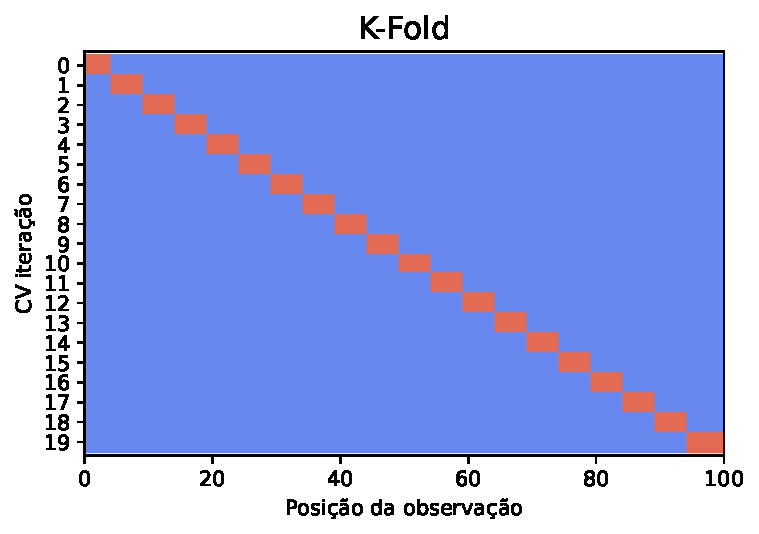
\includegraphics{TCC_files/figure-pdf/fig-kfold-output-1.pdf}

}

\caption{\label{fig-kfold}Visualização de K-Fold com 20 folds.}

\end{figure}%

\vspace{12pt}

A figura acima ilustra exatamente o caso da validação cruzada por
K-Fold. As divisões do conjunto de dados para treinamento do modelo são
representados pela cor azul, enquanto as laranjas são os conjuntos de
validação, onde o modelo ajustado será testado e validado com uma função
perda \(L\).

\vspace{12pt}

Para aplicar a validação cruzada com K-Fold nos modelos utilizados neste
trabalho, foi empregada uma função e uma classe da biblioteca
scikit-learn, ambas disponíveis no módulo model\_selection. A função
utilizada para a validação cruzada é a \texttt{cross\_val\_score}, na
qual o modelo a ser validado é passado por meio do argumento estimator.
O critério de avaliação é especificado no argumento \texttt{scoring}, e
a técnica de validação cruzada é definida pelo argumento cv. No caso
deste trabalho, foi utilizada a classe \texttt{KFold(n\_splits=20)},
responsável por realizar a validação cruzada com K-Fold. O argumento
\texttt{n\_splits} define o número de folds utilizados durante a
validação, que neste caso foram 20. Por fim, basta calcular a média das
métricas retornadas pelo \texttt{cross\_val\_score} para cada um dos
folds.

\vspace{12pt}

A métrica utilizada para avaliar o desempenho dos modelos durante a
validação cruzada foi a raiz do erro quadrático médio (RMSE). O RMSE
mede o quanto os valores estimados pelo modelo se afastam, em média, dos
valores observados, sendo que quanto menor o RMSE, melhor é o desempenho
do modelo. Além do RMSE, foi também utilizada a métrica MAPE (Erro
Percentual Absoluto Médio), que quantifica, em termos percentuais, o
desvio médio entre os valores estimados e os observados. Por fim, foi
analisado o coeficiente de determinação (\(R^2\)), uma medida que indica
a proporção da variação da variável dependente explicada pelas variáveis
independentes; neste caso, o valor do imóvel. As métricas são definidas
da seguinte forma:

\begin{figure}

\begin{minipage}{0.33\linewidth}
\[
\text{RMSE} = \sqrt{\dfrac{1}{n} \sum_{i = 0}^n (y_i - \hat y_i)^2}
\]\end{minipage}%
%
\begin{minipage}{0.33\linewidth}
\[
R^2 = 1 - \dfrac{SS_{\text{resíduos}}}{SS_{\text{total}}}
\]\end{minipage}%
%
\begin{minipage}{0.33\linewidth}
\[
\text{MAPE} = \frac{1}{n} \sum_{i=0}^n \left|1 - \frac{y_i}{\hat y_i}\right|
\]\end{minipage}%

\end{figure}%

\hfill\break
em que \(SS_{\text{resíduos}}\) e \(SS_{\text{total}}\) representam,
respectivamente, a soma dos quadrados dos resíduos e a soma dos
quadrados totais.

\section{Otimização de
hiperparâmetros}\label{otimizauxe7uxe3o-de-hiperparuxe2metros}

~~~Existem diversas técnicas para otimização de hiperparâmetros em
aprendizado de máquina. Uma das mais comuns é o GridSearch. Segundo
BISCHL \emph{et al.} (2023), o GridSearch consiste em dividir o
intervalo contínuo de valores possíveis de cada hiperparâmetro em um
conjunto de valores discretos, avaliando exaustivamente o algoritmo para
todas as combinações possíveis. No entanto, como o número de combinações
cresce exponencialmente com o aumento das combinações de
hiperparâmetros, o GridSearch apresenta um custo computacional elevado.
Por isso, existem métodos de otimização mais sofisticados que oferecem
melhor desempenho, como a otimização bayesiana, que foi utilizada neste
trabalho.

\vspace{12pt}

A otimização bayesiana não se refere a um algoritmo específico, mas sim
a uma abordagem de otimização fundamentada na inferência bayesiana, que
engloba uma ampla família de algoritmos (GARNETT, 2023). Além disso, a
otimização bayesiana tem alcançado benchmarks superiores em comparação
com outros algoritmos em diversos problemas complexos de otimização de
hiperparâmetros (SNOEK; LAROCHELLE; ADAMS, 2012).

\vspace{12pt}

Diferentemente de outros algoritmos de otimização de hiperparâmetros, a
otimização bayesiana ajusta suas tentativas futuras de avaliação com
base nos resultados obtidos anteriormente (YANG; SHAMI, 2020). Para
definir os pontos futuros, utiliza-se uma função probabilística
\(P\left(\rho |  \lambda \right)\) (BERGSTRA; YAMINS; COX, 2013). Após
ajustar essa função, obtém-se, para cada \(\lambda\), uma estimativa da
performance \(\hat c \left(\lambda \right)\) e da incerteza da predição
\(\hat \sigma \left(\lambda \right)\), além da distribuição preditiva
associada à função probabilística. Com essa distribuição, uma função de
aquisição determina o equilíbrio entre exploitation e
exploration\footnote{Exploitation refere-se à busca por soluções
  próximas a boas observações anteriores, enquanto exploration visa
  explorar áreas ainda não investigadas}. Assim, os algoritmos de
otimização bayesiana são regidos pela relação
\(\lambda \to c\left(\lambda \right)\) e buscam um equilíbrio entre
exploitation e exploration para identificar as regiões mais promissoras,
sem negligenciar possíveis configurações melhores em áreas ainda
inexploradas.

\subsection{Tree-Structured Parzen
Estimator}\label{tree-structured-parzen-estimator}

~~~A função probabilística utilizada para a otimização bayesiana neste
trabalho foi a Tree-Structured Parzen Estimator (TPE). O TPE define duas
funções, \(l\left(x\right)\) e \(g\left(x\right)\), que são utilizadas
para modelar a distribuição das variáveis do domínio (YANG; SHAMI,
2020). Essas duas densidades são empregadas para estimar a probabilidade
de se observar um hiperparâmetro \(x\), dado uma métrica de performance
\(\rho\). Assim, tem-se a seguinte definição:

\begin{equation}\phantomsection\label{eq-tpe}{
p(x|y) =
\begin{cases}
    l(x) & \text{if } y < y^* \\
    g(x) & \text{if } y \ge y^*
\end{cases}
}\end{equation} em que \(l\left(x\right)\) representa a densidade quando
a função de perda é menor que um limiar \(y^*\), e \(g\left(x\right)\) é
a densidade quando a função de perda tem valores acima de \(y^*\)
(BERGSTRA \emph{et al.}, 2011). O limite \(y^*\) é definido por um
hiperparâmetro \(\gamma\), onde \(\gamma\) corresponde ao percentil dos
valores observados de \(y\), de modo que
\(p\left(y < y^*\right) = \gamma\).

\vspace{12pt}

Por padrão, o Tree-Structured Parzen Estimator (TPE) utiliza como função
de aquisição o Expected Improvement (EI), que pode ser otimizado no TPE
da seguinte forma:

\begin{equation}\phantomsection\label{eq-exp}{
  EI_{y^*}\left(x\right) = \int_{-\infty}^{y^*} \left(y^* - y\right)p\left(y | x\right) dy
}\end{equation}

Para encontrar a probabilidade marginal de \(x\), temos a seguinte
integral:
\(p\left(x\right) = \int_{\mathbb{R}} p\left(x | y\right)p\left(y\right)dy\).
Particionando o domínio de \(y\), obtemos:

\[
p\left(x\right) = \gamma l\left(x\right) + \left(1 - \gamma \right) g\left(x\right)
\]

Assim, aplicando o Teorema de Bayes e substituindo na integral da
equação Equação~\ref{eq-exp}:

\[
EI_{y^*}\left(x\right) = \int_{-\infty}^{y^*} \left(y^* - y\right) \frac{p\left(x | y\right)p\left(y\right)}{p\left(x\right)}dy = \left(\gamma y^*  - \int_{-\infty}^{y^*} p\left(y\right)dy\right) \left(\gamma + \left(1 - \gamma\right)\frac{g\left(x\right)}{l\left(x\right)}\right) ^{-1}
\]

A segunda expressão do produto mostra que, para maximizar o Expected
Improvement, é necessário encontrar pontos de \(x\) com maior
probabilidade em \(l\left(x\right)\) e menor probabilidade em
\(g\left(x\right)\). No entanto, no TPE, maximizar o \(EI\) é
equivalente a maximizar a razão entre as duas distribuições, definida
como \(r\left(x\right) = \frac{l\left(x\right)}{g\left(x\right)}\)
(COWEN-RIVERS \emph{et al.}, 2022).

\vspace{12pt}

\subsection{Otimização de hiperparâmetros com
optuna}\label{otimizauxe7uxe3o-de-hiperparuxe2metros-com-optuna}

~~~Para otimizar os hiperparâmetros dos modelos foi utilizado a
bilbioteca \texttt{optuna} (AKIBA \emph{et al.}, 2019) da linguagem de
programação Python. Essa biblioteca implementa diversos métodos para
otimização automatizada de hiperparâmetros. Para a sua utilização, é
preciso definir inicialmente uma função objetivo. Por exemplo, para
otimizar os hiperparâmetros de uma random forest, seria necessário
definir uma função objetivo da seguinte forma:

\begin{Shaded}
\begin{Highlighting}[]
\ImportTok{import}\NormalTok{ optuna}
\ImportTok{import}\NormalTok{ numpy }\ImportTok{as}\NormalTok{ np}
\ImportTok{import}\NormalTok{ pandas }\ImportTok{as}\NormalTok{ pd}
\ImportTok{from}\NormalTok{ sklearn }\ImportTok{import}\NormalTok{ ensemble}
\ImportTok{from}\NormalTok{ sklearn.model\_selection }\ImportTok{import}\NormalTok{ cross\_val\_score, KFold}

\KeywordTok{def}\NormalTok{ objective(trial):}
\NormalTok{    X }\OperatorTok{=}\NormalTok{ train\_df[variaveis\_independentes]}
\NormalTok{    y }\OperatorTok{=}\NormalTok{ train\_df.variavel\_dependente}

\NormalTok{    params }\OperatorTok{=} \BuiltInTok{dict}\NormalTok{(}
\NormalTok{        n\_estimators}\OperatorTok{=}\NormalTok{trial.suggest\_int(}
\NormalTok{          name}\OperatorTok{=}\StringTok{\textquotesingle{}n\_estimators\textquotesingle{}}\NormalTok{,}
\NormalTok{          low}\OperatorTok{=}\DecValTok{1}\NormalTok{,}
\NormalTok{          high}\OperatorTok{=}\DecValTok{1000}\NormalTok{),}
\NormalTok{        max\_depth}\OperatorTok{=}\NormalTok{trial.suggest\_int(}
\NormalTok{          name}\OperatorTok{=}\StringTok{\textquotesingle{}max\_depth\textquotesingle{}}\NormalTok{,}
\NormalTok{          low}\OperatorTok{=}\DecValTok{20}\NormalTok{,}
\NormalTok{          high}\OperatorTok{=}\DecValTok{1000}\NormalTok{),}
\NormalTok{        max\_features}\OperatorTok{=}\StringTok{\textquotesingle{}sqrt\textquotesingle{}}\NormalTok{,}
\NormalTok{        random\_state}\OperatorTok{=}\DecValTok{42}
\NormalTok{    )}

\NormalTok{    model }\OperatorTok{=}\NormalTok{ ensemble.RandomForestRegressor(}
        \OperatorTok{*}\NormalTok{params}
\NormalTok{    )}
\NormalTok{    model.fit(X}\OperatorTok{=}\NormalTok{X, y}\OperatorTok{=}\NormalTok{y)}

\NormalTok{    cv\_scores }\OperatorTok{=}\NormalTok{ np.expm1(np.sqrt(}\OperatorTok{{-}}\NormalTok{cross\_val\_score(}
\NormalTok{        estimator}\OperatorTok{=}\NormalTok{model,}
\NormalTok{        X}\OperatorTok{=}\NormalTok{X,}
\NormalTok{        y}\OperatorTok{=}\NormalTok{y,}
\NormalTok{        scoring}\OperatorTok{=}\StringTok{"neg\_mean\_squared\_error"}\NormalTok{,}
\NormalTok{        n\_jobs}\OperatorTok{=}\DecValTok{3}\NormalTok{,}
\NormalTok{        cv}\OperatorTok{=}\NormalTok{KFold(n\_splits}\OperatorTok{=}\DecValTok{20}\NormalTok{))))}

    \ControlFlowTok{return}\NormalTok{ np.mean(cv\_scores)}

\NormalTok{study }\OperatorTok{=}\NormalTok{ optuna.create\_study()}
\NormalTok{study.optimize(objective, n\_trials}\OperatorTok{=}\DecValTok{100}\NormalTok{, n\_jobs}\OperatorTok{={-}}\DecValTok{1}\NormalTok{)}
\end{Highlighting}
\end{Shaded}

Primeiro, define-se, em cada tentativa (trial), quais hiperparâmetros
serão otimizados, especificados no objeto \texttt{params} no início da
função. Após definir o espaço de busca para cada hiperparâmetro, o
modelo escolhido é ajustado aos dados de treinamento. Com o modelo
ajustado, realiza-se a validação cruzada em cada trial, utilizando o
método K-Fold com 20 divisões (folds), conforme definido previamente.
Após definir a função objetivo, inicializa-se um estudo com
\texttt{optuna.create\_study} e, em seguida, inicia-se a otimização com
\texttt{study.optimize(objective,\ n\_trials=100,\ n\_jobs=-1)}. Por
fim, para selecionar os melhores hiperparâmetros ao fim do último trial,
basta executar \texttt{study.best\_params}.

\vspace{12pt}

Por padrão, a biblioteca Optuna utiliza o Tree-Structured Parzen
Estimator (TPE) para otimizar hiperparâmetros de um modelo. A técnica de
otimização é escolhida por meio do argumento \texttt{sampler} no método
\texttt{create\_study}. Para selecionar o TPE, basta passar
\texttt{optuna.samplers.TPESampler} como argumento para a criação do
estudo. O método TPE é o padrão para otimização na biblioteca optuna. No
entanto, caso se deseje utilizar outro método de otimização da
biblioteca, basta especificá-lo da mesma forma:
\texttt{optuna.create\_study(sampler=metodo\_otimizacao)}.

\newpage

\section{Interpretação dos algoritmos de aprendizagem de
máquina}\label{interpretauxe7uxe3o-dos-algoritmos-de-aprendizagem-de-muxe1quina}

~~~Na aplicação de aprendizado de máquina, o foco geralmente está em
obter um modelo com o menor erro de generalização possível, o que muitas
vezes resulta na negligência da interpretação dos resultados. Isso pode
comprometer a compreensão do que o algoritmo está efetivamente fazendo.
Em resposta a essa limitação, diversas técnicas têm sido desenvolvidas
para interpretar os efeitos das variáveis independentes nas estimativas
geradas pelos algoritmos. Assim, esta seção será dedicada a descrever a
fundamentação teórica e a aplicação das técnicas de interpretação
utilizadas neste trabalho.

\subsection{Individual Conditional Expectation
(ICE)}\label{individual-conditional-expectation-ice}

~~~O método de Individual Conditional Expectation (ICE) é uma ferramenta
gráfica utilizada para visualizar as estimativas de um modelo. Esse
método traça a relação entre os valores preditos pelo modelo e as
variáveis, considerando cada observação individual. Com isso, o ICE
permite analisar a variação dos valores ajustados ao longo do intervalo
de uma covariável, facilitando a visualização de onde e em que medida
pode haver heterogeneidade, além de como cada observação responde
individualmente às mudanças em uma variável específica (GOLDSTEIN
\emph{et al.}, 2015).

\vspace{12pt}

Formalmente, o ICE considera as observações
\(\{x_{S_i}, \mathbf{x}_{C_i}\}_{i=1}^{N}\)\hspace{0pt} e os valores
preditos \(\hat f\)\hspace{0pt}. Para cada uma das \(N\) observações e
valores ajustados \(x_C\), uma curva
\(\hat f_S^{\left(i\right)}\)\hspace{0pt} é traçada em função dos
valores observados de \(x_S\). Dessa forma, a variável \(x_S\) é
representada no eixo das abscissas, enquanto os valores observados de
\(\mathbf x_C\)\hspace{0pt} permanecem fixos. Quando há um grande número
de linhas no gráfico ICE, a interpretação pode se tornar difícil. Para
facilitar a análise, considera-se a centralização das curvas em um ponto
específico das variáveis, representando apenas a diferença nas predições
em relação a esse ponto. Essa centralização é conhecida como c-ICE. As
novas curvas são então definidas da seguinte forma:

\[
\hat{f}_{cent}^{\left(i\right)} = \hat{f}^{\left(i\right)} - \mathbf{1} \hat{f}\left(x^*, \mathbf x_{C_i}\right)
\] onde \(x^*\) é selecionado como o mínimo ou o máximo de
\(x_S\)\hspace{0pt}, \(\hat f\)\hspace{0pt} é o modelo ajustado, e
\(\mathbf 1\) é um vetor de uns. Quando \(x^*\) é o valor mínimo de
\(x^S\)\hspace{0pt}, isso garante que todas as curvas comecem em 0,
removendo assim as diferenças de nível causadas pelos distintos
\(x_C^{\left(i\right)}\). Se \(x^*\) for o valor máximo de
\(x_S\)\hspace{0pt}, o nível de cada curva centralizada reflete o efeito
cumulativo de \(x_S\)\hspace{0pt} sobre \(\hat f\)\hspace{0pt} em
relação ao ponto de centralização nas variáveis.

\vspace{12pt}

O método ICE é equivalente ao Partial Dependence Plot (PDP), com a
diferença que o ICE faz o mesmo considerando uma linha para cada
instância, o que permite observar o comportamento das predições em
relação a variação das variáveis. Por outro lado, o PDP é um método mais
global, ele vai ser a média de todas as linhas presentes em um gráfico
do método ICE. Dessa forma, o PDP, para regressão, é definido da
seguinte forma:

\[
\hat{f}_{S}\left(x_{S}\right) = E_{\mathbf{X}_{C}}\left[\hat{f}\left(x_{S}, \mathbf{X}_{C}\right)\right]
\] em que \(\mathbf{X}_C\) representa as variáveis independentes
utilizadas para o ajuste do modelo e \(x_S\) são as variáveis que se
deseja conhecer os efeitos na predição. Através de simulação de Monte
Carlo \(\hat{f}_S\) pode ser estimado da seguinte forma:

\[
\hat{f}_S\left(X_S\right) = \frac{1}{N} \sum^{N}_{i=1}\hat{f}\left(x_{S}, \mathbf{X}_{C_i}\right)
\]

Em Python, a biblioteca scikit-learn disponibiliza a classe
\texttt{PartialDependenceDisplay} para a criação de gráficos de ICE e a
inclusão opcional da linha de PDP. Para gerar o gráfico, é necessário
ter um modelo previamente ajustado. O código a seguir demonstra sua
utilização:

\begin{Shaded}
\begin{Highlighting}[]
\ImportTok{from}\NormalTok{ sklearn.inspection }\ImportTok{import}\NormalTok{ PartialDependenceDisplay}

\NormalTok{PartialDependenceDisplay}\OperatorTok{\textbackslash{}}
\NormalTok{    .from\_estimator(}
\NormalTok{        model,}
\NormalTok{        df,}
\NormalTok{        features,}
\NormalTok{        kind}\OperatorTok{=}\StringTok{"both"}\NormalTok{,}
\NormalTok{        centered}\OperatorTok{=}\VariableTok{True}\NormalTok{,}
\NormalTok{        random\_state}\OperatorTok{=}\NormalTok{set\_seed}
\NormalTok{    )}
\end{Highlighting}
\end{Shaded}

No exemplo acima, o método \texttt{.from\_estimator} é usado para criar
o gráfico diretamente a partir de um modelo ajustado. Ele recebe como
argumentos o modelo (\texttt{model}), a base de dados (\texttt{df}) e as
variáveis de interesse (\texttt{features}). O argumento \texttt{kind}
permite definir o tipo de visualização, podendo exibir apenas o PDP, as
linhas do ICE ou ambos (\texttt{kind="both"}). Já o argumento
\texttt{centered} oferece a opção de centralizar as curvas.

\subsection{Local interpretable model-agnostic explanations
(LIME)}\label{local-interpretable-model-agnostic-explanations-lime}

~~~RIBEIRO; SINGH; GUESTRIN (2016) definem o Local Interpretable
Model-Agnostic Explanations (LIME) como um algoritmo capaz de explicar
as previsões feitas por qualquer modelo de classificação ou regressão,
aproximando-o localmente de um modelo mais interpretável. Dessa forma, o
objetivo geral do LIME é identificar um modelo interpretável e gerar uma
representação interpretável para traduzir modelos complexos.

\vspace{12pt}

Formalmente, para a construção da explicação produzida pelo LIME,
deve-se definir a explicação como um modelo \(g \in G\), onde \(G\) é
uma classe de potenciais modelos interpretáveis, como uma regressão
linear ou árvores de decisão. O domínio de \(g\) é \(\{0, 1\}^{d^{'}}\),
isto é, o modelo explicativo \(g\) age sobre a ausência ou presença de
componentes interpretáveis. Como nem todos os modelos \(g \in G\) podem
ser simples o suficiente para ser interpretado, define-se uma medida de
complexidade \(\Omega\left(g\right)\) da explicação gerada por
\(g \in G\). Para uma árvore de regressão, por exemplo,
\(\Omega\left(g\right)\) pode ser a profundidade da árvore, enquanto que
para modelos lineares \(\Omega\left(g\right)\) pode ser o número de
pesos diferentes de zero.

\vspace{12pt}

Seja \(f: \mathbb{R}^d \rightarrow \mathbb{R}\) o modelo que está sendo
explicado. Assim, define-se uma medida de aproximação
\(\pi_x\left(z\right)\) entre uma instância \(z\) para \(x\), de modo a
definir a localidade ao redor de \(x\). Por fim, seja
\(L\left(f, g, \pi_x\right)\) uma estatística do quanto \(g\) erra ao
tentar aproximar \(f\) na localidade definida por \(\pi_x\). Agora, para
garantir a interpretabilidade e a fidelidade local, deve-se minimizar
\(L\left(f, g, \pi_x\right)\), mantendo \(\Omega\left(g\right)\)
suficiente baixo. Assim, tem-se a explicação produzida pelo LIME:

\[
\xi\left(x\right) = \arg \min_{g \in G} L\left(f, g, \pi_x\right) + \Omega\left(g\right)
\]

Podem exister diversas variações para \(L\) e \(\Omega\) com diferentes
famílias de modelos explicativos \(G\). Uma escolha para \(L\), por
exemplo, é o erro quadrático médio.

\subsection{SHapley Additive exPlanations
(SHAP)}\label{shapley-additive-explanations-shap}

~~~O SHapley Additive exPlanations é um método que explica tem como
objetivo explicar predições individuais de uma instância \(x\) através
da computação da contribuição de cada variável para a predição. Ele é
baseado nos Shapley Values. Dessa forma, os valores Shapley serão
definidos primeiramente.

\vspace{12pt}

Os Shapley Values foram introduzidos por SHAPLEY (1953) e são baseados
no conceito da teoria de jogo de coalizão. A sua teoria foi aplicada
para explicar as predições realizadas por um modelo e representam a
contribuição média de uma variável para a predição, considerando
coalizões. Aqui as coalizões significam diferentes combinações de
variáveis. Matematicamente, os valores Shapley são definidos da seguinte
forma:

\begin{equation}\phantomsection\label{eq-shapley}{
\phi_i\left(x\right) = \sum_{Q \subseteq S | \{i\}} \frac{|Q|!\left(|S| - |Q| - 1\right)!}{|S|!} \left(\Delta_{Q\cup \{i\}}\left(x\right) - \Delta_{Q}\left(x\right)\right)
}\end{equation} onde \(Q\) é um subconjunto das covariáveis utilizadas
no modelo, \(S\) representa todas as covariáveis. A diferença
\(\Delta_{Q \cup \{i\}}\left(x\right) - \Delta_{Q}\left(x\right)\) é a
contribuição marginal da variável \(i\) ao ser adicionada ao subconjunto
das variáveis \(Q\). No entanto, a Equação~\ref{eq-shapley} cresce
exponencialmente. Dessa forma, pode ser estimado a partir de Monte-Carlo
com a seguinte expressão:

\[
\hat{\phi}_{i}\left(x\right) = \frac{1}{n!} \sum_{O \in \pi \left(n \right)} \left( \Delta_{{Pre}^{i} \left(O\right) \cup \{i\}} - \Delta_{{Pre}^{i} \left(O\right)} \right), \ i = 1, \dots, n
\] em que \(\pi\left(n\right)\) é o conjunto de todas as permutações
ordenadas dos índices das variáveis \(\{1, 2, \dots, n\}\) e
\({Pre}^{i}\left(i\right)\) é o conjunto de todos os índices que
precedem \(i\) na permutação \(O \in \pi \left(n\right)\) (ŠTRUMBELJ;
KONONENKO, 2014).

\vspace{12pt}

O SHAP estabelece uma conexão entre o conceito de valores de Shapley e o
método LIME, previamente definido. O modelo explicativo do SHAP,
denotado por \(g\), é definido como uma função linear de variáveis
binárias e está em função valores de Shapley, conforme apresentado
abaixo:

\[
g\left(z^{'}\right) = \phi_0 + \sum_{j = 1}^{M} \phi_{j} z_{j}^{'}
\] onde \(g\) é o modelo explicativo, \(z^{'} \in \{0, 1\}^{M}\) é o
vetor de coalizão, representando a presença \(\left(z^{'}_j = 1\right)\)
ou ausência \(\left(z^{'}_j = 0\right)\) de cada covariável e \(\phi_j\)
denota os valores Shapley.

\vspace{12pt}

A partir do método SHAP, é possível ter diversas visualizações que
ajudam a entender como as predições do modelo se comportam. Neste
trabalho foi utilizado o gráfico de importância das variáveis, resumo
dos valores shapley e o de dependência. Os métodos serão descritos a
seguir tendo como referência o livro de MOLNAR (2020).

\vspace{12pt}

O gráfico de importância das variáveis é bastante simples, variáveis com
valores absolutos elevados de Shapley são importantes. No entanto, como
se deseja obter a importância global, calcula-se a média dos valores
absolutos de Shapley por variável em todo o conjunto de dados. Assim,
tem-se a seguinte expressão:

\[
I_j = \frac{1}{n}\sum^{n}_{i = 1} |\phi_j^{\left(i\right)}|
\]

O gráfico de resumo combina a importância das variáveis com seus
efeitos, representados pelos valores de Shapley e pela variação das
observações de cada variável. No eixo x estão os valores de Shapley, que
tem sua variação representada por pontos, enquanto no eixo y
encontram-se as variáveis, ordenadas de forma decrescente com base em
sua importância. Os pontos, que representam os valores de Shapley, são
coloridos de acordo com os valores altos ou baixos das observações
originais de cada variável. Essa representação facilita a compreensão de
como as predições do modelo estão sendo influenciadas por cada variável,
permitindo uma análise mais detalhada de seus efeitos.

\vspace{12pt}

Por fim, o gráfico de dependência é o mais simples de todos. Nele, os
valores de Shapley de uma variável são plotados em função de suas
respectivas observações. Matematicamente, é definido como: \[
\{\left(x_j^{\left(i\right)}, \phi_j^{\left(i\right)} \right)\}^{n}_{i=1}
\]

Esse gráfico permite visualizar diretamente como as observações de uma
variável estão relacionadas aos seus efeitos no modelo, representados
pelos valores de Shapley. Ele foi utilizado somente para analisar como
as variáveis binárias se comportam.

\vspace{12pt}

Para aplicar o método SHAP em Python, foi utilizada a biblioteca shap
(LUNDBERG; LEE, 2017). Essa biblioteca calcula os valores de Shapley com
base no modelo ajustado e no algoritmo de explicação escolhido,
implementado na classe \texttt{shap.Explainer}. Esse algoritmo estima os
valores de Shapley de maneira eficiente e adaptada ao modelo em análise.
Após obter os valores de Shapley, é possível criar gráficos como os de
resumo, dependência e importância. O gráfico de dependência pode ser
gerado utilizando a função \texttt{shap.dependence\_plot}, enquanto os
gráficos de importância e resumo são criados com a função
\texttt{shap.summary\_plot}. Abaixo, é apresentado um exemplo de código
que utiliza a biblioteca shap para gerar esses gráficos baseado no
algoritmo Stacking:

\begin{Shaded}
\begin{Highlighting}[]
\ImportTok{import}\NormalTok{ shap}

\NormalTok{X1000 }\OperatorTok{=}\NormalTok{ shap.utils.sample(train\_df, }\DecValTok{1000}\NormalTok{)}
\NormalTok{explainer\_stacking }\OperatorTok{=}\NormalTok{ shap.Explainer(}
\NormalTok{    model}\OperatorTok{=}\NormalTok{stacking.predict,}
\NormalTok{    mask}\OperatorTok{=}\NormalTok{X1000}
\NormalTok{    )}
\NormalTok{shap\_values\_stacking }\OperatorTok{=}\NormalTok{ explainer\_stacking(test\_df)}

\NormalTok{shap.summary\_plot(}
\NormalTok{    shap\_values\_stacking,}
\NormalTok{    test\_df,}
\NormalTok{    )}

\NormalTok{shap.summary\_plot(}
\NormalTok{    shap\_values\_stacking,}
\NormalTok{    test\_df,}
\NormalTok{    plot\_type}\OperatorTok{=}\StringTok{"bar"}\NormalTok{,}
\NormalTok{    )}

\NormalTok{shap.dependence\_plot(}
\NormalTok{    variavel,}
\NormalTok{    shap\_values\_stacking.values,}
\NormalTok{    test\_df.values,}
\NormalTok{    interaction\_index}\OperatorTok{=}\VariableTok{None}\NormalTok{,}
\NormalTok{    )}
\end{Highlighting}
\end{Shaded}

Por padrão, a classe \texttt{shap.Explainer} utiliza o algoritmo de
explicação considerado a melhor escolha com base no modelo passado como
argumento. Neste trabalho, foi selecionado o algoritmo de explicação
utilizando a classe Permutation. Essa escolha foi realizada
automaticamente pela classe \texttt{shap.Explainer(algorithm="auto")}. O
algoritmo Permutation funciona iterando sobre todas as permutações
possíveis das variáveis, tanto na ordem original quanto na ordem
inversa. Em relação ao gráfico de importância, ele é gerado de maneira
semelhante ao gráfico de resumo, com a diferença de que o argumento
plot\_type=``bar'' é utilizado para criar o gráfico de importância. Por
fim, o método \texttt{shap.utils.sample} é utilizado para selecionar
aleatoriamente observações para a construção de uma amostra, a fim de
estimar os valores de Shapley.

\chapter{Resultados}\label{resultados}

\section{Análise exploratória de
dados}\label{anuxe1lise-exploratuxf3ria-de-dados-1}

~~~A análise exploratória dos dados foi realizada após a divisão entre
os conjuntos de treinamento e teste. Essa abordagem foi adotada para
evitar o sobreajuste do modelo e garantir que o algoritmo não aprenda
com informações indisponíveis no conjunto de teste. Assim, a descritiva
dos dados foi realizada utilizando o conjunto de treinamento.

\begin{figure}

\centering{

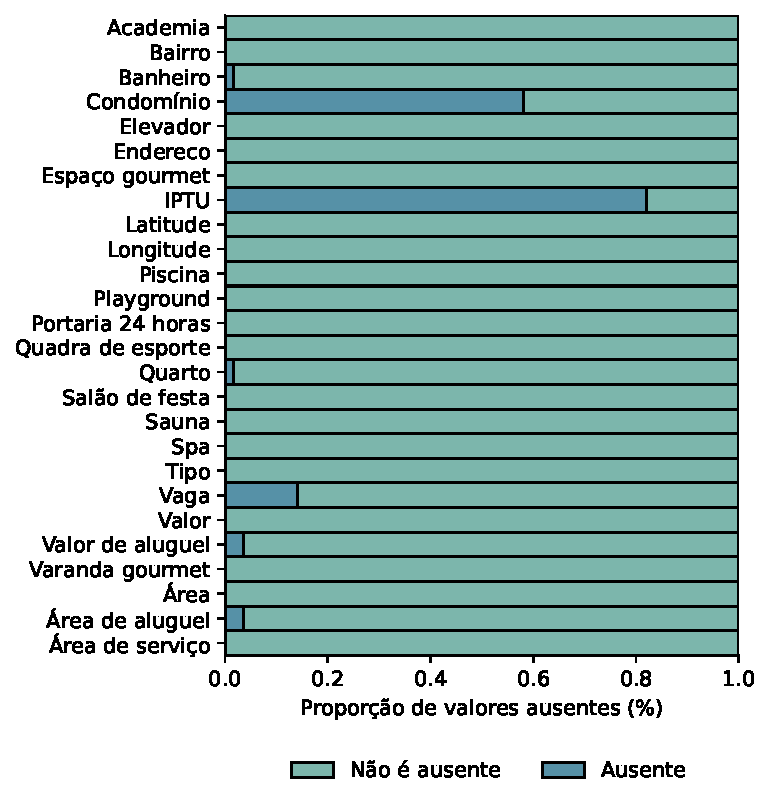
\includegraphics{TCC_files/figure-pdf/fig-miss-output-1.pdf}

}

\caption{\label{fig-miss}Proporção de valores ausentes por variáveis}

\end{figure}%

A primeira etapa da análise exploratória de dados foi identificar os
dados faltantes e determinar a melhor forma de tratá-los. A
Figura~\ref{fig-miss} mostra a porcentagem de observações ausentes em
cada variável. As variáveis com a maior quantidade de dados ausentes são
o valor do condomínio e o IPTU, pois essas informações são as menos
preenchidas no site de onde os dados foram coletados. A terceira
variável, com quase 20\% de observações ausentes, é a quantidade de
vagas de estacionamento. As variáveis com mais de 20\% de observações
ausentes foram removidas da base de dados, pois, com essa quantidade de
valores faltantes, nem mesmo métodos de imputação proporcionariam um
tratamento adequado. Dessa forma, apenas as variáveis de valor do
condomínio e IPTU foram removidas, enquanto as demais com valores
ausentes foram tratadas por meio de imputação.

\vspace{12pt}

Uma das dificuldades que podem surgir durante a modelagem é o
desbalanceamento das classes, ou seja, a diferença na quantidade de cada
tipo de imóvel. O tipo de imóvel mais predominante no conjunto de dados
são os apartamentos, que representam 81,36\% do total. Em seguida, vêm
as casas, com 8,91\%, e os flats, com 5,72\%. Por fim, as casas
comerciais são as menos representadas, com apenas 15 ocorrências. Esse
desbalanceamento claro entre as classes pode dificultar o desempenho do
modelo, especialmente na previsão de categorias menos frequentes, como
as casas comerciais, onde o modelo pode ter dificuldade em obter bons
resultados.

\vspace{12pt}

\begin{figure}

\begin{minipage}{\linewidth}

\centering{

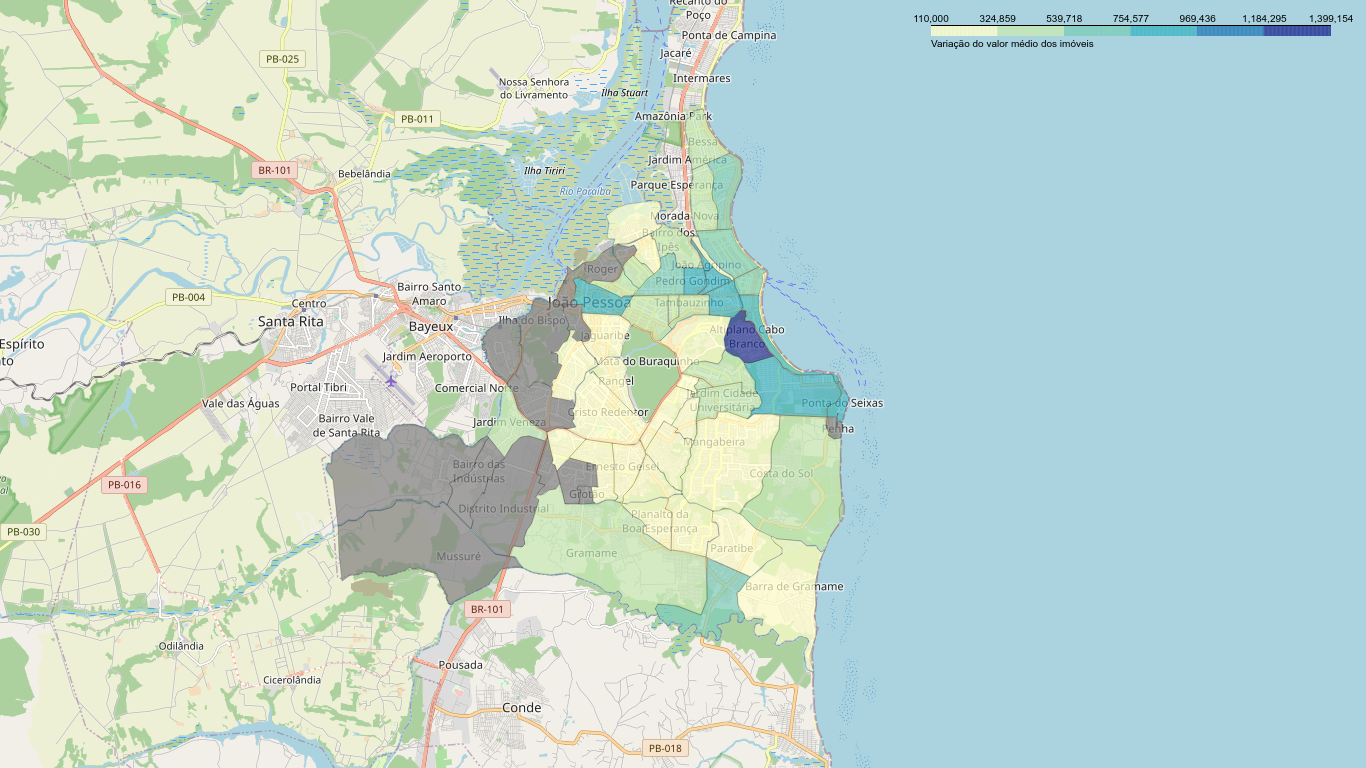
\includegraphics{includes/map_valor_normal.png}

}

\subcaption{\label{fig-mapa_valor}Variação do valor médio dos imóveis.}

\end{minipage}%
\newline
\begin{minipage}{\linewidth}

\centering{

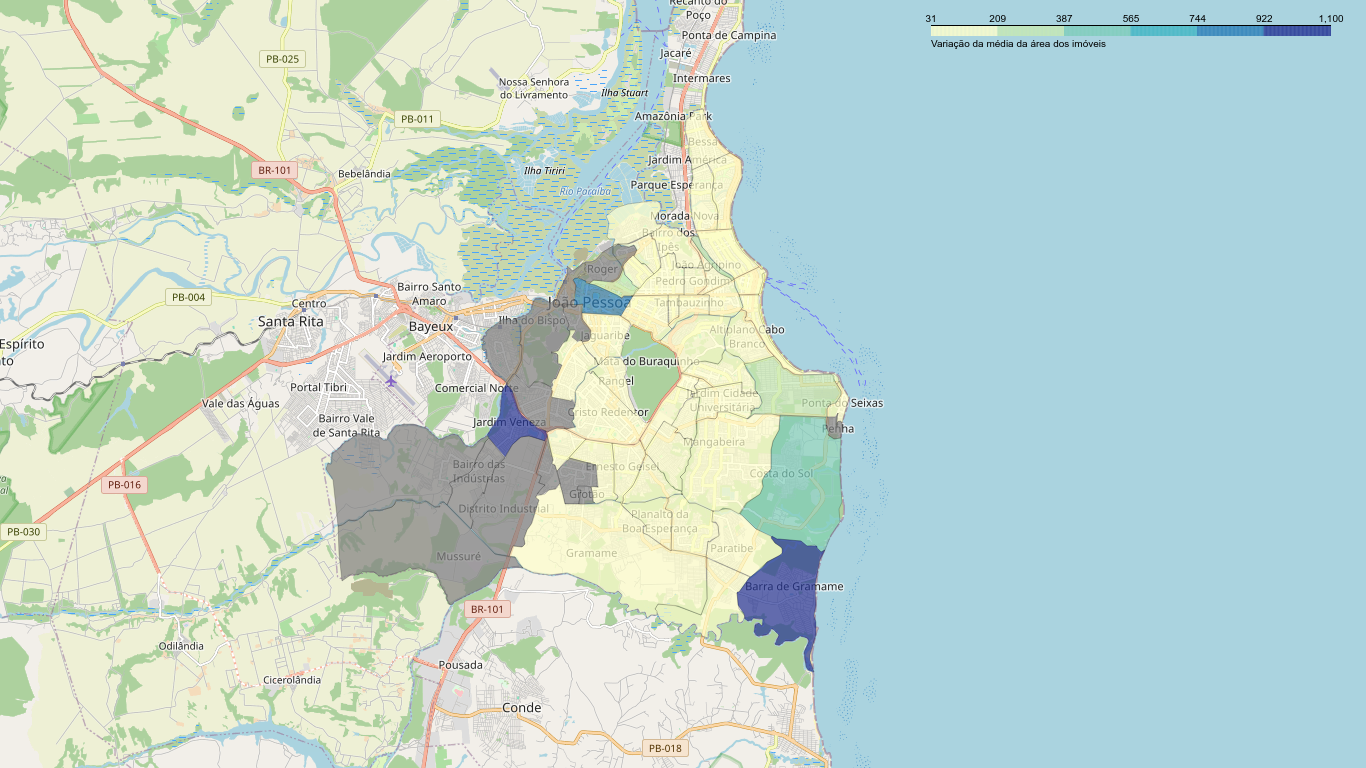
\includegraphics{includes/map_area_normal.png}

}

\subcaption{\label{fig-mapa_area}Variação da média da área dos imóveis.}

\end{minipage}%

\caption{\label{fig-mapas_jp}Mapa da região de João Pessoa, área de
estudo}

\end{figure}%

A partir da Figura~\ref{fig-mapas_jp}, é possível visualizar o mapa da
região de estudo, correspondente à cidade de João Pessoa. O mapa
representado pela Figura~\ref{fig-mapa_valor} exibe a variação da média
do valor dos imóveis, enquanto o mapa Figura~\ref{fig-mapa_area}
apresenta a variação da média da área dos imóveis. Essas variações estão
foram calculadas com base na delimitação dos bairros da cidade de João
Pessoa. Contudo, alguns bairros não possuíam dados no momento da
raspagem de dados e, por isso, estão representados pela cor cinza. Já os
bairros com variação nas cores indicam valores mais altos de áreas ou de
valor dos imóveis conforme as tonalidades se tornam mais escuras. Dessa
forma, observa-se que o bairro com a maior média de valor, aquele que
apresenta a tonalidade mais escura, é o bairro de Altiplano Cabo Branco,
seguido pelo Portal do Sol e em terceiro o bairro de Cabo Branco.

\vspace{12pt}

Embora os bairros de Altiplano Cabo Branco, Portal do sol e Cabo Branco
sejam aqueles com o maior valor são ao mesmo tempo um dos que apresentam
uma das menores áreas médias dos imóveis, como pode ser observado na
Figura~\ref{fig-mapa_area}. O bairro de Barra de Gramame aparece com a
maior área, mas contém apenas um imóvel do tipo terreno com uma área de
1100 \(m^2\), assim como Jardim Veneza que também possuí apenas um
terreno com área de 1050 \(m^2\). O Centro é o bairro com uma das
maiores média de \(m^2\) da cidade de João Pessoa, assim como Costa do
Sol.

\vspace{12pt}

A distribuição das variáveis foram análisadas em termos do tipo do
imóvel a partir de um gráfico de violino. Pela Figura~\ref{fig-violin},
é fácil perceber que a maioria das distribuições possuem assimetria
negativa. Os apartamentos possuem caudas longas à direita, indicando
presença de valores extremamente altos e que indicam que talvez seja
necessário a aplicação de alguma transformação para a estabilização da
variância.

\begin{figure}

\centering{

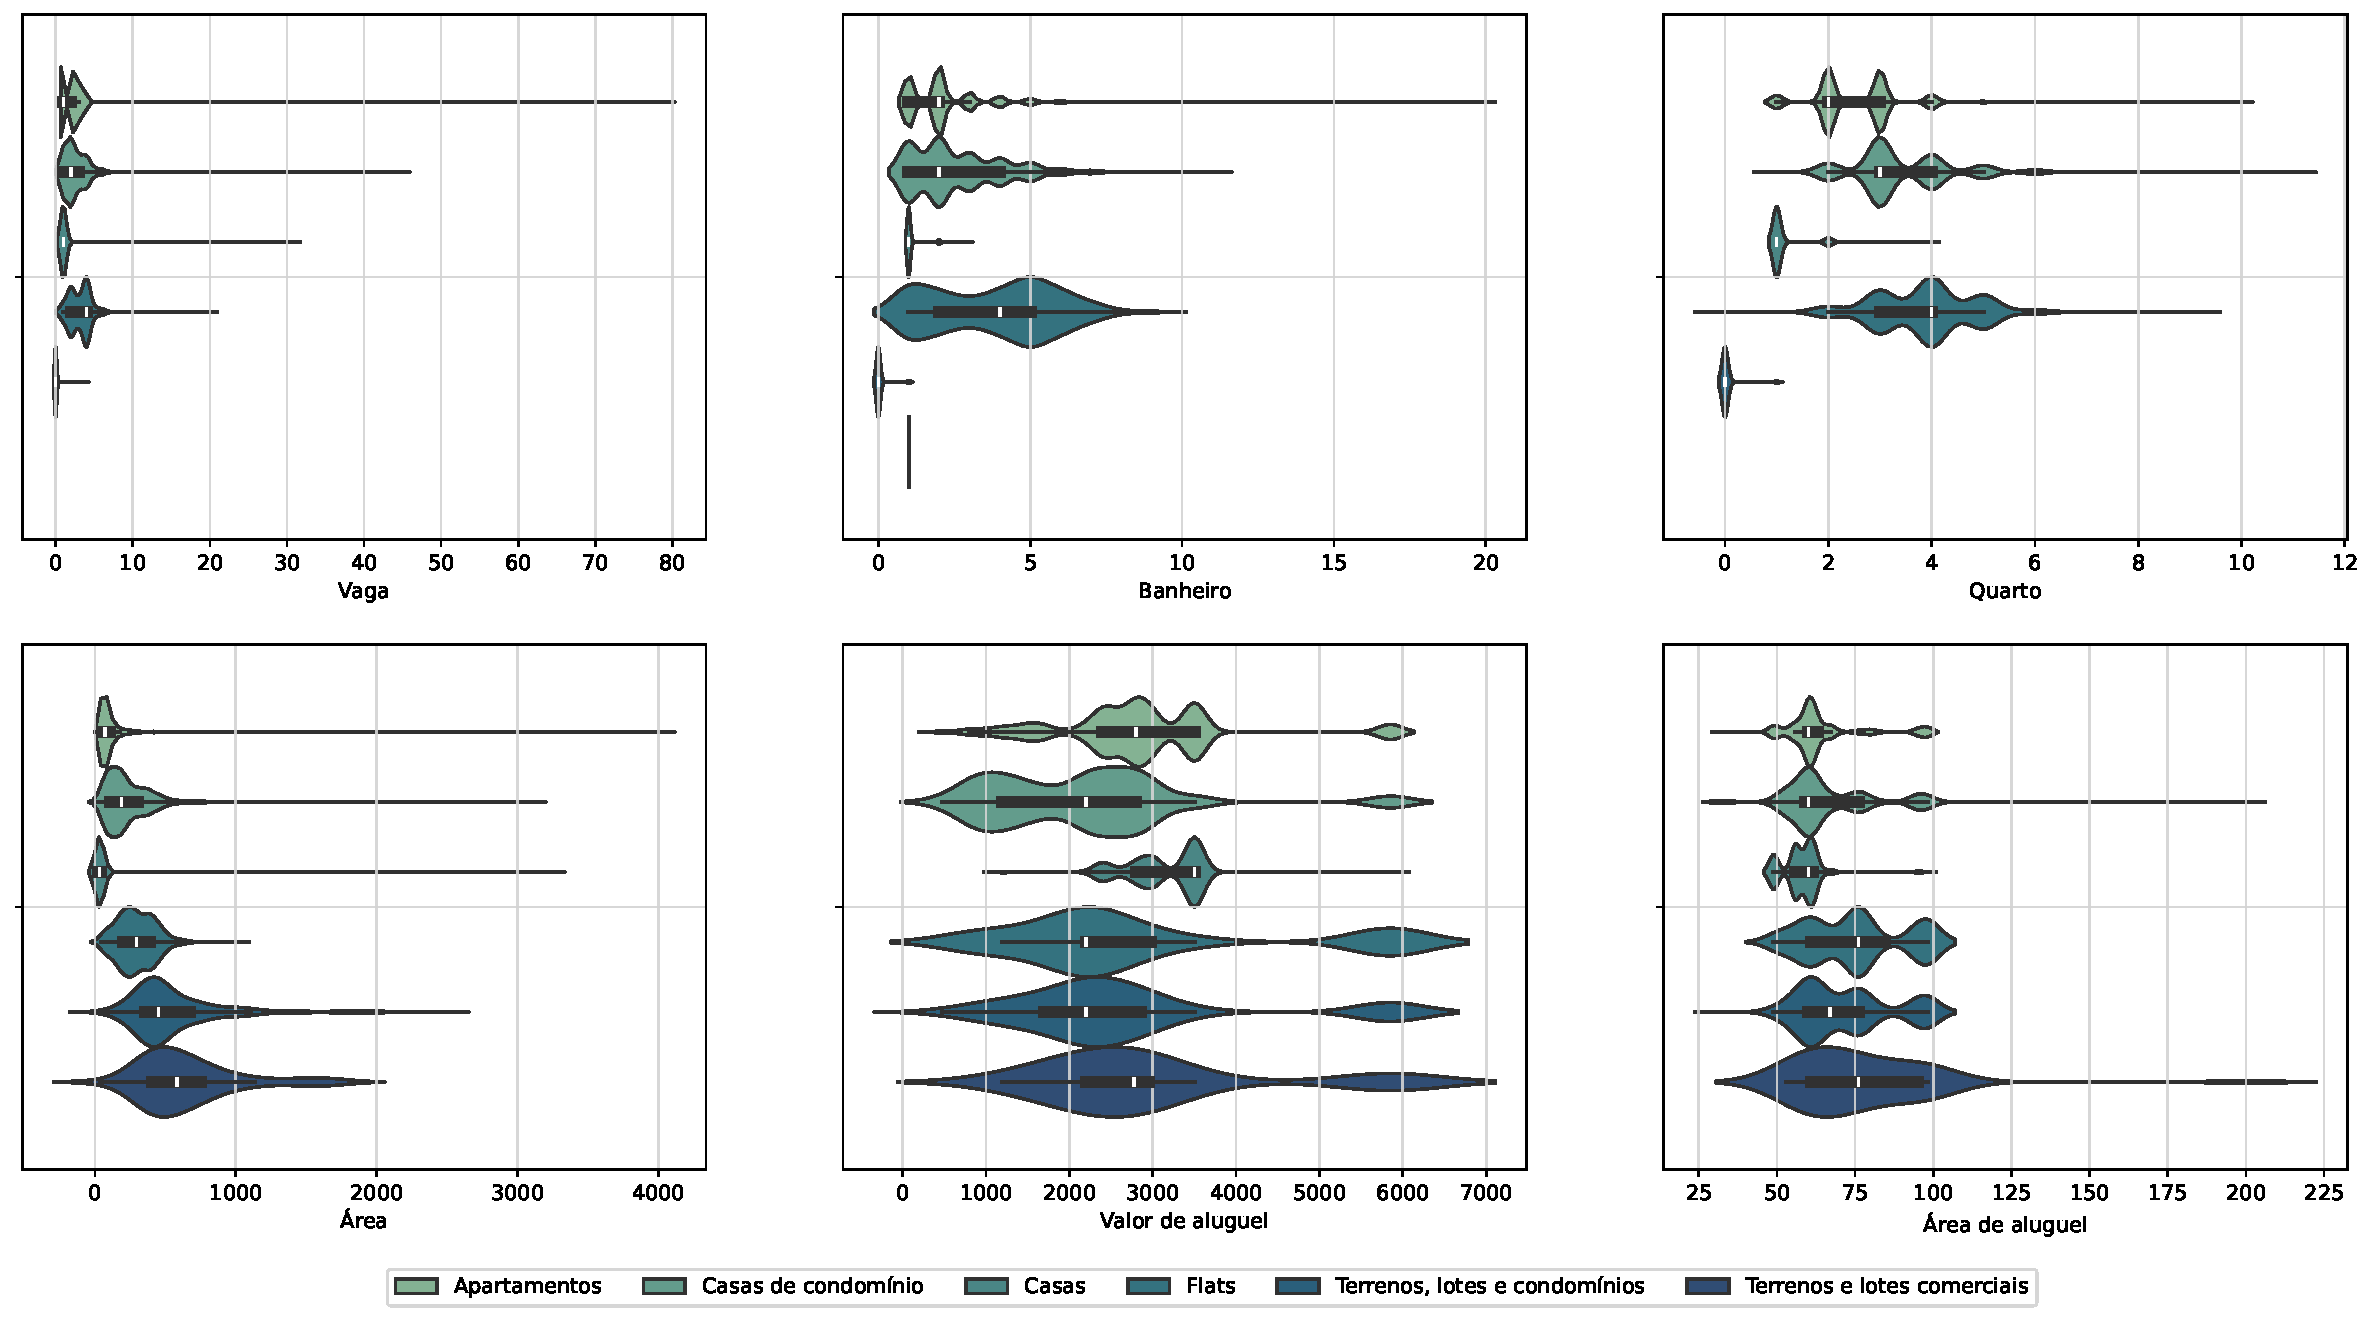
\includegraphics{TCC_files/figure-pdf/fig-violin-output-1.pdf}

}

\caption{\label{fig-violin}Distribuição das variáveis numéricas.}

\end{figure}%

\vspace{12pt}

Para reduzir a assimetria da distribuição dos valores dos imóveis, foi
aplicada uma transformação logarítmica. O gráfico de densidade à
esquerda na Figura~\ref{fig-densitarg} mostra os dados originais da
distribuição do valor dos imóveis. Há uma tendência dos valores ficarem
mais concentrados em uma faixa mais baixa, mas alguns imóveis apresentam
valores excepcionalmente altos, o que acaba gerando uma distribuição
assimétrica positiva. Com a aplicação da transformação logarítmica, a
assimetria é suavizada, comprimindo os valores mais altos. Isso tende a
aproximar a distribuição de uma forma mais simétrica, facilitando a
modelagem e análise estatística.

\begin{figure}

\centering{

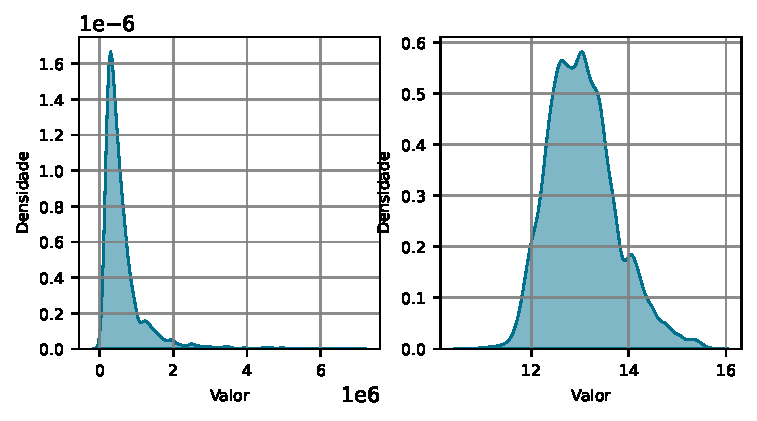
\includegraphics{TCC_files/figure-pdf/fig-densitarg-output-1.pdf}

}

\caption{\label{fig-densitarg}Comparação entre distribuição dos valores
dos imóveis antes e depois da transformação logarítmica.}

\end{figure}%

\begin{figure}

\centering{

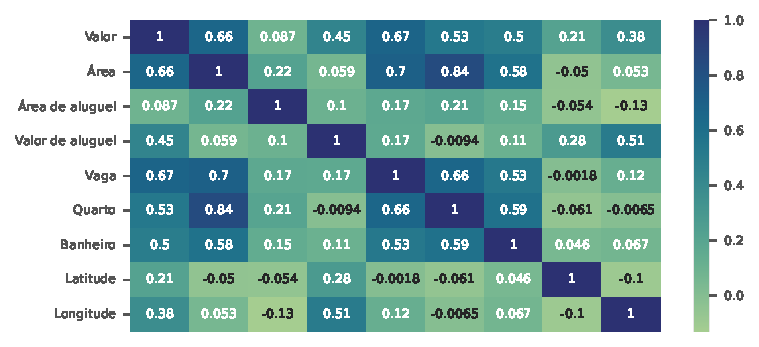
\includegraphics{TCC_files/figure-pdf/fig-corplot-output-1.pdf}

}

\caption{\label{fig-corplot}Gráfico de correlação de Spearman das
variáveis independentes.}

\end{figure}%

\vspace{12pt}

A Figura~\ref{fig-corplot} apresenta a matriz de correlação entre as
variáveis numéricas do conjunto de dados. As cores mais escuras indicam
uma correlação mais forte entre as variáveis, enquanto as cores mais
claras indicam o contrário. O valor do imóvel apresenta maior correlação
com as variáveis de área do imóvel e número de vagas de estacionamento.
Além disso, o valor do imóvel tem alta correlação com o valor médio do
aluguel, número de quartos e banheiros, além de ser fortemente
influenciado pela localização das propriedades. Algumas variáveis
apresentam multicolinearidade entre si, mas os algoritmos utilizados
selecionam aleatoriamente as variáveis para a modelagem, o que reduz o
risco de selecionar variáveis redundantes.

\newpage{}

\section{Tunagem dos modelos}\label{tunagem-dos-modelos}

~~~Como os algoritmos utilizados neste trabalho são baseados em árvores
de decisão ou podem utilizar algoritmos baseados em árvore, como Random
Forest, Gradient Boosting e suas variações, os parâmetros escolhidos
para otimização serão bastantes parecidos. Assim, foram ajustados
hiperparâmetros como o número de árvores e a profundidade das árvores,
de forma a capturar a complexidade das relações presentes nos dados.
Além disso, para os algoritmos baseados em Gradient Boosting, o
hiperparâmetro de taxa de aprendizado também foi ajustado.

\vspace{12pt}

Todos os modelos e bibliotecas usados neste trabalho seguem a API do
scikit-learn. Nessa API, o hiperparâmetro que define a quantidade de
árvores é denominado \texttt{n\_estimators}, o de profundidade das
árvores é \texttt{max\_depth}, e o de taxa de aprendizado é
\texttt{learning\_rate}. Com a configuração da função objetivo na
biblioteca Optuna, foi possível encontrar o ponto ótimo desses
hiperparâmetros para cada modelo. As métricas obtidas para cada
algoritmo pode ser visualizado na Tabela~\ref{tbl-metrics_models}.

\begin{longtable}[]{@{}cccc@{}}
\caption{Métricas obtidadas de cada
algoritmo}\label{tbl-metrics_models}\tabularnewline
\toprule\noalign{}
Algoritmo & RMSE & \(R^2\) & MAPE \\
\midrule\noalign{}
\endfirsthead
\toprule\noalign{}
Algoritmo & RMSE & \(R^2\) & MAPE \\
\midrule\noalign{}
\endhead
\bottomrule\noalign{}
\endlastfoot
Random Forest & 0,28972 & \(86,78792\%\) & 0,01373 \\
Gradient Boosting & 0,28730 & \(86,98259\%\) & 0,01377 \\
Light Gradient Boosting & 0,28493 & \(87,17132\%\) & 0,01346 \\
Extreme Gradient Boosting & 0,28659 & \(87,03891\%\) & 0,01340 \\
Stacking & 0,28473 & \(87,18793\%\) & 0,01357 \\
\end{longtable}

\subsection{Tunagem da Random Forest}\label{tunagem-da-random-forest}

~~~Para o modelo Random Forest, a função objetivo foi definido apenas
para otimizar os hiperparâmetros de quantidade de árvores e de
profundidade da árvore. O espaço de procura para a quantidade de árvores
foi definido entre 1 a 1000 árvores. Já o hiperparâmetro de profundidade
da árvore foi definido entre 20 a 1000. Além disso, foi utilizado
aleatoriamente \(m = \sqrt{p}\) das \(p\) variáveis independentes como
candidatas para a divisão.

\vspace{12pt}

A figura Figura~\ref{fig-rf_slice} mostra a variação da estatística de
erro em função dos valores de cada hiperparâmetro ao longo dos trials. O
gráfico Figura~\ref{fig-rf_import} exibe a importância de cada
hiperparâmetro, calculada pelo método FANOVA. Na figura
Figura~\ref{fig-rf_history}, observa-se a variação do erro para cada
trial, com a linha vermelha representando o menor valor obtido em cada
etapa. Por fim, a figura Figura~\ref{fig-rf_contour} é um gráfico de
área que mostra a interação entre os hiperparâmetros tunados em relação
à estatística de erro.

\vspace{12pt}

A partir de Figura~\ref{fig-rf_slice}, é possível ver que o erro tende a
ser menor para valores menores do hiperparâmetro de profundidade das
árvores (max\_depth). Em contraste, para o hiperparâmetro de número de
árvores (n\_estimators), o erro apresenta uma tendência de redução e
estabilização à medida que o número de árvores aumenta. Esse
comportamento também é observado em Figura~\ref{fig-rf_contour}, onde
valores menores para max\_depth e maiores para n\_estimators resultam em
um modelo com menor erro de generalização.

\vspace{12pt}

Além disso, o gráfico de importância dos hiperparâmetros em
Figura~\ref{fig-rf_import} revela que o hiperparâmetro n\_estimators
possui uma maior contribuição na performance do modelo. A figura
Figura~\ref{fig-rf_history} ilustra o comportamento da métrica de erro
para cada trial, mostrando que o método de otimização alcança um de seus
melhores valores pouco antes do trial 20. Após esse ponto, o otimizador
não consegue encontrar valores de erro significativamente menores.

\begin{figure}

\begin{minipage}{0.50\linewidth}

\centering{

\captionsetup{labelsep=none}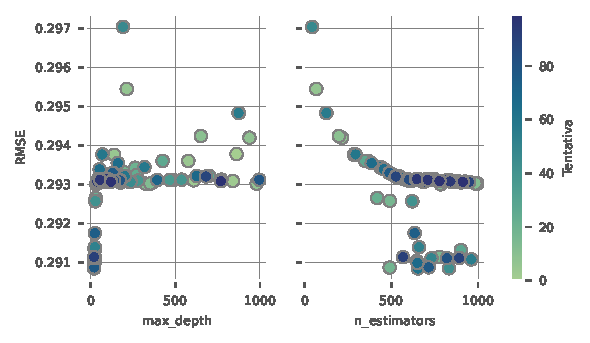
\includegraphics{TCC_files/figure-pdf/fig-rf_slice-output-1.pdf}

}

\subcaption{\label{fig-rf_slice}}

\end{minipage}%
%
\begin{minipage}{0.50\linewidth}

\centering{

\captionsetup{labelsep=none}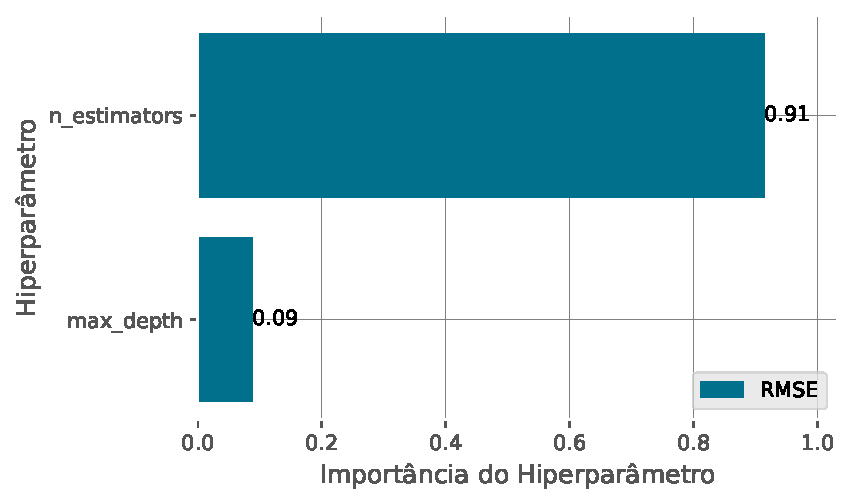
\includegraphics{TCC_files/figure-pdf/fig-rf_import-output-1.pdf}

}

\subcaption{\label{fig-rf_import}}

\end{minipage}%
\newline
\begin{minipage}{0.50\linewidth}

\centering{

\captionsetup{labelsep=none}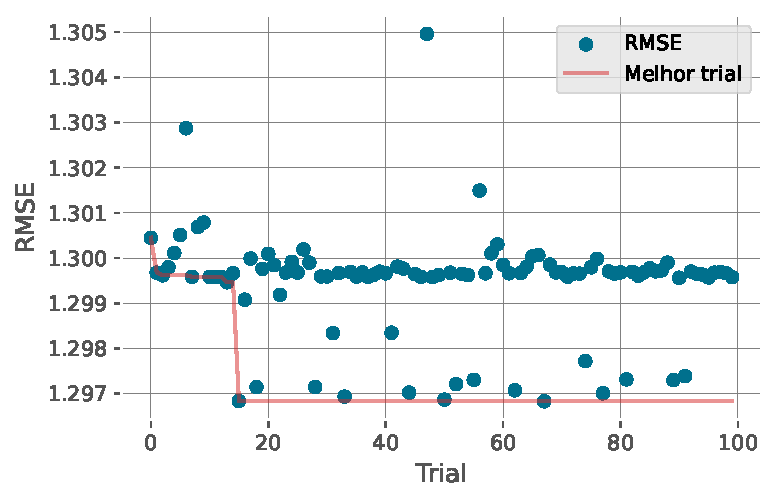
\includegraphics{TCC_files/figure-pdf/fig-rf_history-output-1.pdf}

}

\subcaption{\label{fig-rf_history}}

\end{minipage}%
%
\begin{minipage}{0.50\linewidth}

\centering{

\captionsetup{labelsep=none}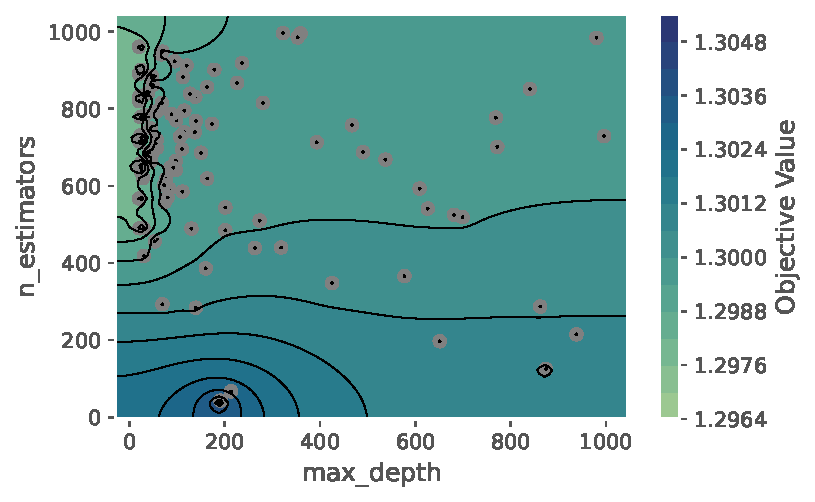
\includegraphics{TCC_files/figure-pdf/fig-rf_contour-output-1.pdf}

}

\subcaption{\label{fig-rf_contour}}

\end{minipage}%

\caption{\label{fig-rf_param}Resultados da tunagem da Random Forest.}

\end{figure}%

\begin{longtable}[]{@{}cccc@{}}
\caption{Melhores hiperparâmetros para Random
Forest}\label{tbl-params_rf}\tabularnewline
\toprule\noalign{}
Tentativa & RMSE & n\_estimators & max\_depth \\
\midrule\noalign{}
\endfirsthead
\toprule\noalign{}
Tentativa & RMSE & n\_estimators & max\_depth \\
\midrule\noalign{}
\endhead
\bottomrule\noalign{}
\endlastfoot
67 & 1,29682 & 650 & 22 \\
\end{longtable}

\subsection{Tunagem do Gradient
Boosting}\label{tunagem-do-gradient-boosting}

~~~Para o algoritmo de Gradient Boosting, os hiperparâmetros ajustados
foram a taxa de aprendizado, a quantidade de árvores e a profundidade
das árvores. No Optuna, o espaço de busca definido na função objetivo
para a taxa de aprendizado variou de \(1 \cdot 10^{-5}\) a
\(1 \cdot 10^{-1}\); para a profundidade das árvores, de 3 a 500; e para
a quantidade de árvores, de 50 a 1500. Assim como no Random Forest, foi
utilizada \(m = \sqrt{p}\)\hspace{0pt} das \(p\) variáveis independentes
para realizar as divisões nas árvores.

\vspace{12pt}

A análise da importância dos hiperparâmetros, apresentada na
Figura~\ref{fig-gdt_import}, indica que o hiperparâmetro com maior
influência na variação da função objetivo --- e, consequentemente, na
performance do modelo --- é a taxa de aprendizado. Em seguida, a
profundidade das árvores é o segundo mais relevante, enquanto o número
de árvores tem a menor influência.

\begin{figure}

\begin{minipage}{0.33\linewidth}

\centering{

\captionsetup{labelsep=none}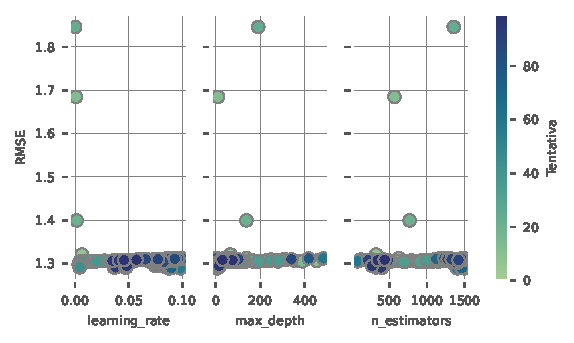
\includegraphics{TCC_files/figure-pdf/fig-gdt_slice-output-1.pdf}

}

\subcaption{\label{fig-gdt_slice}}

\end{minipage}%
%
\begin{minipage}{0.33\linewidth}

\centering{

\captionsetup{labelsep=none}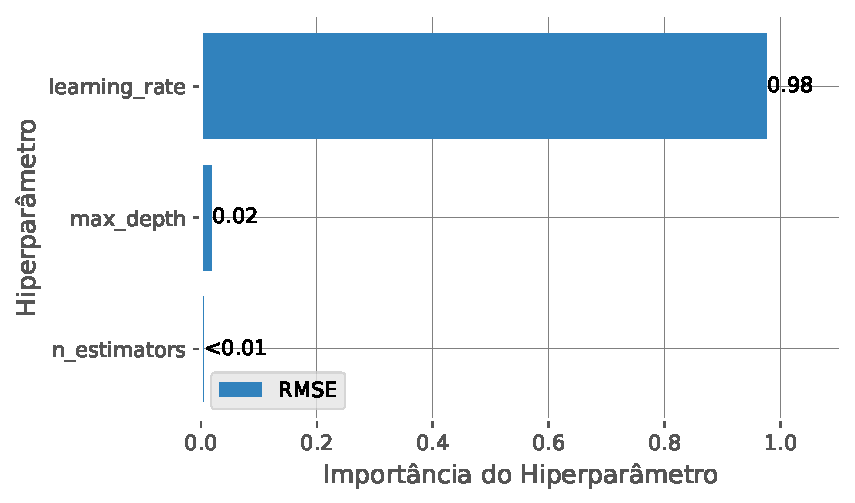
\includegraphics{TCC_files/figure-pdf/fig-gdt_import-output-1.pdf}

}

\subcaption{\label{fig-gdt_import}}

\end{minipage}%
%
\begin{minipage}{0.33\linewidth}

\centering{

\captionsetup{labelsep=none}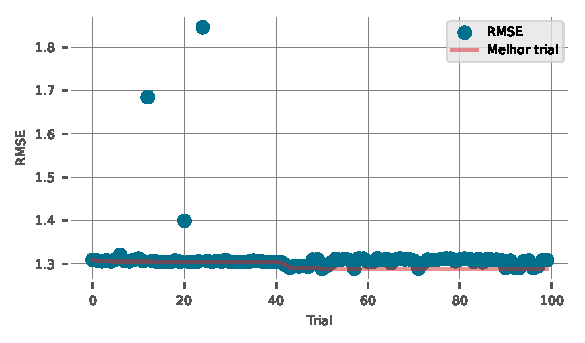
\includegraphics{TCC_files/figure-pdf/fig-gdt_history-output-1.pdf}

}

\subcaption{\label{fig-gdt_history}}

\end{minipage}%
\newline
\begin{minipage}{\linewidth}

\centering{

\captionsetup{labelsep=none}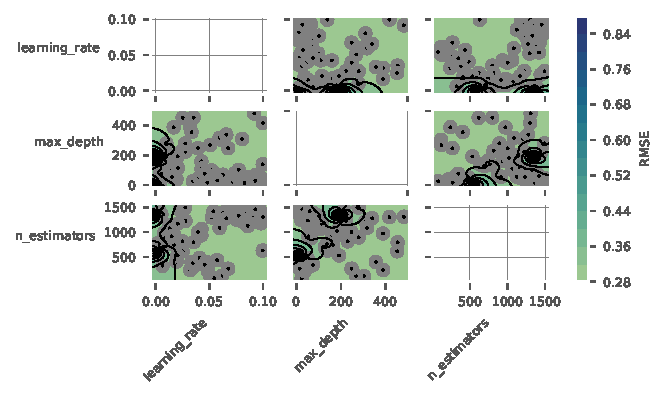
\includegraphics{TCC_files/figure-pdf/fig-gdt_contour-output-1.pdf}

}

\subcaption{\label{fig-gdt_contour}}

\end{minipage}%

\caption{\label{fig-gdt_param}Resultados da tunagem do Gradient
Boosting}

\end{figure}%

Diferentemente do modelo de Random Forest, o algoritmo de Gradient
Boosting não apresentou melhorias significativas, como ilustrado na
Figura~\ref{fig-gdt_history}, onde a estatística de erro poucas vezes
ficou abaixo de 1,3. A relação entre os hiperparâmetros é bastante
similar à obtida para o Random Forest. Na Figura~\ref{fig-gdt_contour},
observa-se que o método de otimização TPE tende a selecionar valores
menores para a profundidade das árvores e maiores para o número de
árvores. No entanto, também há uma preferência por uma menor quantidade
de árvores quando a taxa de aprendizado diminui.

\begin{longtable}[]{@{}ccccc@{}}
\caption{Melhores hiperparâmetros para Gradient
Boosting}\label{tbl-params_gdt}\tabularnewline
\toprule\noalign{}
Tentativa & RMSE & n\_estimators & max\_depth & learning\_rate \\
\midrule\noalign{}
\endfirsthead
\toprule\noalign{}
Tentativa & RMSE & n\_estimators & max\_depth & learning\_rate \\
\midrule\noalign{}
\endhead
\bottomrule\noalign{}
\endlastfoot
50 & 1,28891 & 1500 & 6 & 0,08730 \\
\end{longtable}

\subsection{Tunagem do LGBM}\label{tunagem-do-lgbm}

~~~Para a otimização do LGBM, foram considerados os mesmos
hiperparâmetros do algoritmo de Gradient Boosting, mas agora também com
a tunagem do número de folhas das árvores. O espaço de busca para a
quantidade de árvores foi definido entre 100 e 2000, para a taxa de
aprendizado no mesmo intervalo usado no Gradient Boosting, para a
profundidade das árvores e número de folhas o intervalo foi definido da
mesma forma, entre 100 e 500

\begin{figure}

\begin{minipage}{0.33\linewidth}

\centering{

\captionsetup{labelsep=none}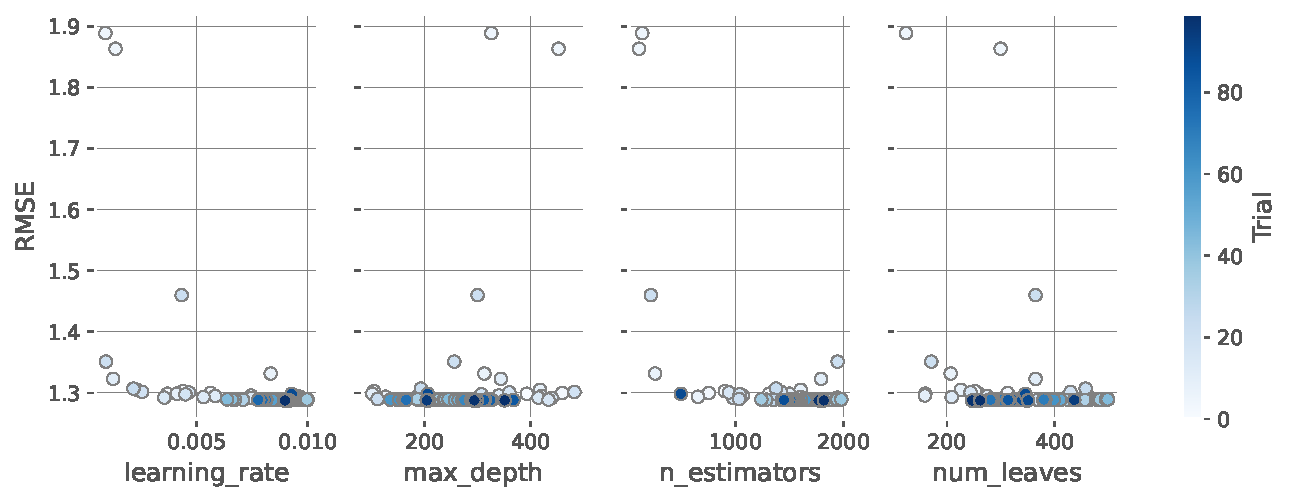
\includegraphics{TCC_files/figure-pdf/fig-lgbm_slice-output-1.pdf}

}

\subcaption{\label{fig-lgbm_slice}}

\end{minipage}%
%
\begin{minipage}{0.33\linewidth}

\centering{

\captionsetup{labelsep=none}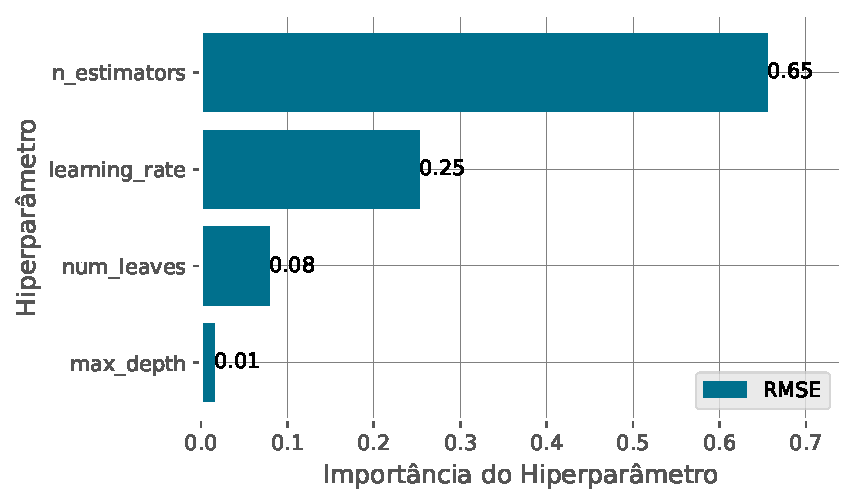
\includegraphics{TCC_files/figure-pdf/fig-lgbm_import-output-1.pdf}

}

\subcaption{\label{fig-lgbm_import}}

\end{minipage}%
%
\begin{minipage}{0.33\linewidth}

\centering{

\captionsetup{labelsep=none}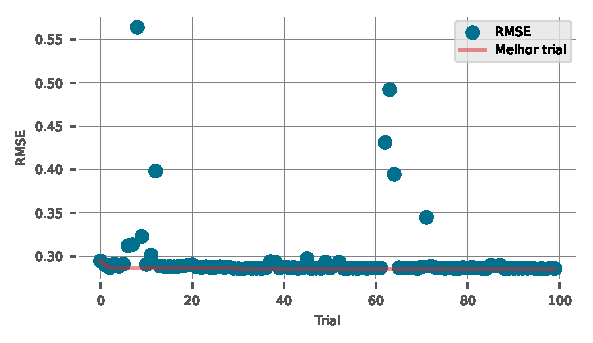
\includegraphics{TCC_files/figure-pdf/fig-lgbm_history-output-1.pdf}

}

\subcaption{\label{fig-lgbm_history}}

\end{minipage}%
\newline
\begin{minipage}{\linewidth}

\centering{

\captionsetup{labelsep=none}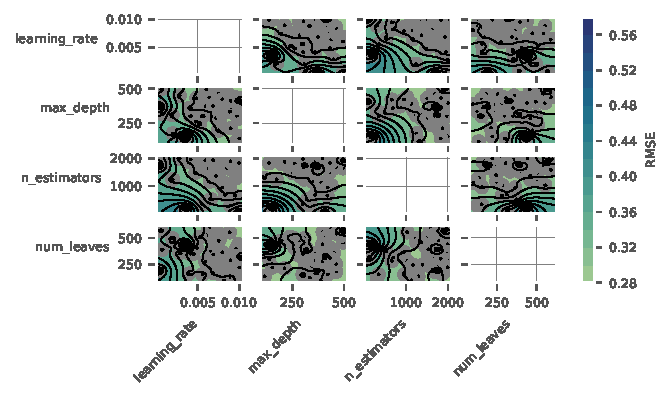
\includegraphics{TCC_files/figure-pdf/fig-lgbm_contour-output-1.pdf}

}

\subcaption{\label{fig-lgbm_contour}}

\end{minipage}%

\caption{\label{fig-lgbm_param}Resultados da tunagem do LGBM}

\end{figure}%

\vspace{12pt}

As trials de otimização do modelo LGBM (Figura~\ref{fig-lgbm_history})
apresentaram um comportamento semelhante ao do Gradient Boosting, porém
com maior estabilidade em cada tentativa e uma convergência mais rápida.
Ao analisar a contribuição de cada hiperparâmetro para o desempenho do
modelo na Figura~\ref{fig-lgbm_import}, observa-se que a quantidade de
árvores é o hiperparâmetro de maior influência, seguido pela taxa de
aprendizado, número de folhas e, por último, a profundidade da árvore.

\vspace{12pt}

Analisando a relação entre o hiperparâmetro de profundidade e o número
de folhas em função da estatística de erro na
Figura~\ref{fig-lgbm_contour}, observa-se que uma maior quantidade de
folhas e uma menor profundidade das árvores resultam em um modelo com
erro menor. Esse mesmo comportamento é observado para os outros
hiperparâmetros, uma quantidade maior de folhas combinada com uma taxa
de aprendizado crescente também produz um modelo com menor erro, assim
como um número maior de árvores.

\begin{longtable}[]{@{}
  >{\centering\arraybackslash}p{(\columnwidth - 10\tabcolsep) * \real{0.1549}}
  >{\centering\arraybackslash}p{(\columnwidth - 10\tabcolsep) * \real{0.1127}}
  >{\centering\arraybackslash}p{(\columnwidth - 10\tabcolsep) * \real{0.1972}}
  >{\centering\arraybackslash}p{(\columnwidth - 10\tabcolsep) * \real{0.1690}}
  >{\centering\arraybackslash}p{(\columnwidth - 10\tabcolsep) * \real{0.1549}}
  >{\centering\arraybackslash}p{(\columnwidth - 10\tabcolsep) * \real{0.2113}}@{}}
\caption{Melhores hiperparâmetros para Light Gradient
Boosting}\label{tbl-params_lgbm}\tabularnewline
\toprule\noalign{}
\begin{minipage}[b]{\linewidth}\centering
Tentativa
\end{minipage} & \begin{minipage}[b]{\linewidth}\centering
RMSE
\end{minipage} & \begin{minipage}[b]{\linewidth}\centering
n\_estimators
\end{minipage} & \begin{minipage}[b]{\linewidth}\centering
num\_leaves
\end{minipage} & \begin{minipage}[b]{\linewidth}\centering
max\_depth
\end{minipage} & \begin{minipage}[b]{\linewidth}\centering
learning\_rate
\end{minipage} \\
\midrule\noalign{}
\endfirsthead
\toprule\noalign{}
\begin{minipage}[b]{\linewidth}\centering
Tentativa
\end{minipage} & \begin{minipage}[b]{\linewidth}\centering
RMSE
\end{minipage} & \begin{minipage}[b]{\linewidth}\centering
n\_estimators
\end{minipage} & \begin{minipage}[b]{\linewidth}\centering
num\_leaves
\end{minipage} & \begin{minipage}[b]{\linewidth}\centering
max\_depth
\end{minipage} & \begin{minipage}[b]{\linewidth}\centering
learning\_rate
\end{minipage} \\
\midrule\noalign{}
\endhead
\bottomrule\noalign{}
\endlastfoot
96 & 1,28722 & 1798 & 247 & 299 & 0,00903 \\
\end{longtable}

\subsection{Tunagem do XGBoost}\label{tunagem-do-xgboost}

~~~Para o algoritmo Extreme Gradient Boosting, os hiperparâmetros
selecionados para a tunagem foi a taxa de aprendizagem, profundidade da
árvore e quantidade máxima de árvores. Na configuração da função
objetivo para a tunagem dos hiperparâmetros pelo optuna, a taxa de
aprendizagem variou entre \(1 \cdot 10^{-7}\) e \(0.5\), a profundidade
da árvore variou entre 3 e 50 e a quantidade de árvores variou entre 50
e 1000.

\vspace{12pt}

A partir da Figura~\ref{fig-xgb_import}, o hiperparâmetro que
representou a maior variação na função objetivo, e portanto a maior
importância para a performance do modelo, foi a taxa de aprendizagem. A
profundidade da árvore representou 22\% da variação e por último vem a
quantidade de árvores. Observando a Figura~\ref{fig-xgb_history}, é
possível ver que o algoritmo de XGBoost foi aquele que apresentou a
menor variação entre os trials, com um único trial com erro acima de
2,0.

\vspace{12pt}

O algoritmo de otimização TPE apresentou uma maior frequência de procura
do hiperparâmetro de taxa de aprendizagem para valores menores, como
pode ser visto na Figura~\ref{fig-xgb_slice}. O mesmo acontece para o
hiperparâmetro de profundidade de árvores, há uma repetição maior para
valores menores, indicando que o a estatística de erro tendeu a ter
valores menores para essa região. Para a quantidade de árvores esse
padrão foi diferente, uma quantidade maior de árvores faz com que o
modelo tenha um melhor ajuste. Essas relações também podem ser
observadas a partir da Figura~\ref{fig-xgb_contour}, menores taxas de
aprendizado, combinado com uma menor profundidade de árvore e maior
quantidade de árvores apresentam menor valor na função objetivo.

\begin{figure}

\begin{minipage}{0.33\linewidth}

\centering{

\captionsetup{labelsep=none}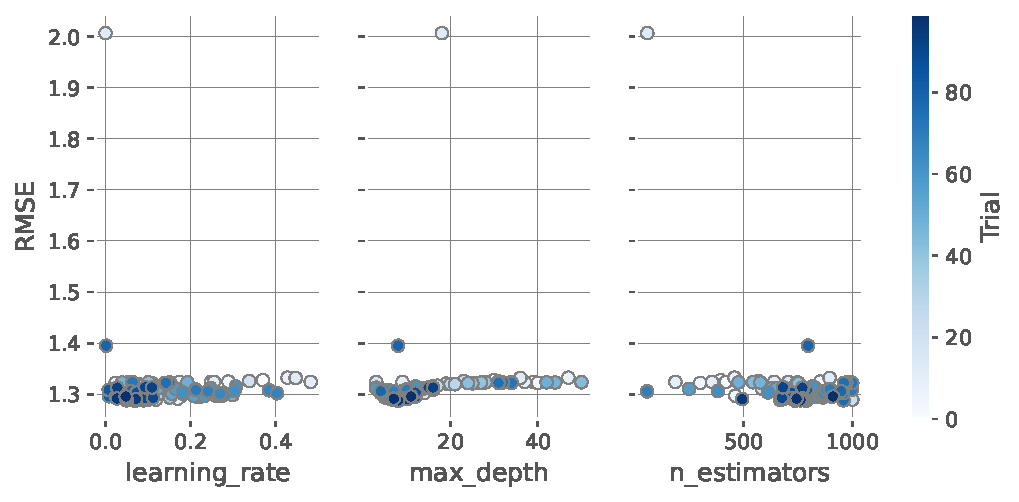
\includegraphics{TCC_files/figure-pdf/fig-xgb_slice-output-1.pdf}

}

\subcaption{\label{fig-xgb_slice}}

\end{minipage}%
%
\begin{minipage}{0.33\linewidth}

\centering{

\captionsetup{labelsep=none}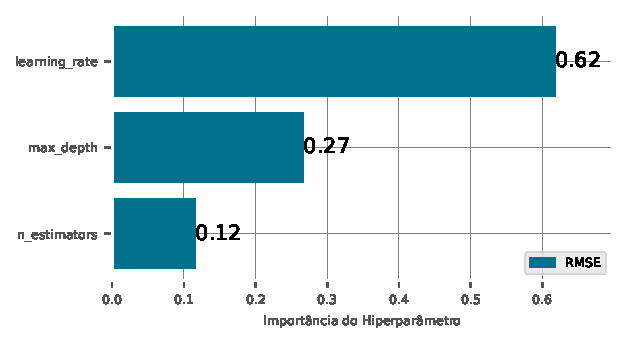
\includegraphics{TCC_files/figure-pdf/fig-xgb_import-output-1.pdf}

}

\subcaption{\label{fig-xgb_import}}

\end{minipage}%
%
\begin{minipage}{0.33\linewidth}

\centering{

\captionsetup{labelsep=none}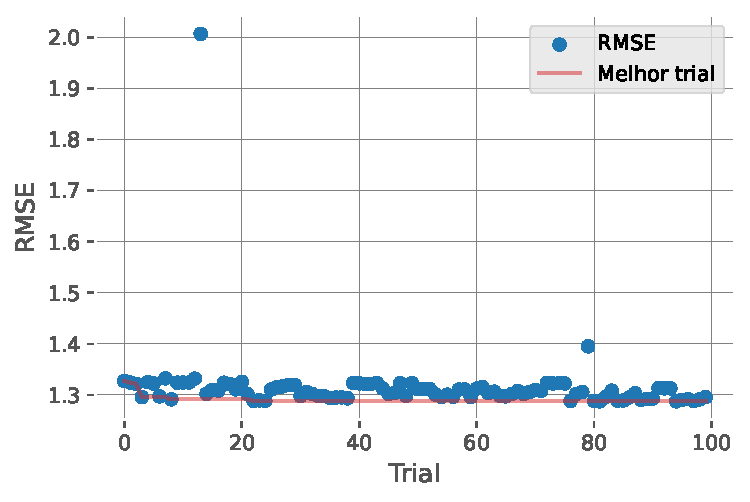
\includegraphics{TCC_files/figure-pdf/fig-xgb_history-output-1.pdf}

}

\subcaption{\label{fig-xgb_history}}

\end{minipage}%
\newline
\begin{minipage}{\linewidth}

\centering{

\captionsetup{labelsep=none}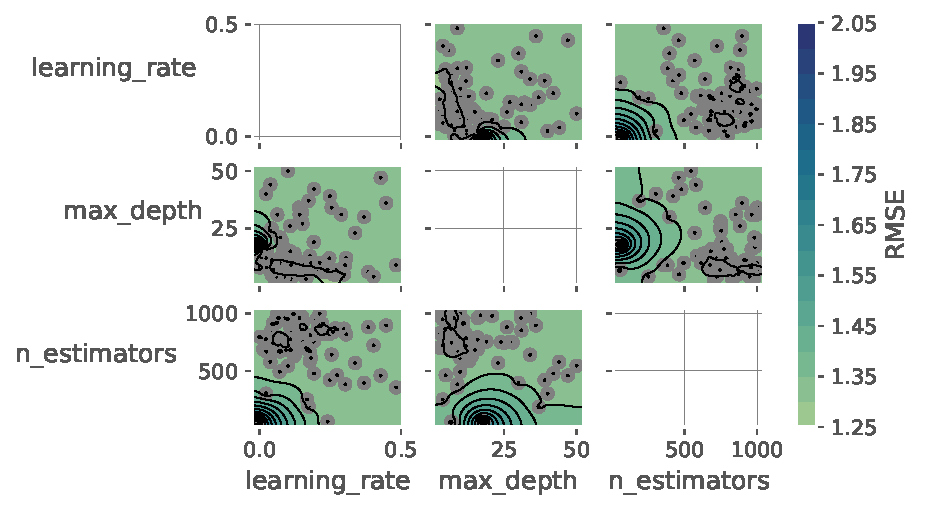
\includegraphics{TCC_files/figure-pdf/fig-xgb_contour-output-1.pdf}

}

\subcaption{\label{fig-xgb_contour}}

\end{minipage}%

\caption{\label{fig-xgb_param}Resultados da tunagem do XGBoost}

\end{figure}%

\begin{longtable}[]{@{}ccccc@{}}
\caption{Melhores hiperparâmetros para Extreme Gradient
Boosting}\label{tbl-params_xgb}\tabularnewline
\toprule\noalign{}
Tentativa & RMSE & n\_estimators & max\_depth & learning\_rate \\
\midrule\noalign{}
\endfirsthead
\toprule\noalign{}
Tentativa & RMSE & n\_estimators & max\_depth & learning\_rate \\
\midrule\noalign{}
\endhead
\bottomrule\noalign{}
\endlastfoot
81 & 1,28752 & 788 & 8 & 0,07119 \\
\end{longtable}

A tabela Tabela~\ref{tbl-params_xgb} apresenta a tentativa em que a
combinação de hiperparâmetros resultou no menor erro para o algoritmo de
Extreme Gradient Boosting. Nesse caso, a melhor tentativa foi a de
número 81, com uma configuração de 788 árvores, profundidade máxima de 8
e taxa de aprendizado de 0,07119.

\vspace{12pt}

Para o LGBM, a melhor combinação foi encontrada na tentativa 96, com
1.798 árvores, 247 folhas, profundidade máxima de 299 e taxa de
aprendizado de 0,00903, como apresentado na tabela
Tabela~\ref{tbl-params_lgbm}.

\vspace{12pt}

Por fim, para os algoritmos Gradient Boosting e Random Forest, as
melhores tentativas foram as de números 50 e 67, respectivamente. No
caso do Gradient Boosting, a configuração ideal foi composta por 1.500
árvores, profundidade máxima de 6 e taxa de aprendizado de 0,08730. Já
para o Random Forest, a melhor combinação consistiu em 650 árvores e
profundidade máxima de 22. Os resultados estão na
Tabela~\ref{tbl-params_gdt} e Tabela~\ref{tbl-params_rf},
respectivamente.

\section{Resultados dos modelos}\label{resultados-dos-modelos}

~~~Nesta seção, serão apresentados os resultados do ajuste de cada
algoritmo utilizado: Random Forest, Gradient Boosting, LightGBM e
Extreme Gradient Boosting. A análise do ajuste foi realizada com base no
gráfico que compara os valores estimados aos valores observados dos
imóveis. Além disso, foram utilizadas métricas de erro, como MAPE,
\(R^2\) e RMSE, para avaliar o desempenho dos modelos.

\vspace{12pt}

O ajuste do algoritmo Random Forest é apresentado na figura
Figura~\ref{fig-preds_rf}, que exibe a comparação entre os valores
previstos e observados. Em termos da transformação logarítmica
realizada, a raiz do erro quadrático médio (RMSE) foi de 0,28972,
enquanto o coeficiente de determinação \(R^2\) alcançou \(86,79%
\), indicando que o modelo explica \(86,79%
\) da variação dos dados. Em relação ao MAPE, o valor foi de 0,01373,
assim, em média, as predições realizadas pelo modelo Random Forest,
considerando a transformação logarítmica, estiveram 1,373\% distantes
dos valores reais.

\vspace{12pt}

Em relação ao algoritmo de Gradient Boosting, o seu ajuste consegue
explicar \(86,98\%\) dos dados, bastante semelhante à Random Forest, com
uma diferença não tão significativa. Por outro lado, o RMSE do Gradient
Boosting foi menor que a Random Forest, tendo sido de 0,28730.
Observando o MAPE, não houve também muitas diferenças, embora o MAPE do
Gradient Boosting tenha sido maior. O MAPE indica que as predições
geradas pelo Gradient Boosting estão \(1,377\%\) distantes de seus
valores observados. Seu ajuste pode ser observado na
Figura~\ref{fig-preds_gdt}.

\begin{figure}

\begin{minipage}{0.50\linewidth}

\centering{

\captionsetup{labelsep=none}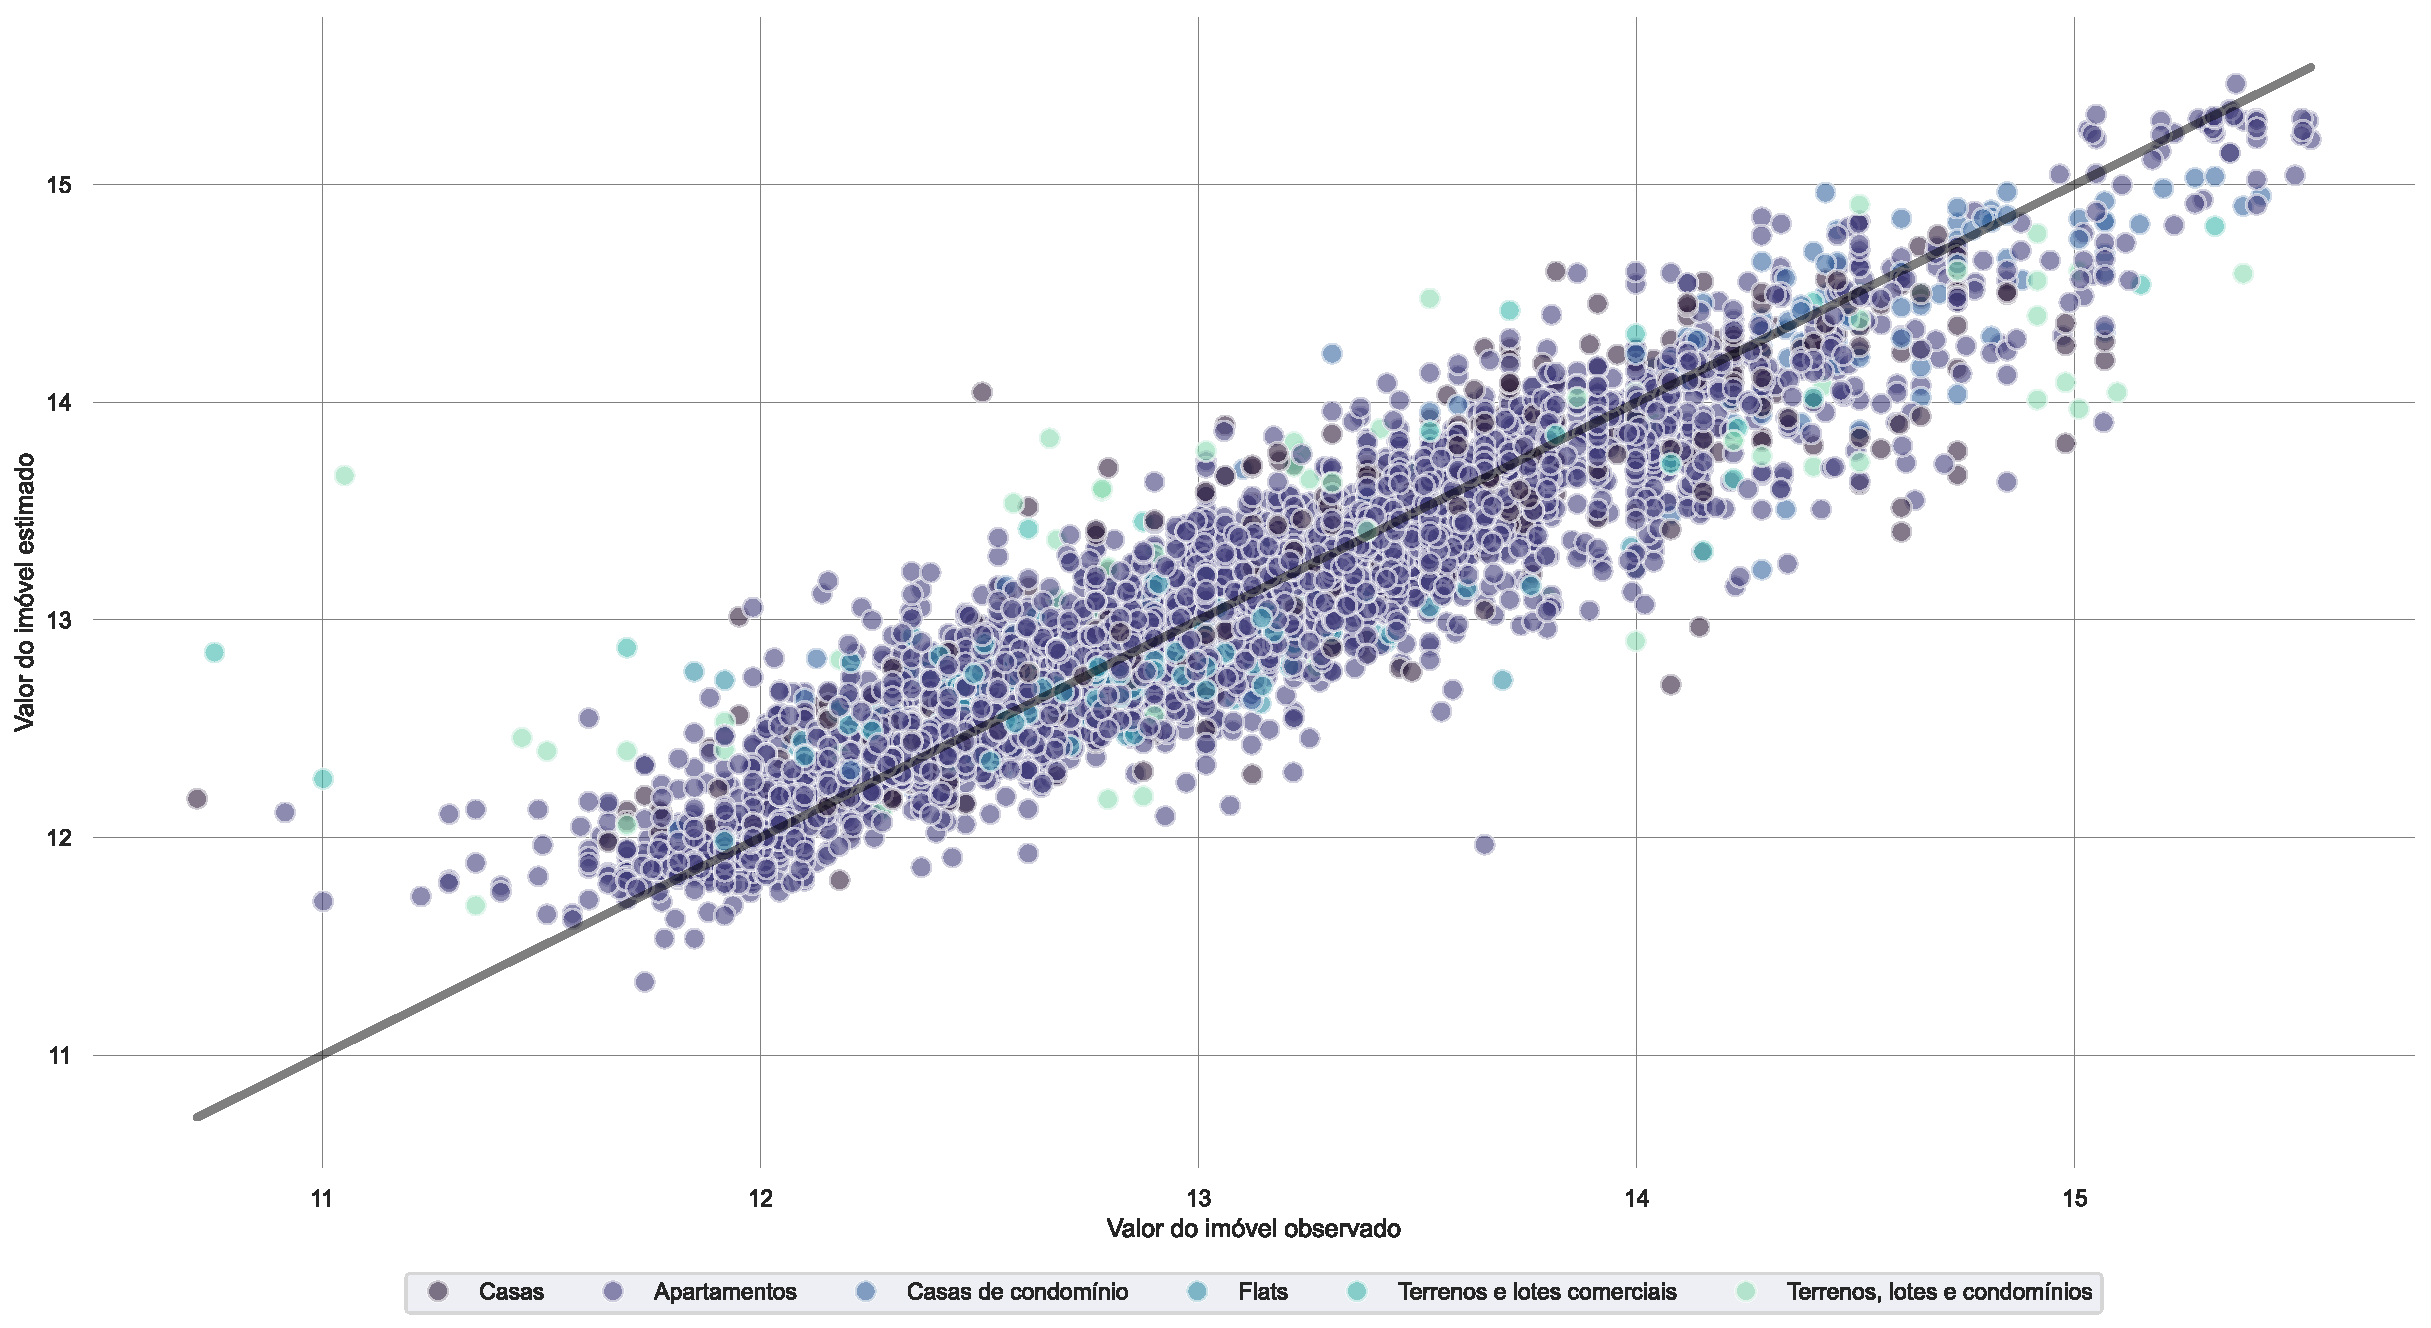
\includegraphics{TCC_files/mediabag/includes/rf_plot_predict.pdf}

}

\subcaption{\label{fig-preds_rf}}

\end{minipage}%
%
\begin{minipage}{0.50\linewidth}

\centering{

\captionsetup{labelsep=none}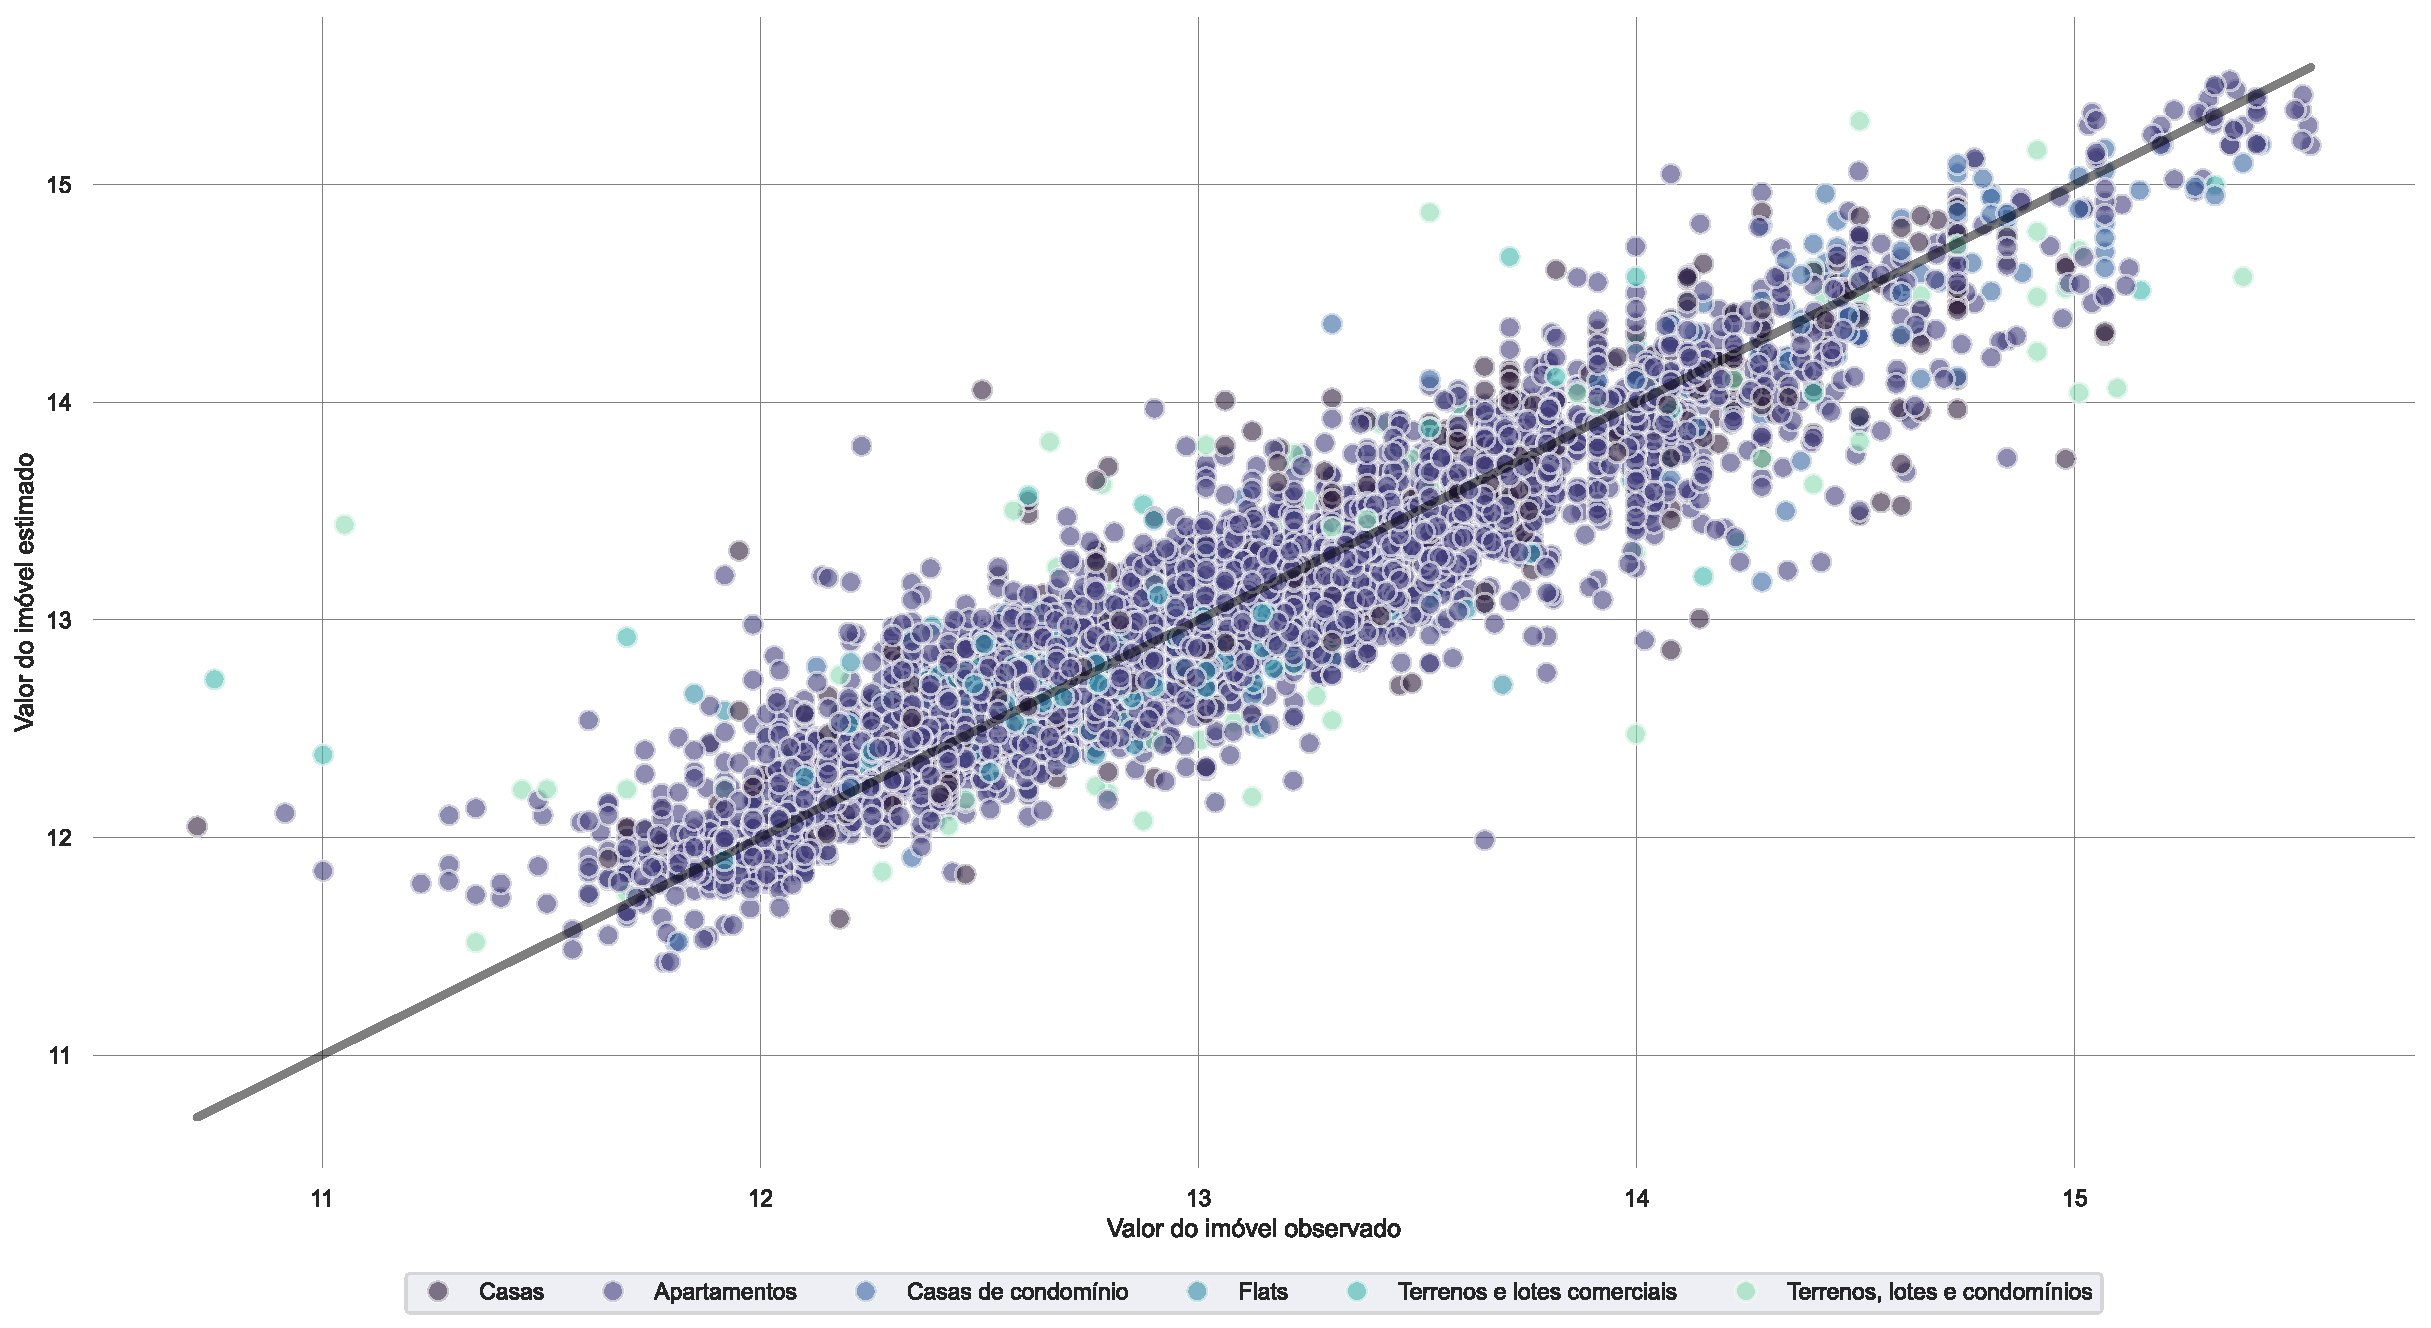
\includegraphics{TCC_files/mediabag/includes/gdt_plot_predict.pdf}

}

\subcaption{\label{fig-preds_gdt}}

\end{minipage}%

\caption{\label{fig-preds1}Valores previstos em função dos observados do
algoritmo Random Forest e Gradient Boosting, respectivamente.}

\end{figure}%

\vspace{12pt}

O Light Gradient Boosting conseguiu melhorias em relação aos resultados
dos últimos dois algoritmos. Em relação ao seu \(R^2\), o modelo
consegue explicar \(87,17\%\) dos dados. O seu RMSE ficou em \(0,28493\)
e o MAPE em \(0,01346\). Dessa forma, as predições geradas pelo Light
Gradient Boosting estão em média \(1,346\%\) distantes de seus valores
reais. A melhora do ajuste do Light Gradient Boosting fica bastante
perceptível observando a figura de seus valores estimados em função dos
observados (Figura~\ref{fig-preds_lgbm}). As predições geradas pelos
Gradient Boosting e Random Forest desviam bastante, principalmente em
relação ao final da distribuição.

\begin{figure}

\begin{minipage}{0.50\linewidth}

\centering{

\captionsetup{labelsep=none}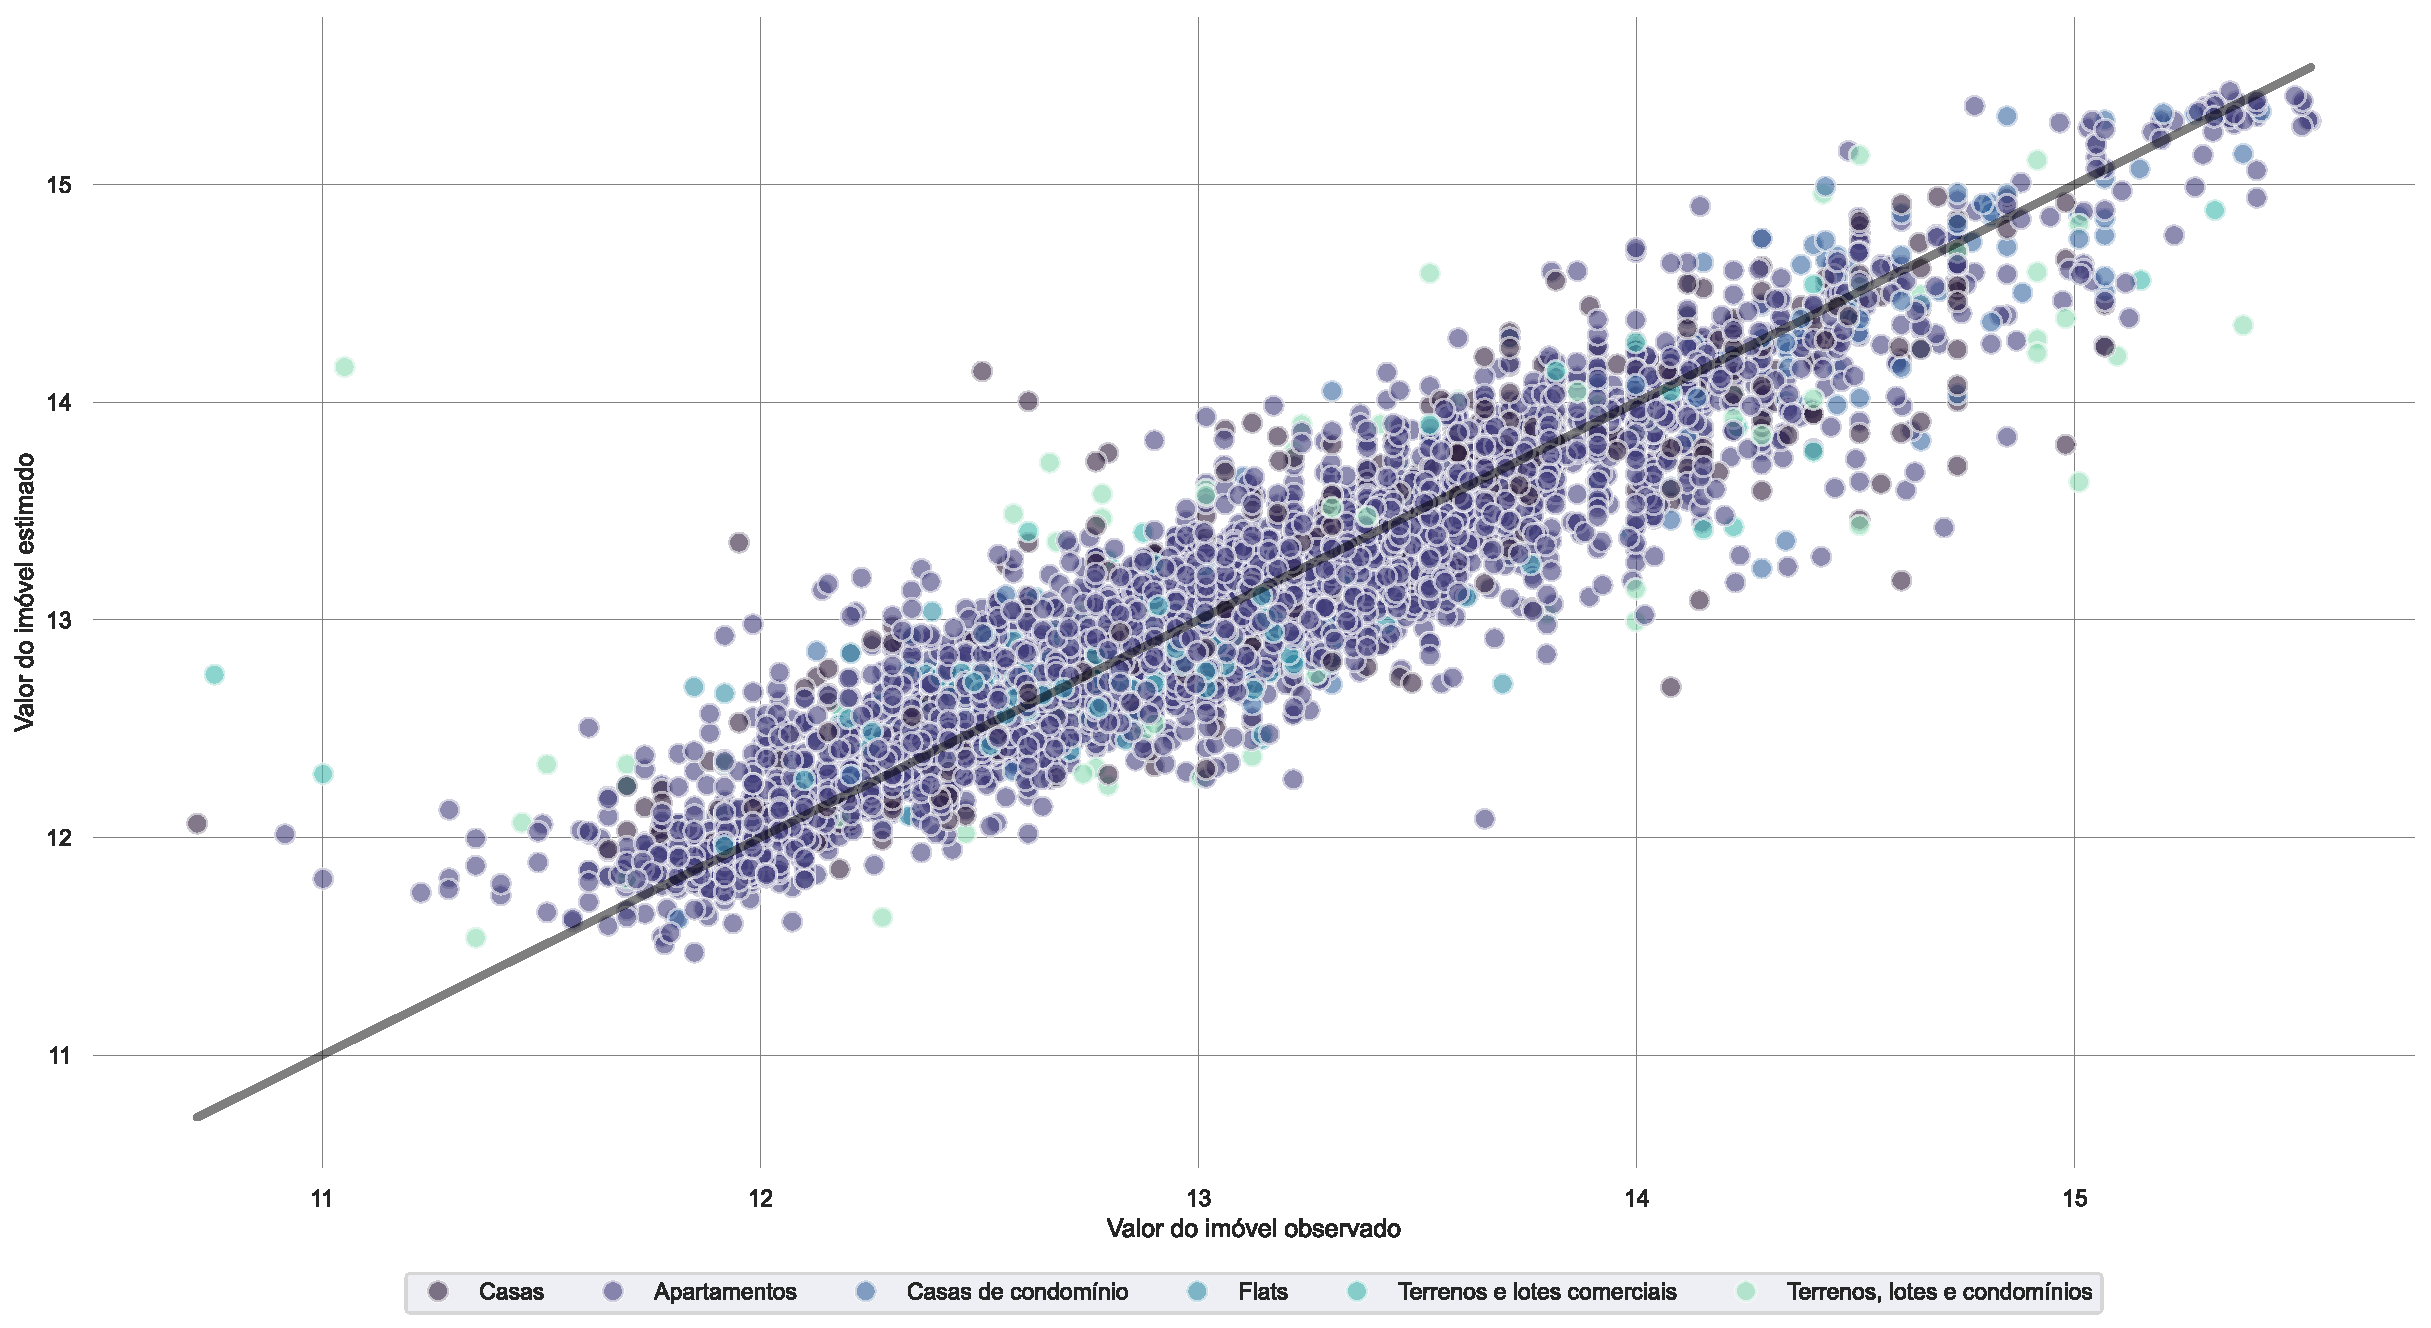
\includegraphics{TCC_files/mediabag/includes/lgbm_plot_predict.pdf}

}

\subcaption{\label{fig-preds_lgbm}}

\end{minipage}%
%
\begin{minipage}{0.50\linewidth}

\centering{

\captionsetup{labelsep=none}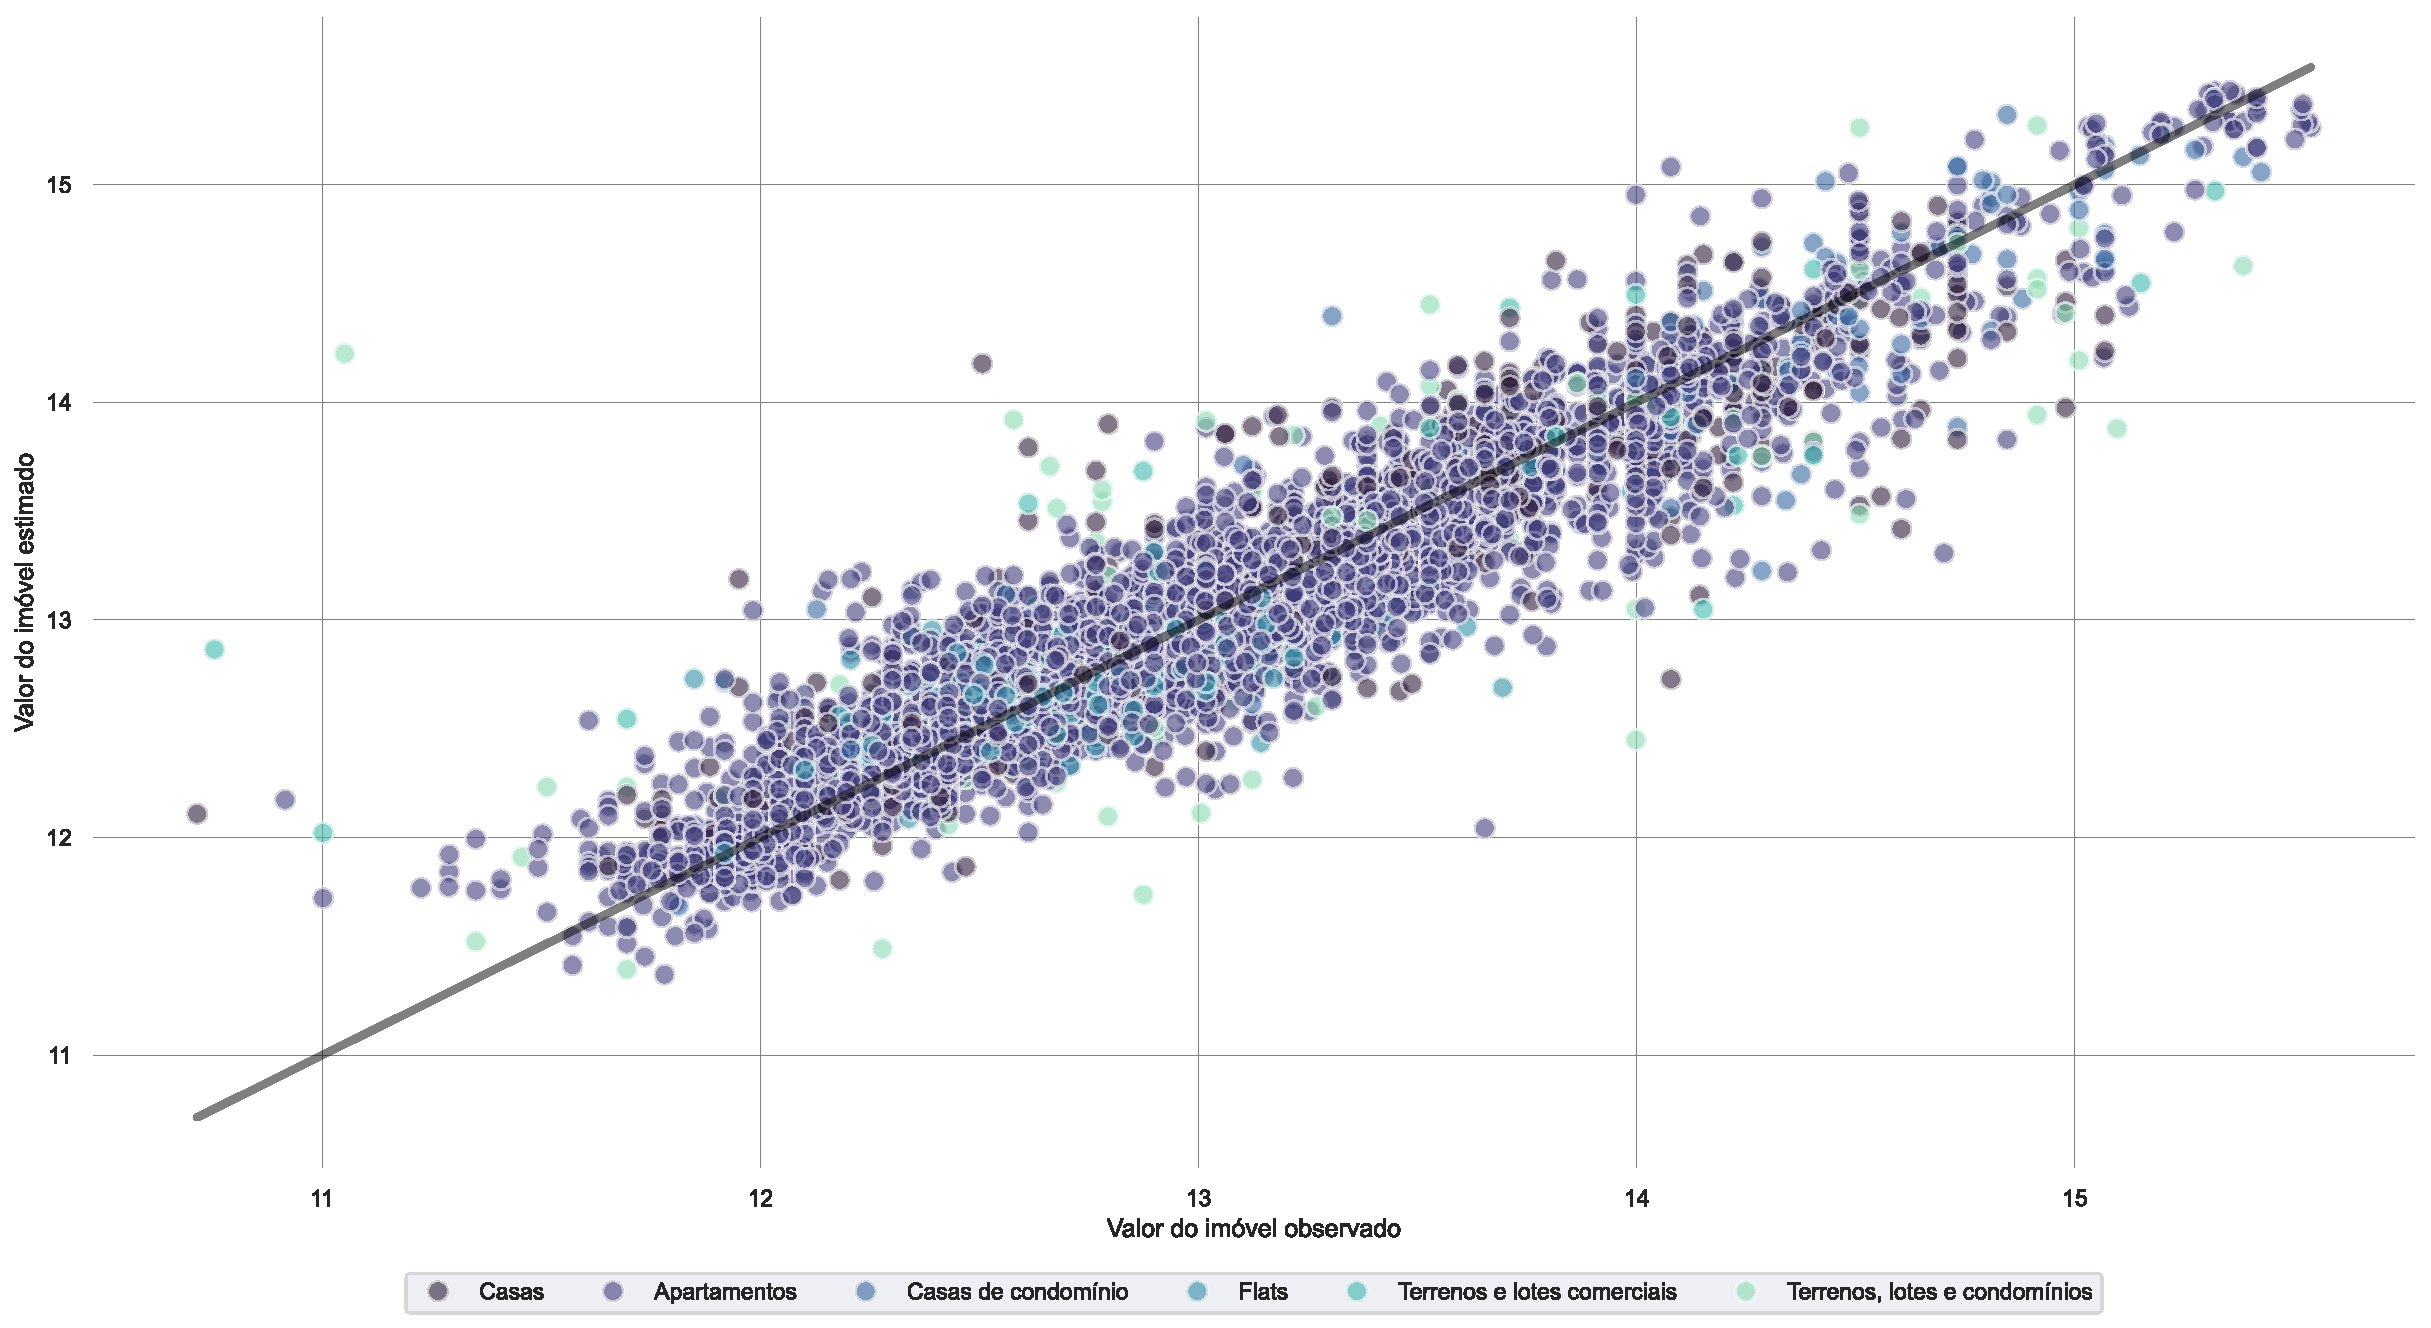
\includegraphics{TCC_files/mediabag/includes/xgb_plot_predict.pdf}

}

\subcaption{\label{fig-preds_xgb}}

\end{minipage}%

\caption{\label{fig-preds2}Valores previstos em função dos observados do
algoritmo Light Gradient Boosting e Extreme Gradient Boosting,
respectivamente.}

\end{figure}%

Assim como o LGBM, o Extreme Gradient Boosting também obteve resultados
melhores que os algoritmos de Random Forest e Gradient Boosting.
Entretanto, obteve piores em relação às estatísticas de erro de RMSE e
\(R^2\). O RMSE obtido pelo XGBoost foi de \(0,28659\) e o seu \(R^2\)
foi de \(87,03891\%\), indicando que o modelo consegue explicar
\(87,03891\%\) dos dados. No entanto, obteve um MAPE pouco menor que o
LGBM. As predições geradas pelo Extreme Gradient Boosting estão em média
\(1,357%
\) distantes de seus valores reais.

\begin{figure}

\centering{

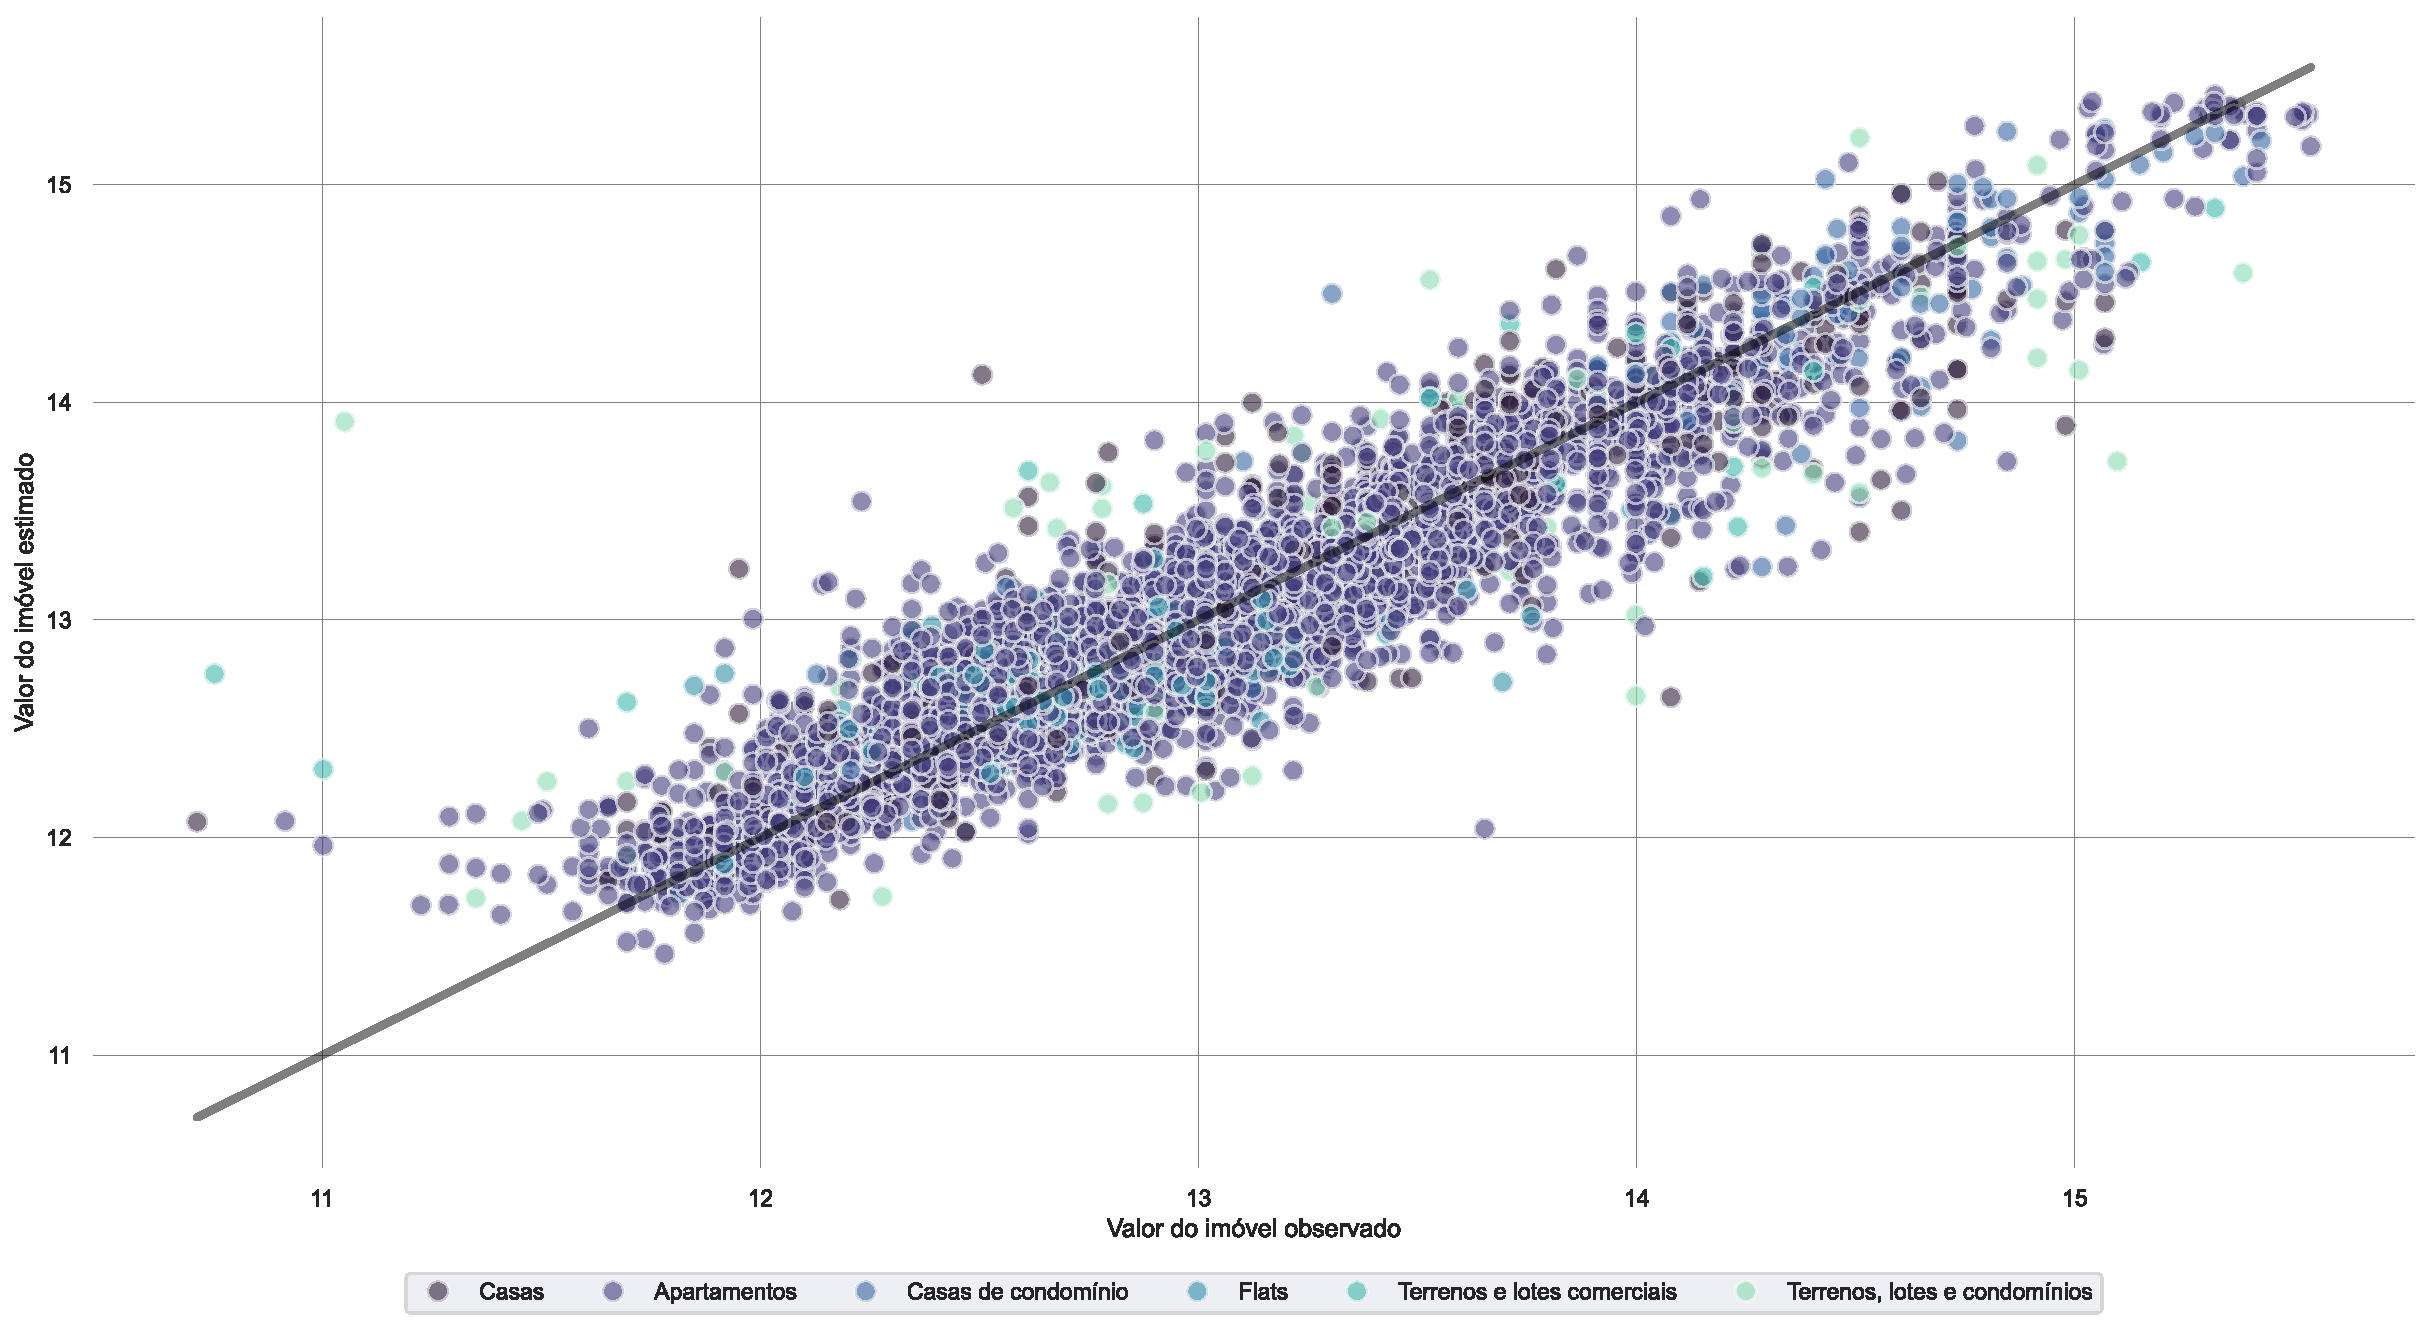
\includegraphics{TCC_files/mediabag/includes/stacking_plot_predict.pdf}

}

\caption{\label{fig-preds_stacking}Valores previstos em função dos
observados do algoritmo Stacking}

\end{figure}%

\vspace{12pt}

Utilizando os últimos modelos com seus hiperparâmetros otimizados e
utilizando o Light Gradient Boosting como estimador final, as predições
foram feitas com o Stacking. As predições geradas pelo Stacking,
analisando as métricas de erro utilizadas, foram melhores até mesmo que
o Light Gradient Boosting. O RMSE obtido para o Stacking foi de 0,28473
e o modelo consegue explicar \(87,18793\%\). A única métrica que não foi
melhor que do algoritmo LGBM foi o MAPE, que foi de \(1,357\%\), mas a
diferença é pouca.

\section{Impacto e importância das variáveis na
predição}\label{impacto-e-importuxe2ncia-das-variuxe1veis-na-prediuxe7uxe3o}

~~~O impacto e a importância das variáveis na predição de modelos são
fundamentais para entender quais fatores exercem maior influência sobre
as previsões, neste caso, para as predições de valores de imóveis. Esta
seção será dedicada à discussão do impacto das predições individuais e
da importância das variáveis utilizadas na construção do modelo. A
análise será feita com o modelo que apresentou os melhores resultados, o
algoritmo de Stacking.

\begin{figure}

\centering{

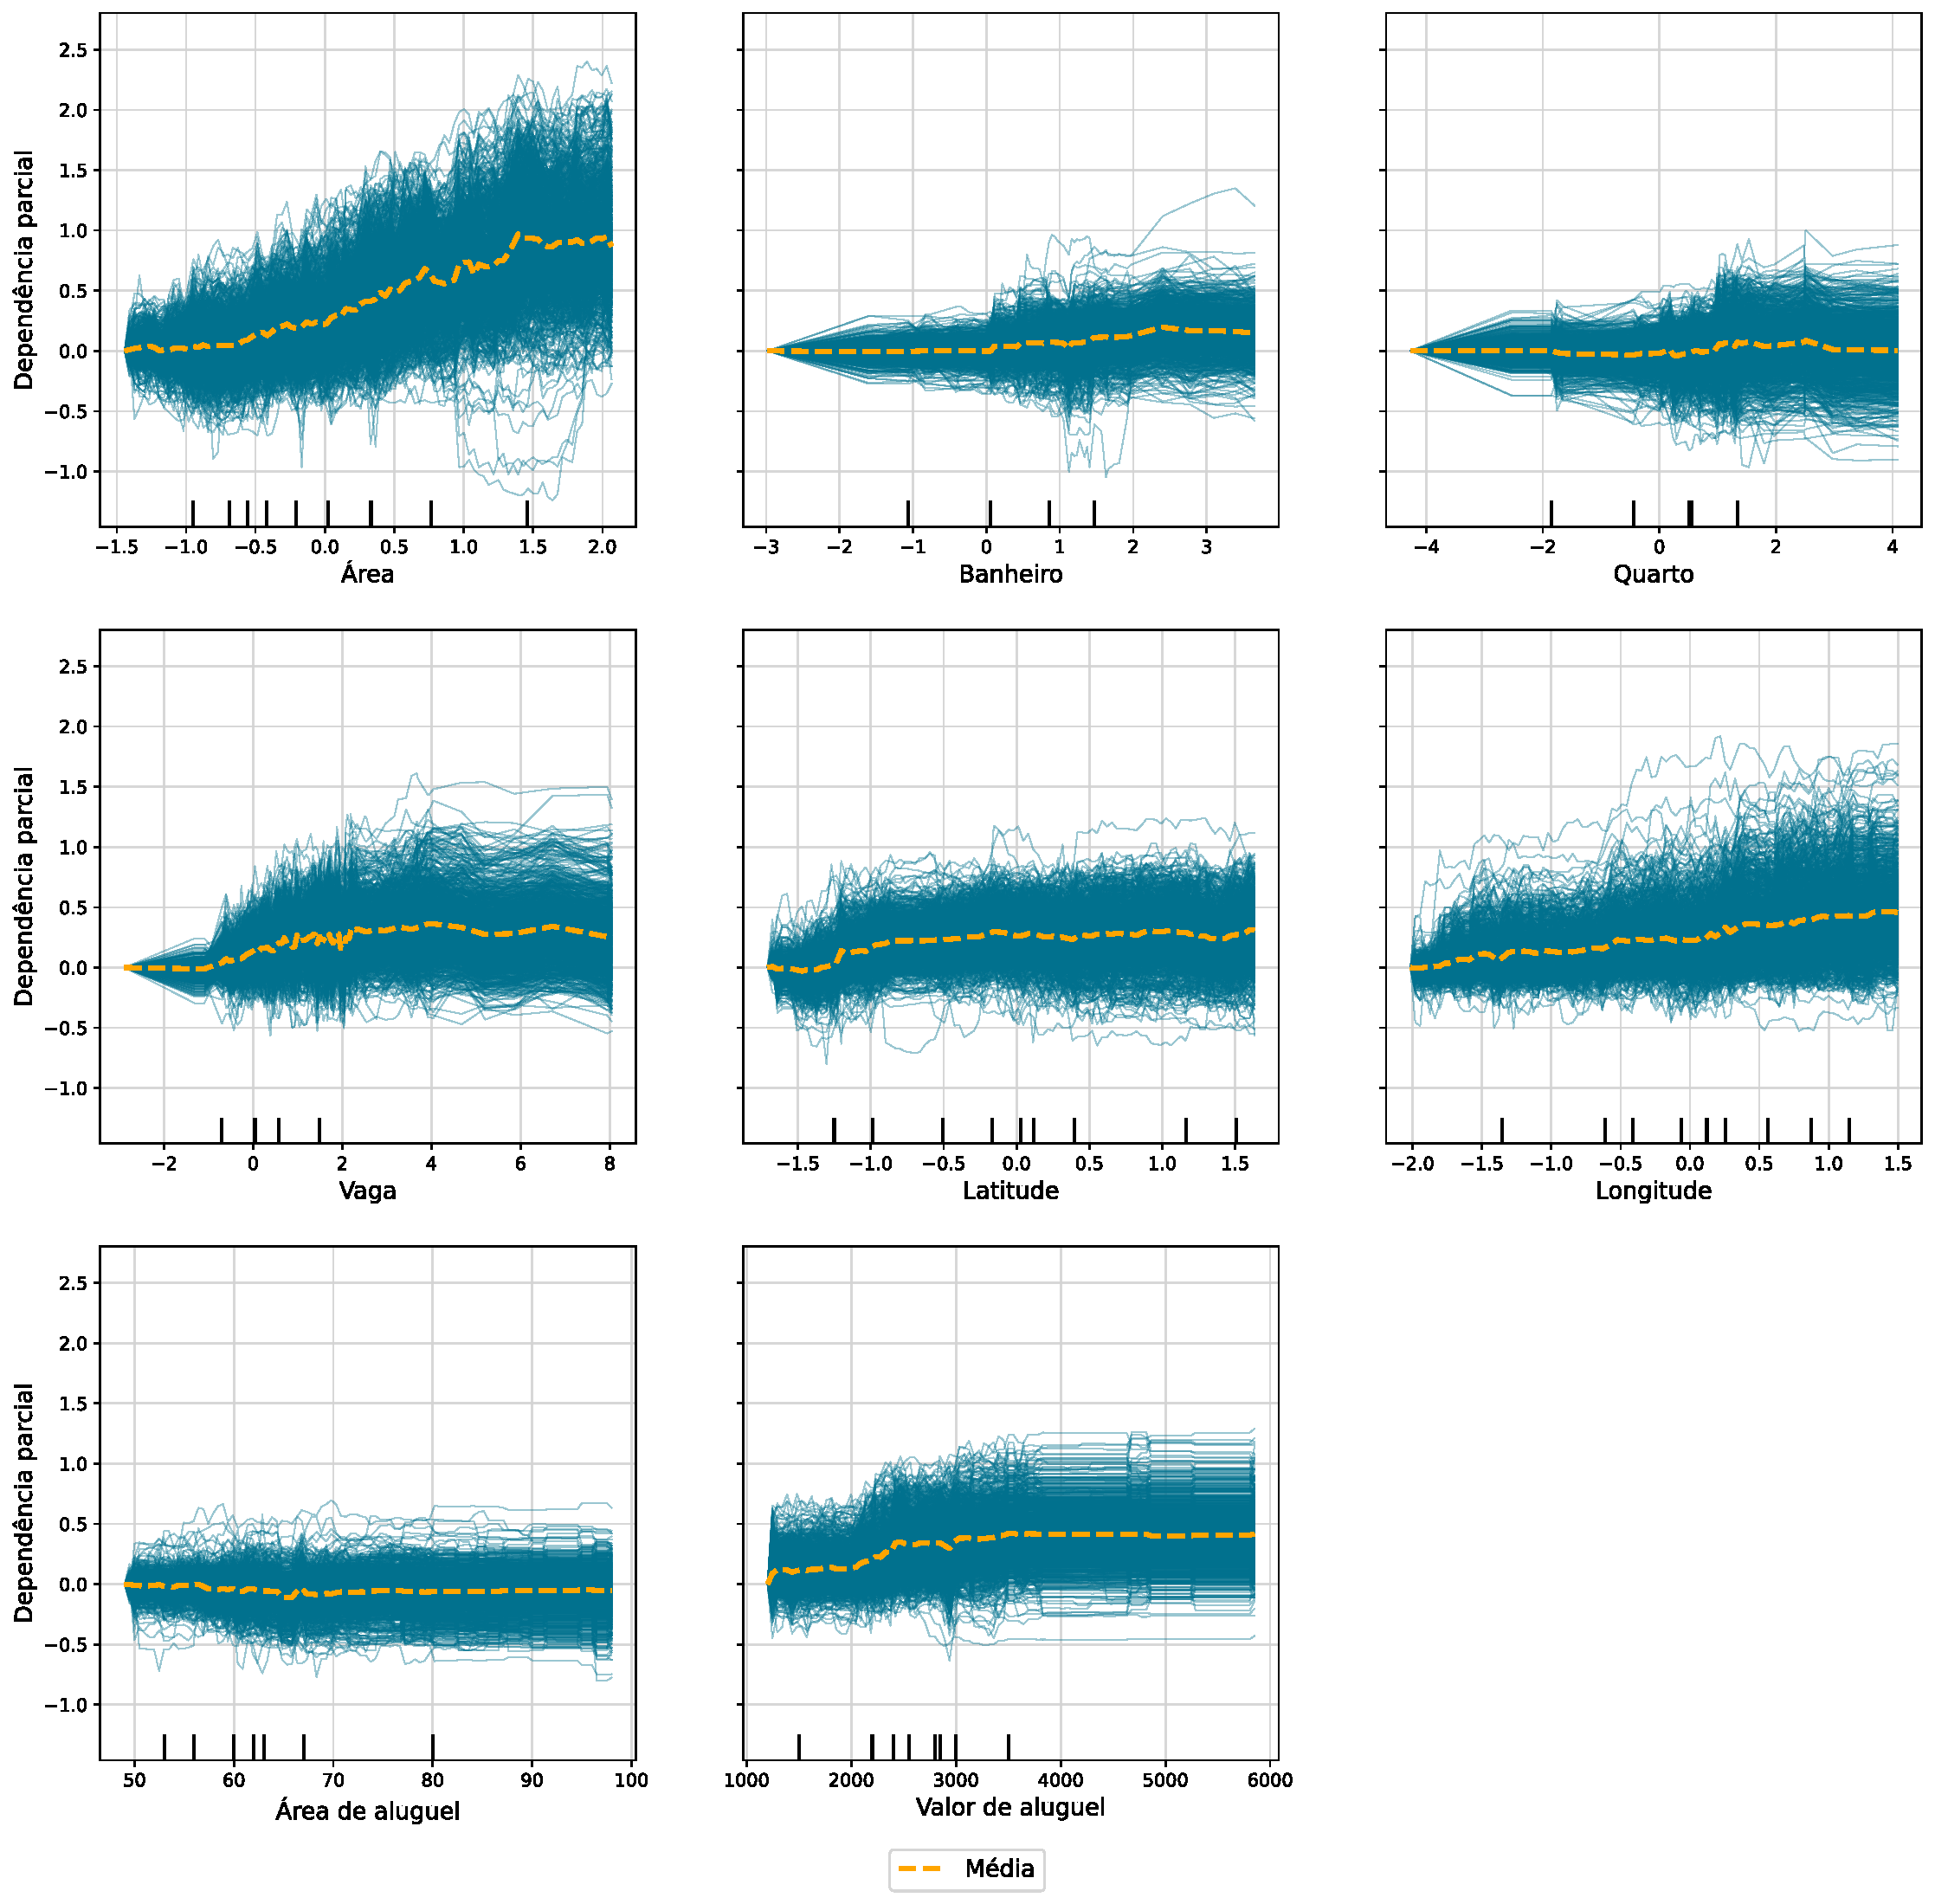
\includegraphics{TCC_files/mediabag/includes/pdp_ice.pdf}

}

\caption{\label{fig-ice_pdp}Gráfico de ICE e PDP.}

\end{figure}%

\vspace{12pt}

Para analisar a influência das variáveis na predição dos valores de
imóveis, foi utilizado o gráfico de ICE em conjunto com a linha de PDP.
Esses gráficos estão representados na Figura~\ref{fig-ice_pdp}.

\vspace{12pt}

As previsões mostram um aumento claro com o tamanho da área, com o PDP
apresentando uma tendência crescente consistente, alinhada à maioria das
curvas ICE. Para a quantidade de banheiro, a relação é majoritariamente
plana, com apenas pequenas variações. Um comportamento semelhante é
observado para a quantidade de quartos, indicando uma influência
limitada dessas variáveis no modelo. No caso do valor médio de aluguel,
o PDP revela uma tendência ascendente bem definida, e as curvas ICE
reforçam esse padrão, sugerindo que valores de aluguel mais altos estão
fortemente associados a preços de imóveis mais elevados. Já a área média
de aluguel apresenta um padrão mais uniforme, indicando uma contribuição
menos significativa para explicar os preços dos imóveis. As curvas ICE
para as coordenadas geográficas exibem um padrão mais complexo nas
previsões. No entanto, é possível identificar um aumento nos valores
previstos dos imóveis à medida que as coordenadas aumentam. Esse
comportamento sugere que os imóveis localizados mais próximos da região
litorânea de João Pessoa tendem a apresentar valores mais elevados. Por
fim, a quantidade de vagas de garagem demonstra uma relação ascendente
clara nas predições, evidenciando uma influência positiva dessa variável
no valor dos imóveis.

\begin{figure}

\begin{minipage}{0.50\linewidth}

\centering{

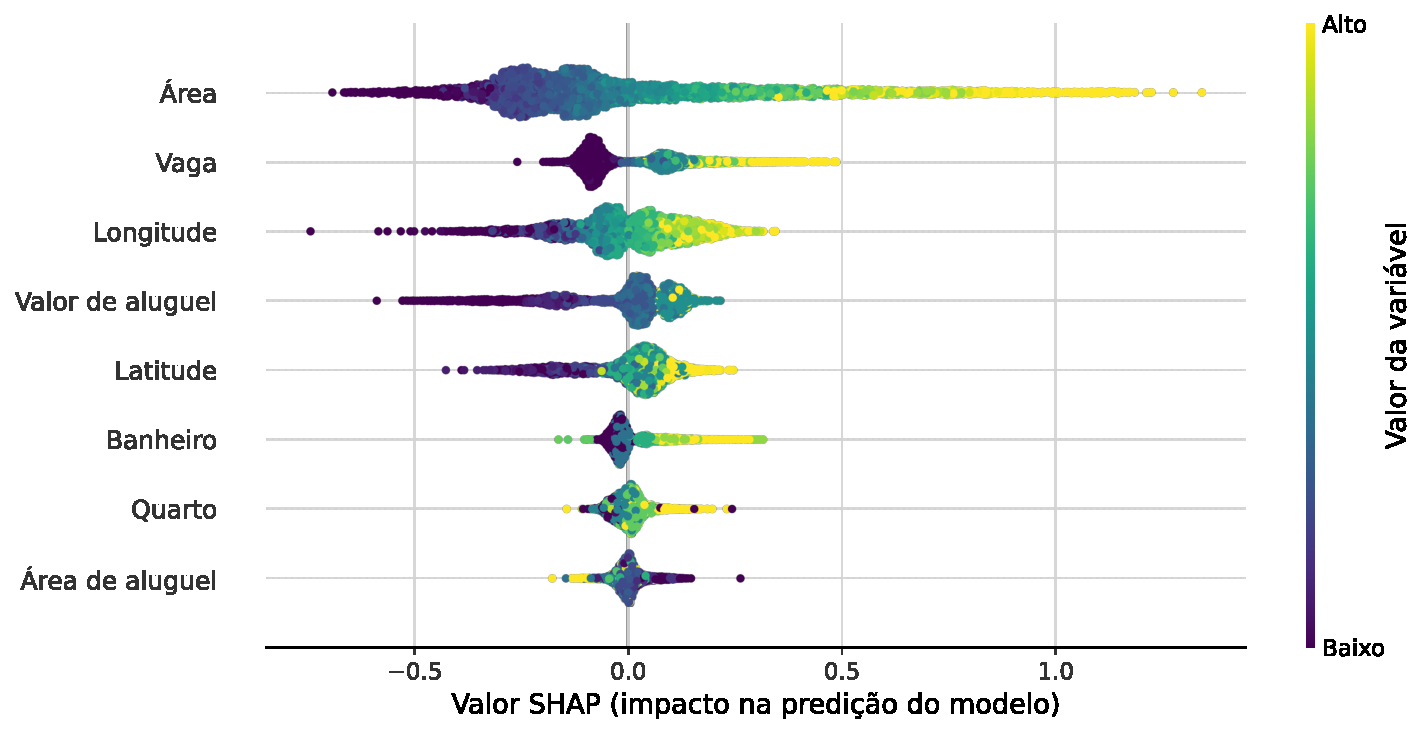
\includegraphics{TCC_files/mediabag/includes/shap_summary_plot.pdf}

}

\subcaption{\label{fig-shap_summary}Gráfico de resumo dos valores SHAP.}

\end{minipage}%
%
\begin{minipage}{0.50\linewidth}

\centering{

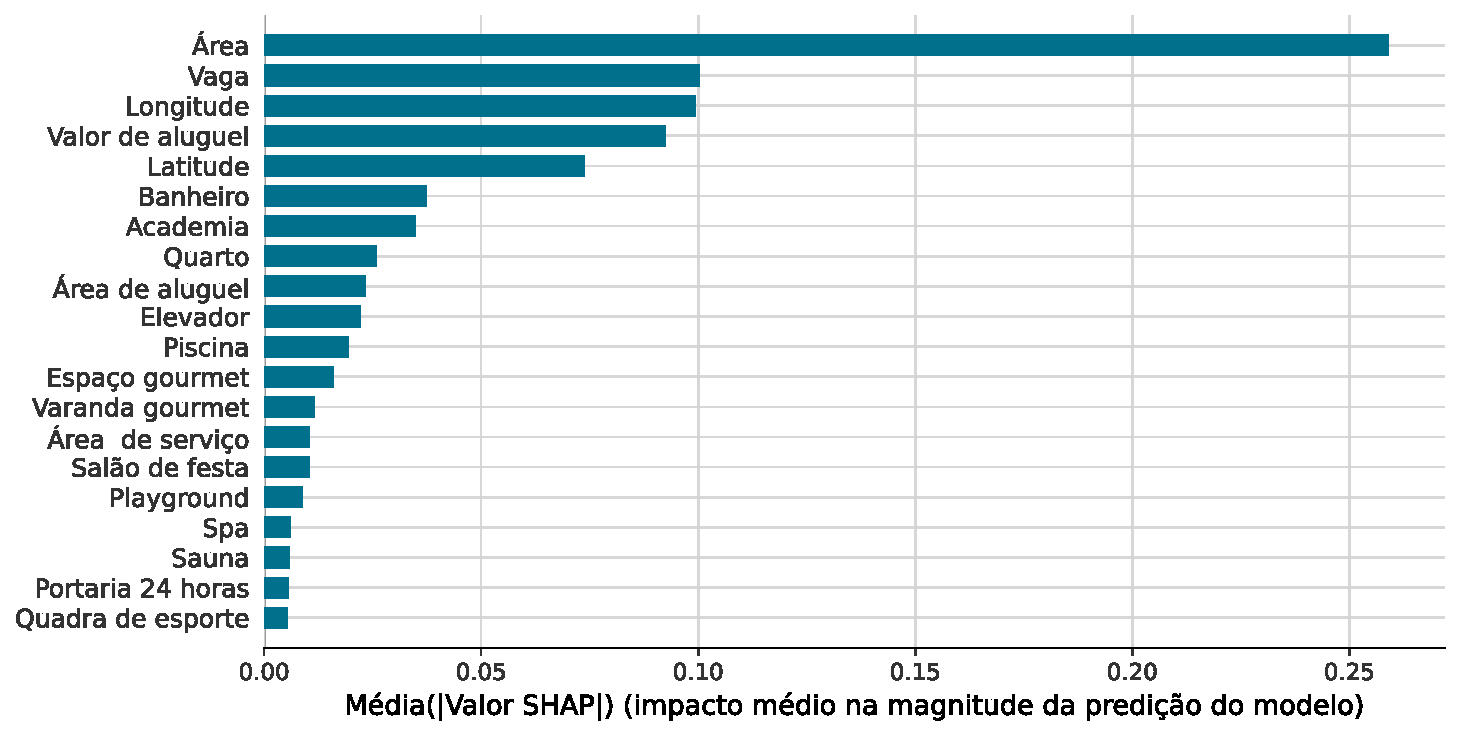
\includegraphics{TCC_files/mediabag/includes/shap_importance.pdf}

}

\subcaption{\label{fig-shap_importance}Importância das variáveis.}

\end{minipage}%

\caption{\label{fig-teste}Impacto e importância das variáveis na
predição a partir do método SHAP.}

\end{figure}%

A análise da importância das variáveis foi realizada utilizando o método
SHAP. Diferentemente da importância de variáveis gerada por algoritmos
baseados em árvores, que é calculada com base na redução da impureza ou
no ganho de informação ao longo das divisões no modelo, o SHAP é baseado
na magnitude dos valores de Shapley atribuídos a cada variável. Dessa
forma, como pode ser observado na Figura~\ref{fig-shap_importance}, a
variável com maior impacto na predição do modelo é a área, a qual
altera, em média, mais de 25 pontos percentuais na predição absoluta dos
imóveis. A quantidade de vagas de garagem, o valor médio do aluguel e a
localização geográfica também se destacam entre as variáveis mais
relevantes na predição do valor dos imóveis.

\vspace{12pt}

Com a Figura~\ref{fig-shap_summary}, observa-se um resumo da análise dos
valores Shapley. A variável área se destaca como a de maior impacto no
modelo, especialmente para valores elevados, que aumentam
significativamente as predições. As coordenadas geográficas indicam que
valores mais altos tendem a elevar a predição do valor dos imóveis,
refletindo a valorização de imóveis localizados mais próximos às regiões
litorâneas de João Pessoa. Por outro lado, a variável de área média de
aluguel apresenta um padrão menos linear, com valores baixos ainda
gerando impacto positivo nas predições, evidenciando uma relação mais
complexa com o valor dos imóveis.

\begin{figure}

\begin{minipage}{0.33\linewidth}
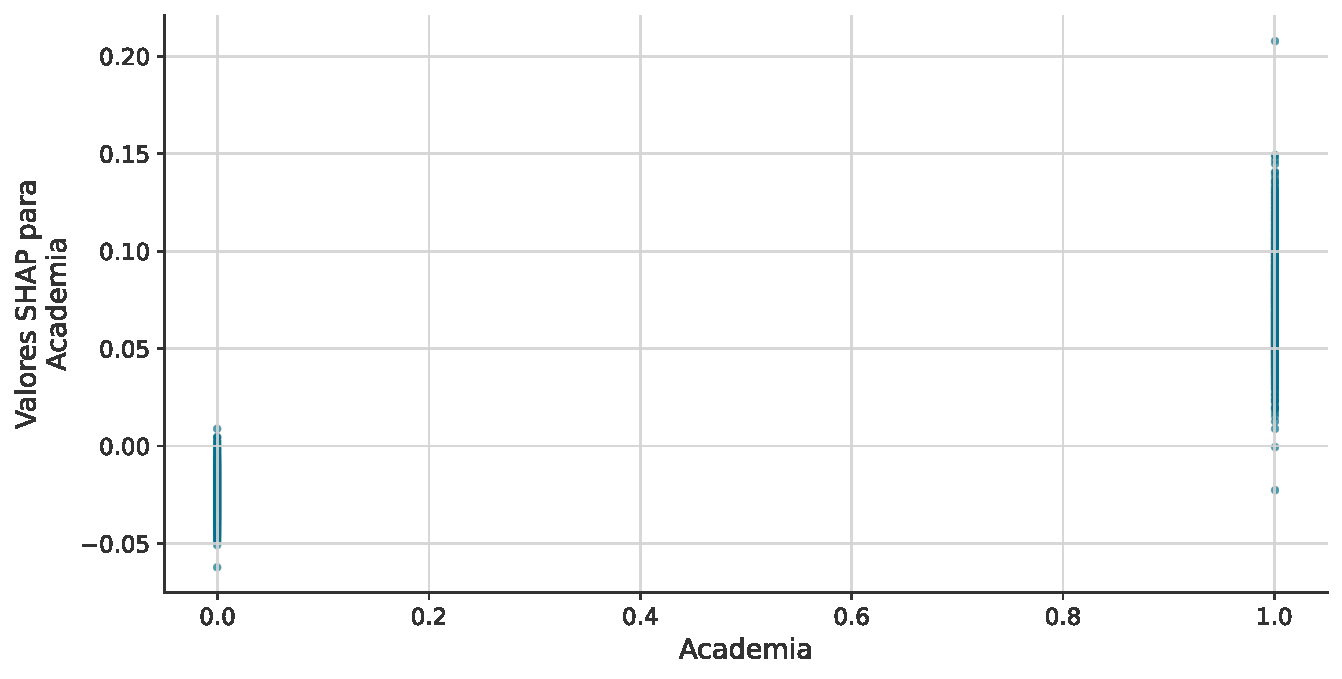
\includegraphics{TCC_files/mediabag/includes/dependence_plot_cat/dep_plot_academia.pdf}\end{minipage}%
%
\begin{minipage}{0.33\linewidth}
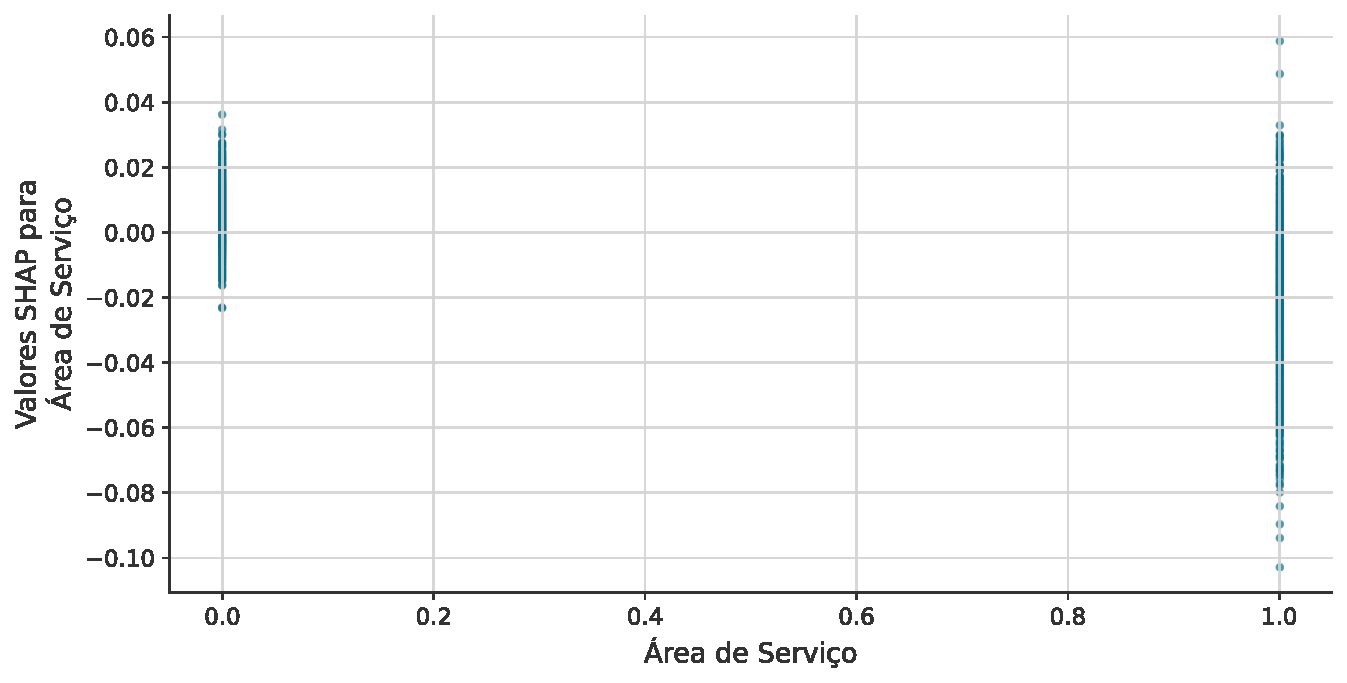
\includegraphics{TCC_files/mediabag/includes/dependence_plot_cat/dep_plot_area_servico.pdf}\end{minipage}%
%
\begin{minipage}{0.33\linewidth}
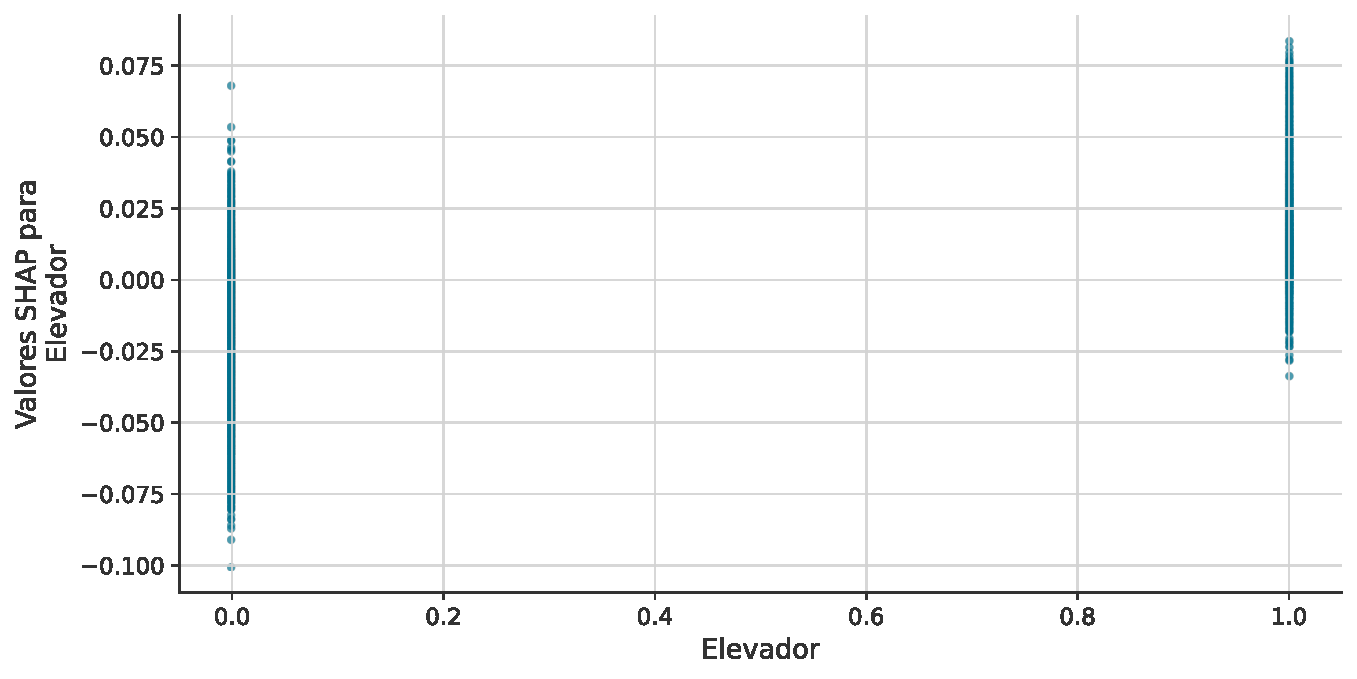
\includegraphics{TCC_files/mediabag/includes/dependence_plot_cat/dep_plot_elevador.pdf}\end{minipage}%
\newline
\begin{minipage}{0.33\linewidth}
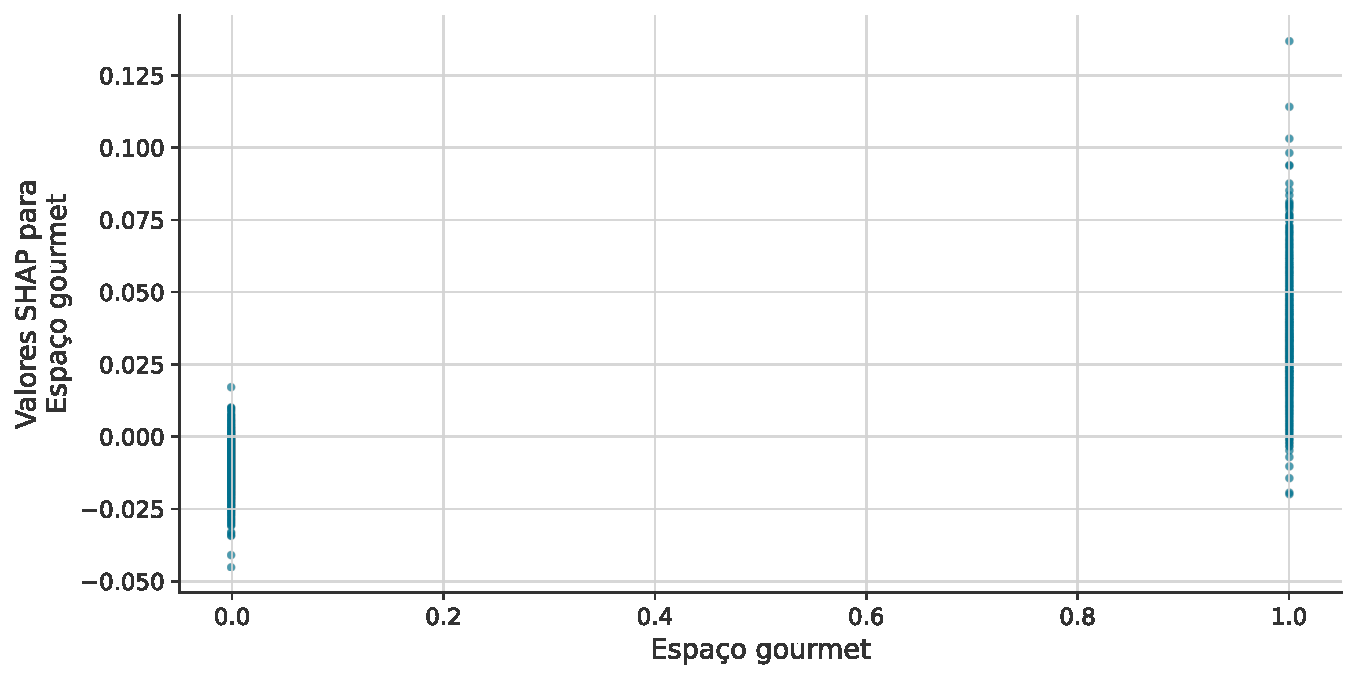
\includegraphics{TCC_files/mediabag/includes/dependence_plot_cat/dep_plot_espaco_gourmet.pdf}\end{minipage}%
%
\begin{minipage}{0.33\linewidth}
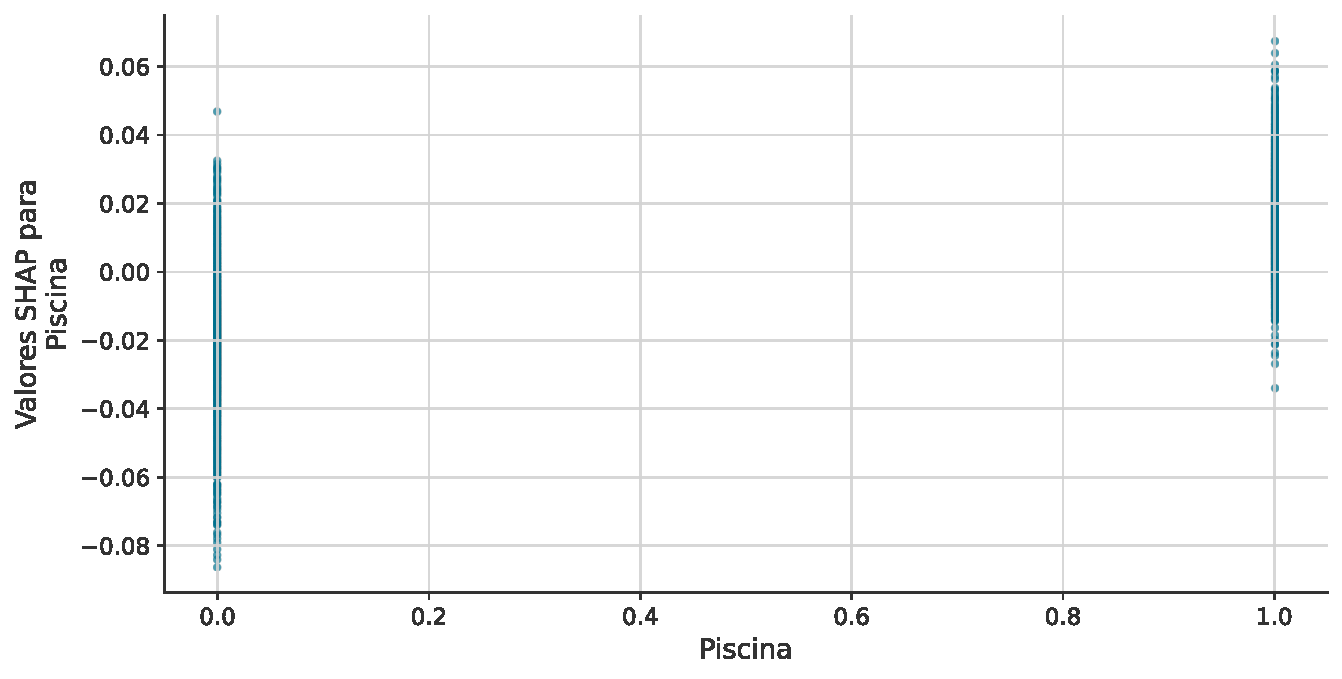
\includegraphics{TCC_files/mediabag/includes/dependence_plot_cat/dep_plot_piscina.pdf}\end{minipage}%
%
\begin{minipage}{0.33\linewidth}
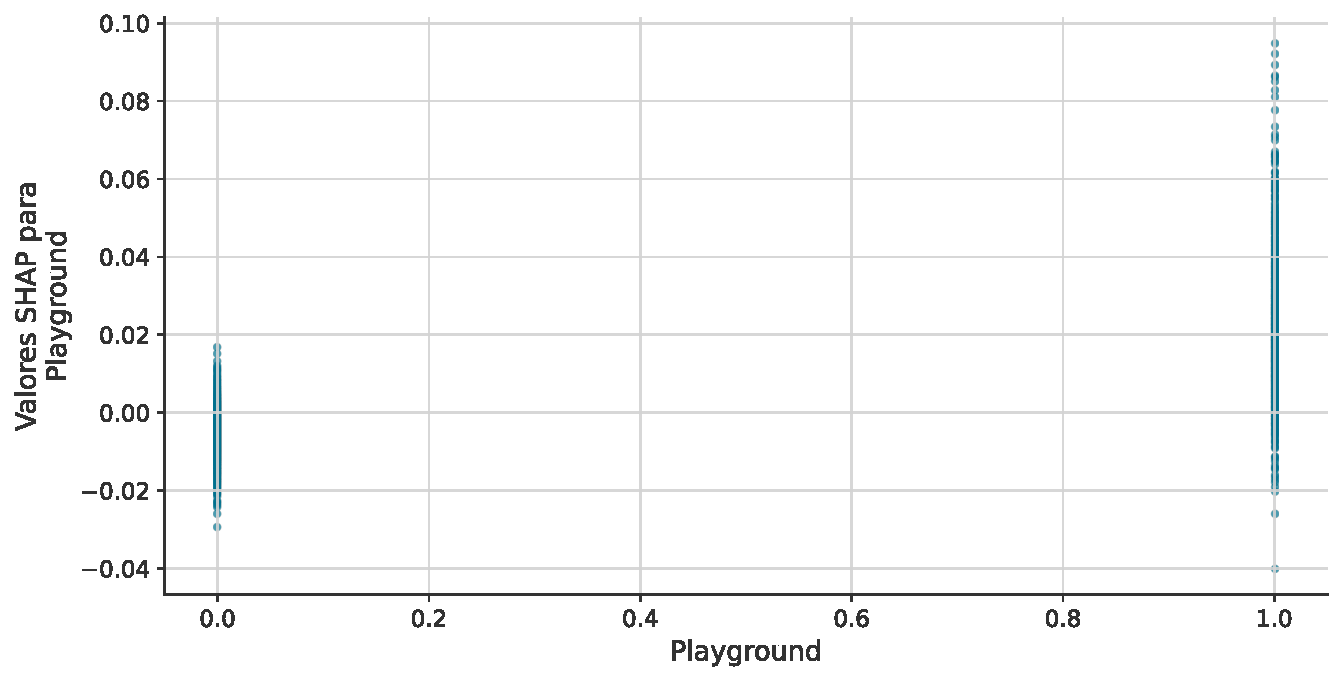
\includegraphics{TCC_files/mediabag/includes/dependence_plot_cat/dep_plot_playground.pdf}\end{minipage}%
\newline
\begin{minipage}{0.33\linewidth}
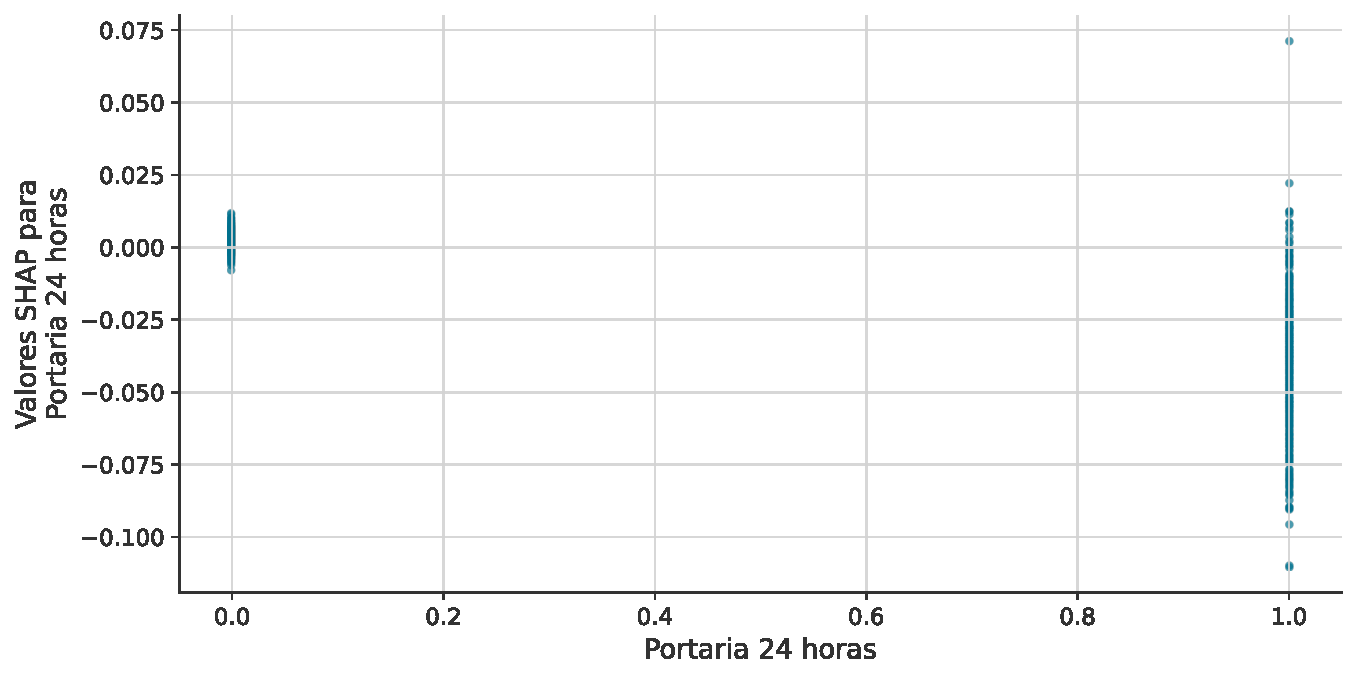
\includegraphics{TCC_files/mediabag/includes/dependence_plot_cat/dep_plot_portaria_24_horas.pdf}\end{minipage}%
%
\begin{minipage}{0.33\linewidth}
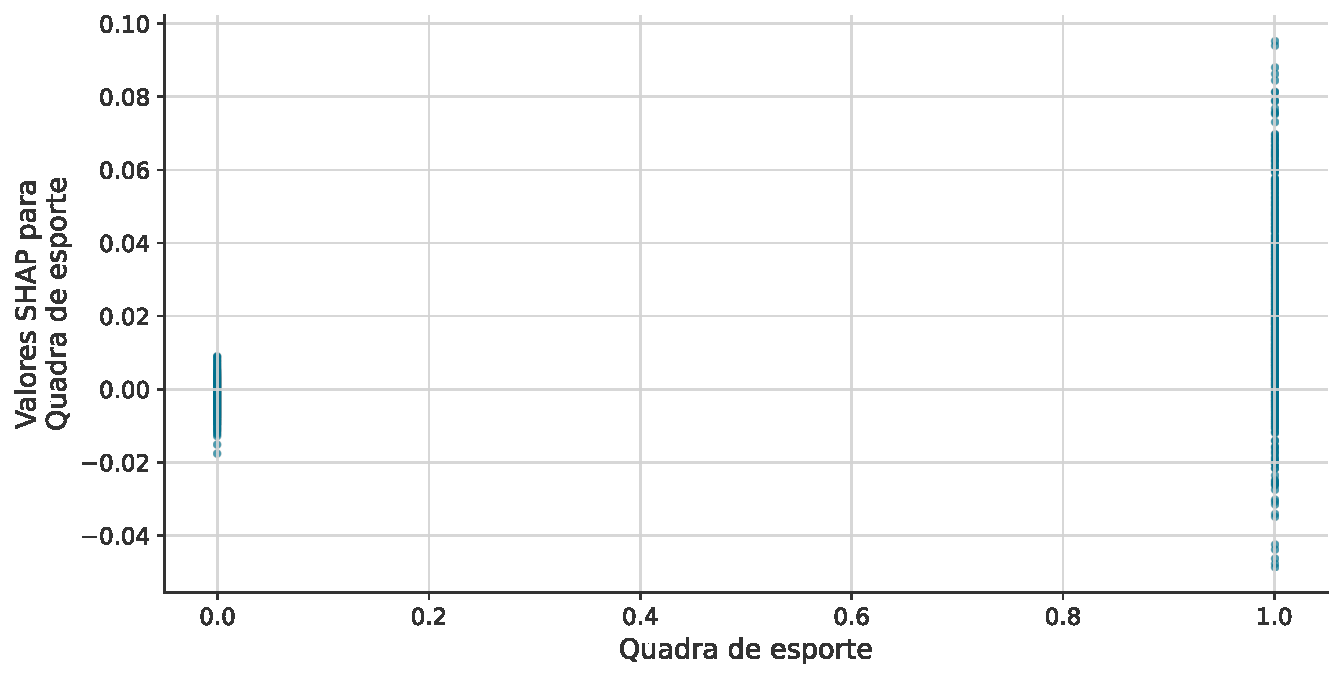
\includegraphics{TCC_files/mediabag/includes/dependence_plot_cat/dep_plot_quadra_de_esporte.pdf}\end{minipage}%
%
\begin{minipage}{0.33\linewidth}
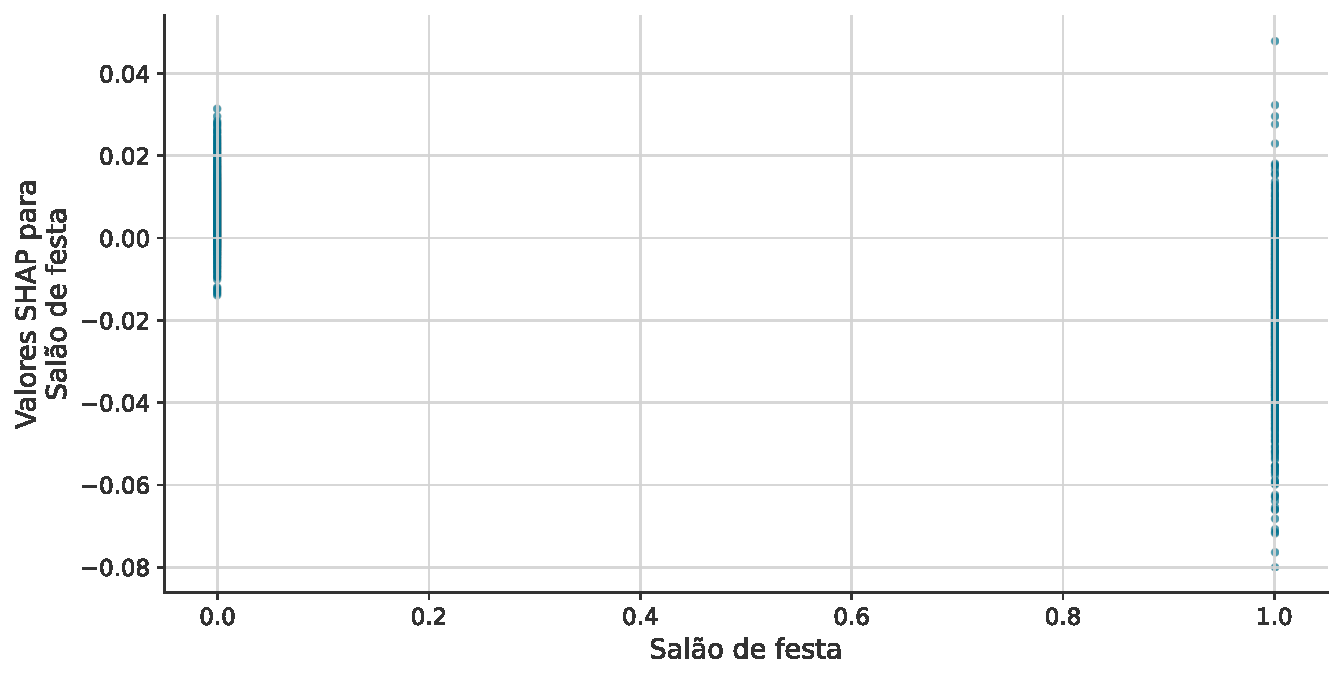
\includegraphics{TCC_files/mediabag/includes/dependence_plot_cat/dep_plot_salao_de_festa.pdf}\end{minipage}%
\newline
\begin{minipage}{0.33\linewidth}
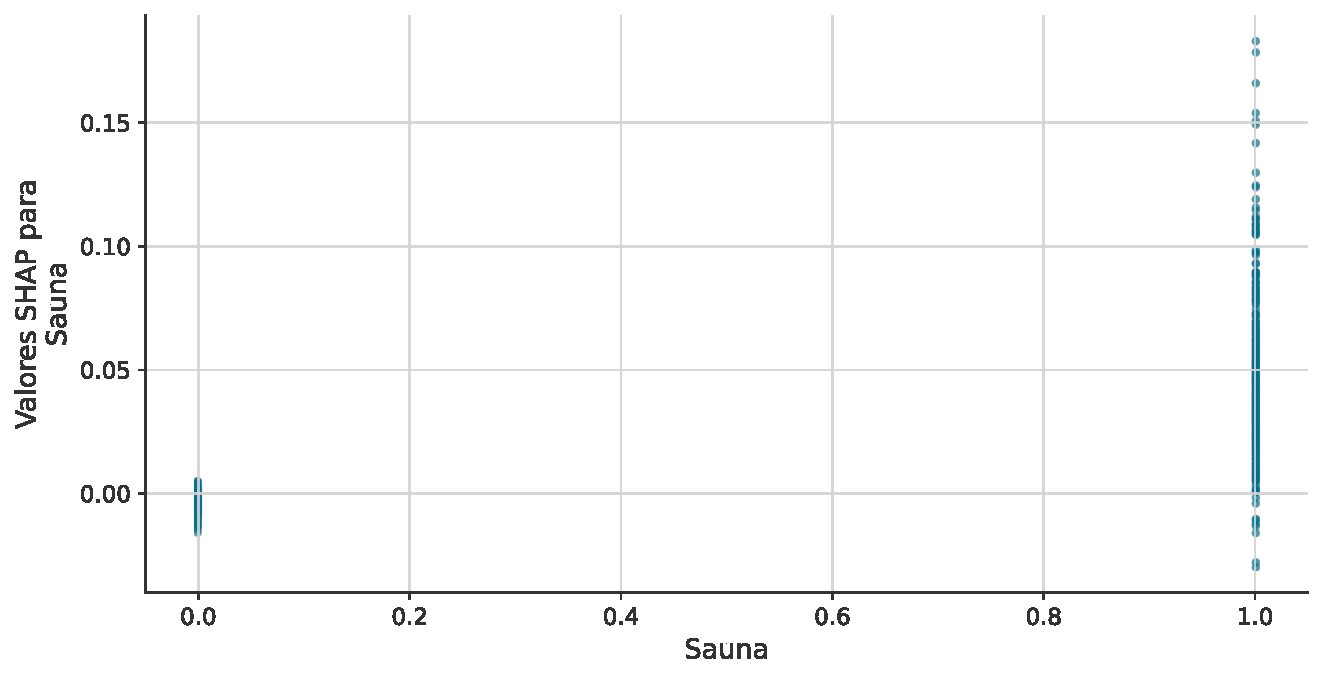
\includegraphics{TCC_files/mediabag/includes/dependence_plot_cat/dep_plot_sauna.pdf}\end{minipage}%
%
\begin{minipage}{0.33\linewidth}
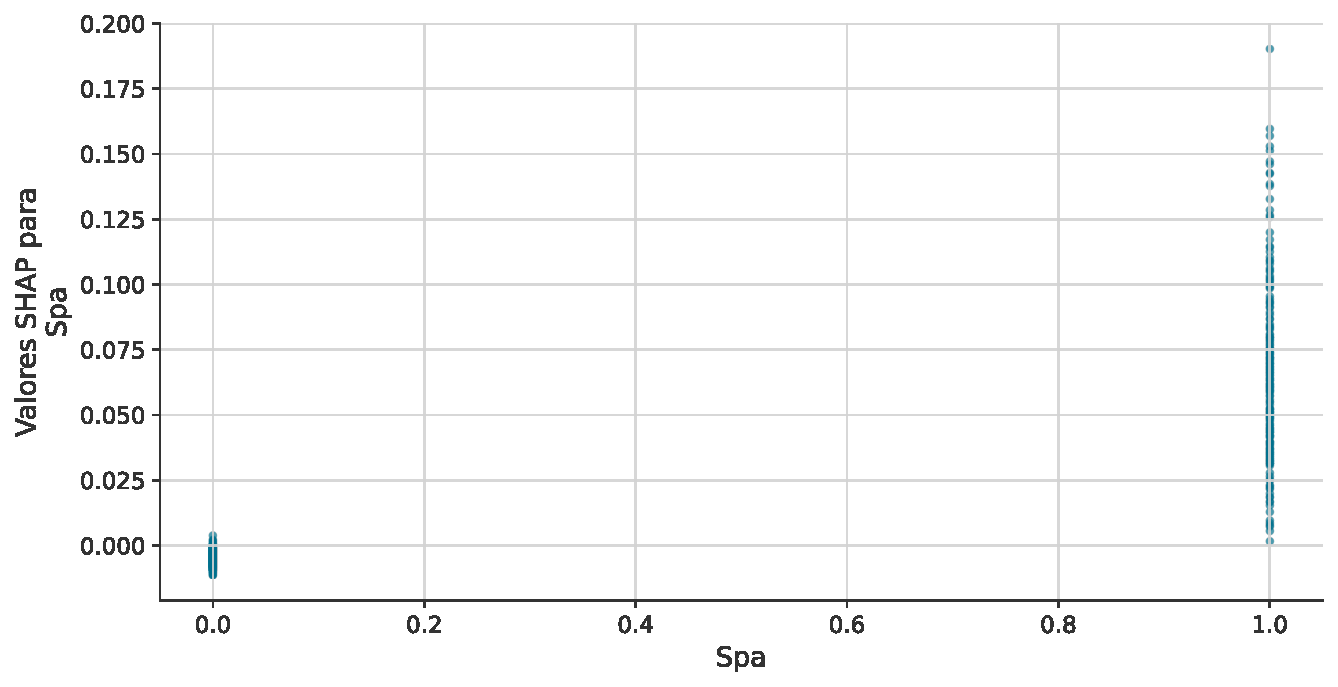
\includegraphics{TCC_files/mediabag/includes/dependence_plot_cat/dep_plot_spa.pdf}\end{minipage}%
%
\begin{minipage}{0.33\linewidth}
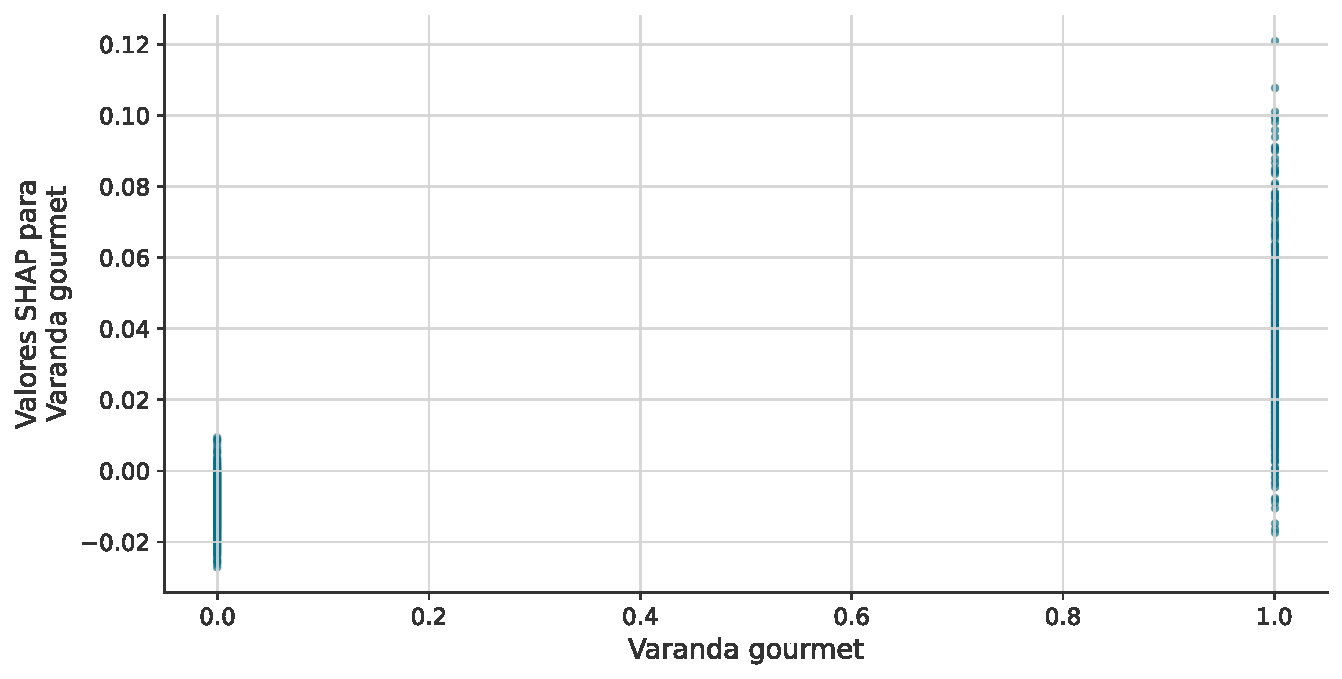
\includegraphics{TCC_files/mediabag/includes/dependence_plot_cat/dep_plot_varanda_gourmet.pdf}\end{minipage}%

\caption{\label{fig-dependence_plot}Gráfico de dependência de valores
SHAP para variáveis binárias.}

\end{figure}%

\vspace{12pt}

Para analisar as variáveis binárias, foram utilizados gráficos de
dependência para cada uma delas, os quais podem ser visualizados na
Figura~\ref{fig-dependence_plot}. Ao analisar os valores SHAP para os
imóveis com e sem academia, observa-se que essa variável tende a
aumentar a predição para imóveis que possuem academia. O mesmo padrão é
identificado para imóveis com elevador, embora aqueles sem elevador
também apresentem uma tendência de aumento na predição, o que pode ser
explicado pela influência de outras características dos imóveis. Como já
mencionado na análise da importância das variáveis, sauna e spa são
características com baixa importância. No entanto, ao observar seus
gráficos de dependência, é possível perceber que essas variáveis podem
ser úteis na avaliação de imóveis que possuem essa característica e tem
valores mais elevados. O mesmo comportamento é observado para varanda
gourmet, playground e espaço gourmet.

\chapter{Conclusão}\label{conclusuxe3o}

\chapter*{\texorpdfstring{\centering Referências}{Referências}}\label{referuxeancias}

\markboth{Referências}{Referências}

\phantomsection\label{refs}
\begin{CSLReferences}{0}{1}
\bibitem[\citeproctext]{ref-abecip_credito2007}
ABECIP. \textbf{O Crédito Imobiliário no Brasil: Caracterização e
Desafios}. {[}S.l.{]}: Associação Brasileira das Entidades de Crédito
Imobiliário e Poupança, 2007b.

\bibitem[\citeproctext]{ref-revolucao_credito_imobiliario}
\_\_\_\_\_\_. \textbf{A Revolução do Crédito Imobiliário: 44 Anos
(1967--2011)}. {[}S.l.{]}: Associação Brasileira das Entidades de
Crédito Imobiliário e Poupança, 2007a.

\bibitem[\citeproctext]{ref-abecip_monografia}
\_\_\_\_\_\_. \textbf{IV Prêmio ABECIP de Monografia em Crédito
Imobiliário e Poupança}. {[}S.l.{]}: Associação Brasileira das Entidades
de Crédito Imobiliário e Poupança, 2015.

\bibitem[\citeproctext]{ref-optuna_2019}
AKIBA, T. \emph{et al.} Optuna: A Next-generation Hyperparameter
Optimization Framework. {[}S.l.{]}: {[}s.n.{]}, 2019.

\bibitem[\citeproctext]{ref-quarto}
ALLAIRE, J.; DERVIEUX, C.
\textbf{\href{https://CRAN.R-project.org/package=quarto}{quarto: R
Interface to 'Quarto' Markdown Publishing System}}. {[}S.l.{]}:
{[}s.n.{]}, 2024.

\bibitem[\citeproctext]{ref-assumpccao2011credito}
ASSUMPÇÃO FILHO, C. A. B. O cr{é}dito imobili{á}rio no Brasil. 2011.

\bibitem[\citeproctext]{ref-bergstra2011algorithms}
BERGSTRA, J. \emph{et al.} Algorithms for hyper-parameter optimization.
\textbf{Advances in neural information processing systems}, 2011. v. 24.

\bibitem[\citeproctext]{ref-bergstra2013making}
\_\_\_\_\_\_; YAMINS, D.; COX, D. Making a science of model search:
Hyperparameter optimization in hundreds of dimensions for vision
architectures. {[}S.l.{]}: PMLR, 2013. p. 115--123.

\bibitem[\citeproctext]{ref-bischl2023hyperparameter}
BISCHL, B. \emph{et al.} Hyperparameter optimization: Foundations,
algorithms, best practices, and open challenges. \textbf{Wiley
Interdisciplinary Reviews: Data Mining and Knowledge Discovery}, 2023.
v. 13, n. 2, p. e1484.

\bibitem[\citeproctext]{ref-breiman1996bagging}
BREIMAN, L. Bagging predictors. \textbf{Machine learning}, 1996. v. 24,
p. 123--140.

\bibitem[\citeproctext]{ref-geocoder}
CAMBON, J. \emph{et al.} tidygeocoder: An R package for geocoding.
\textbf{Journal of Open Source Software}, 2021. v. 6, n. 65, p. 3544.
Disponível em:
\textless{}\url{https://doi.org/10.21105/joss.03544}\textgreater.

\bibitem[\citeproctext]{ref-campos2014precificaccao}
CAMPOS, S. F. Precifica{ç}{ã}o de im{ó}veis e seus elementos agregadores
de valor sob a vis{ã}o do consumidor: uma an{á}lise do mercado
imobili{á}rio de Jo{ã}o Pessoa-PB. 2014.

\bibitem[\citeproctext]{ref-chen2016xgboost}
CHEN, T.; GUESTRIN, C. Xgboost: A scalable tree boosting system.
{[}S.l.{]}: {[}s.n.{]}, 2016. p. 785--794.

\bibitem[\citeproctext]{ref-evolucao_abecip}
COSTA FARIAS, B. M. Da. A evolu{ç}{ã}o do mercado imobili{á}rio
brasileiro e o conceito de Home Equity. 2010.

\bibitem[\citeproctext]{ref-cowen2022hebo}
COWEN-RIVERS, A. I. \emph{et al.} Hebo: Pushing the limits of
sample-efficient hyper-parameter optimisation. \textbf{Journal of
Artificial Intelligence Research}, 2022. v. 74, p. 1269--1349.

\bibitem[\citeproctext]{ref-fipe_metodologia}
FIPE -- FUNDAÇÃO INSTITUTO DE PESQUISAS ECONÔMICAS. \textbf{Índice
FipeZap de Preços de Imóveis Anunciados: Notas Metodológicas}. São
Paulo: Fipe, 2024.

\bibitem[\citeproctext]{ref-friedman2002stochastic}
FRIEDMAN, J. H. Stochastic gradient boosting. \textbf{Computational
statistics \& data analysis}, 2002. v. 38, n. 4, p. 367--378.

\bibitem[\citeproctext]{ref-garnett2023bayesian}
GARNETT, R. \textbf{Bayesian optimization}. {[}S.l.{]}: Cambridge
University Press, 2023.

\bibitem[\citeproctext]{ref-goldstein2015peeking}
GOLDSTEIN, A. \emph{et al.} Peeking inside the black box: Visualizing
statistical learning with plots of individual conditional expectation.
\textbf{journal of Computational and Graphical Statistics}, 2015. v. 24,
n. 1, p. 44--65.

\bibitem[\citeproctext]{ref-hastie2009elements}
HASTIE, T. \emph{et al.} \textbf{The elements of statistical learning:
data mining, inference, and prediction}. {[}S.l.{]}: Springer, 2009. V.
2.

\bibitem[\citeproctext]{ref-Hunter:2007}
HUNTER, J. D. \href{https://doi.org/10.1109/MCSE.2007.55}{Matplotlib: A
2D graphics environment}. \textbf{Computing in Science \& Engineering},
2007. v. 9, n. 3, p. 90--95.

\bibitem[\citeproctext]{ref-james2013introduction}
JAMES, G. \emph{et al.} \textbf{An introduction to statistical
learning}. {[}S.l.{]}: Springer, 2013. V. 112.

\bibitem[\citeproctext]{ref-kouzis2016learning}
KOUZIS-LOUKAS, D. \textbf{Learning Scrapy}. {[}S.l.{]}: Packt Publishing
Ltd, 2016.

\bibitem[\citeproctext]{ref-NIPS2017_7062}
LUNDBERG, S. M.; LEE, S.-I.
\href{http://papers.nips.cc/paper/7062-a-unified-approach-to-interpreting-model-predictions.pdf}{A
Unified Approach to Interpreting Model Predictions}. \emph{Em}: GUYON,
I. \emph{et al.} (Org.). \textbf{Advances in Neural Information
Processing Systems 30}. {[}S.l.{]}: Curran Associates, Inc., 2017, p.
4765--4774.

\bibitem[\citeproctext]{ref-mckinney-proc-scipy-2010}
MCKINNEY, Wes.
\href{https://doi.org/\%2010.25080/Majora-92bf1922-00a\%20}{{D}ata
{S}tructures for {S}tatistical {C}omputing in {P}ython}. (Stéfan van der
Walt \& Jarrod Millman, Org.). {[}S.l.{]}: {[}s.n.{]}, 2010. p. 56--61.

\bibitem[\citeproctext]{ref-molnar2020interpretable}
MOLNAR, C. \textbf{Interpretable machine learning}. {[}S.l.{]}: Lulu.
com, 2020.

\bibitem[\citeproctext]{ref-scikit-learn}
PEDREGOSA, F. \emph{et al.} Scikit-learn: Machine Learning in {P}ython.
\textbf{Journal of Machine Learning Research}, 2011. v. 12, p.
2825--2830.

\bibitem[\citeproctext]{ref-r_language}
R CORE TEAM. \textbf{\href{https://www.R-project.org/}{R: A Language and
Environment for Statistical Computing}}. Vienna, Austria: R Foundation
for Statistical Computing, 2024.

\bibitem[\citeproctext]{ref-ribeiro2016should}
RIBEIRO, M. T.; SINGH, S.; GUESTRIN, C. " Why should i trust you?"
Explaining the predictions of any classifier. {[}S.l.{]}: {[}s.n.{]},
2016. p. 1135--1144.

\bibitem[\citeproctext]{ref-richardson2007beautiful}
RICHARDSON, L. Beautiful soup documentation. \textbf{April}, 2007.

\bibitem[\citeproctext]{ref-shapley1953value}
SHAPLEY, L. S. A value for n-person games. \textbf{Contribution to the
Theory of Games}, 1953. v. 2.

\bibitem[\citeproctext]{ref-snoek2012practical}
SNOEK, J.; LAROCHELLE, H.; ADAMS, R. P. Practical bayesian optimization
of machine learning algorithms. \textbf{Advances in neural information
processing systems}, 2012. v. 25.

\bibitem[\citeproctext]{ref-vstrumbelj2014explaining}
ŠTRUMBELJ, E.; KONONENKO, I. Explaining prediction models and individual
predictions with feature contributions. \textbf{Knowledge and
information systems}, 2014. v. 41, p. 647--665.

\bibitem[\citeproctext]{ref-reback2020pandas}
TEAM, T. Pandas Development. \textbf{pandas-dev/pandas: Pandas}. Zenodo.
Disponível em:
\textless{}\url{https://doi.org/10.5281/zenodo.3509134}\textgreater.

\bibitem[\citeproctext]{ref-selenium}
THORPE, A.
\textbf{\href{https://CRAN.R-project.org/package=selenium}{selenium:
Low-Level Browser Automation Interface}}. {[}S.l.{]}: {[}s.n.{]}, 2024.

\bibitem[\citeproctext]{ref-van1995python}
VAN ROSSUM, G.; DRAKE JR, F. L. \textbf{Python reference manual}.
{[}S.l.{]}: Centrum voor Wiskunde en Informatica Amsterdam, 1995.

\bibitem[\citeproctext]{ref-wagner1980urbanization}
WAGNER, F. E.; WARD, J. O. Urbanization and Migration in Brazil.
\textbf{The American Journal of Economics and Sociology}, 1980. v. 39,
n. 3, p. 249--259.

\bibitem[\citeproctext]{ref-Waskom2021}
WASKOM, M. L. seaborn: statistical data visualization. \textbf{Journal
of Open Source Software}, 2021. v. 6, n. 60, p. 3021. Disponível em:
\textless{}\url{https://doi.org/10.21105/joss.03021}\textgreater.

\bibitem[\citeproctext]{ref-httr}
WICKHAM, H. \textbf{\href{https://CRAN.R-project.org/package=httr}{httr:
Tools for Working with URLs and HTTP}}. {[}S.l.{]}: {[}s.n.{]}, 2023.

\bibitem[\citeproctext]{ref-rvest}
\_\_\_\_\_\_. \textbf{\href{https://rvest.tidyverse.org/}{rvest: Easily
Harvest (Scrape) Web Pages}}. {[}S.l.{]}: {[}s.n.{]}, 2024.

\bibitem[\citeproctext]{ref-xml2}
\_\_\_\_\_\_; HESTER, J.; OOMS, J.
\textbf{\href{https://xml2.r-lib.org/}{xml2: Parse XML}}. {[}S.l.{]}:
{[}s.n.{]}, 2023.

\bibitem[\citeproctext]{ref-yang2020hyperparameter}
YANG, L.; SHAMI, A. On hyperparameter optimization of machine learning
algorithms: Theory and practice. \textbf{Neurocomputing}, 2020. v. 415,
p. 295--316.

\end{CSLReferences}



\end{document}
